%% uctest.tex 11/3/94
%% Copyright (C) 1988-2004 Daniel Gildea, BBF, Ethan Munson.
%
% This work may be distributed and/or modified under the
% conditions of the LaTeX Project Public License, either version 1.3
% of this license or (at your option) any later version.
% The latest version of this license is in
%   http://www.latex-project.org/lppl.txt
% and version 1.3 or later is part of all distributions of LaTeX
% version 2003/12/01 or later.
%
% This work has the LPPL maintenance status "maintained".
% 
% The Current Maintainer of this work is Daniel Gildea.
\documentclass[11pt]{ucthesis}
\setlength\parindent{0.5cm}

%% The graphicx package provides the includegraphics command.
\usepackage{graphicx}
\graphicspath{{../../../latex/graphics/}{./figures/}{./graphics/}}
%% The amssymb package provides various useful mathematical symbols
\usepackage{amssymb}
\usepackage{amsmath}
\usepackage{amsthm}
\usepackage{relsize} % \mathlarger
\usepackage{mathtools}
\usepackage{braket}
\usepackage{enumerate, enumitem}
\usepackage{caption}
\usepackage{subcaption}
\usepackage{float}
\usepackage{placeins} % something to do with figures not floating into next section
\usepackage{tikz}
\usetikzlibrary{arrows.meta}
% \usepackage[acronym,toc]{glosseries}

\usepackage[ruled,linesnumbered]{algorithm2e}
\usepackage[noend]{algpseudocode}
\usepackage{bbm}

\usepackage{etoolbox}
\AtBeginEnvironment{algorithm}{\ssp}
% \AtBeginEnvironment{figure}{\ssp}
\AtBeginEnvironment{equation}{\ssp}
\AtBeginEnvironment{thebibliography}{\ssp}

\usepackage[linktocpage=true]{hyperref}
\newcommand\mycommfont[1]{\footnotesize\ttfamily\textcolor{blue}{#1}}
\SetCommentSty{mycommfont}

\makeatletter
\def\BState{\State\hskip-\ALG@thistlm}
\makeatother

\newcommand{\edge}{%
  \mathrel{-}% minus as a relation
  \joinrel\joinrel % some backup
  \mathrel{-}% minus as a relation
}
\newcommand{\notedge}{%
  \mathrel{\mkern2mu}% a small advancement
  \arrownot % a short slash
  \mathrel{\mkern-2mu}% compensate
  \edge
}

\def\dsp{\def\baselinestretch{2.0}\large\normalsize}
\dsp

\newcommand{\vect}[1]{{\it{\boldsymbol{#1}}}}

\DeclareMathOperator*{\argmax}{arg\,max}
\DeclareMathOperator*{\argmin}{arg\,min}

\begin{document}
% Declarations for Front Matter

\title{Autonomous Suppression of Variances in Field Exploration}
\author{Sargis S Yonan}
\degreeyear{2018}
\degreemonth{December}
\degree{MASTER OF SCIENCE}
\chair{Professor Gabriel Hugh Elkaim}
\committeememberone{Professor Renwick E. Curry}
\committeemembertwo{Professor Patrick E. Mantey}
\numberofmembers{3} %% (including chair) possible: 3, 4, 5, 6
\deanlineone{Lori Kletzer}
\deanlinetwo{Vice Provost and Dean of Graduate Studies}
\deanlinethree{}
\field{COMPUTER ENGINEERING}
\emphasis{ROBOTICS AND CONTROL}
\campus{Santa Cruz}

\begin{frontmatter}

\maketitle
\copyrightpage

\tableofcontents
\listoffigures
% \listoftables

\end{frontmatter}


\begin{abstract}

A set of methods and path planners are introduced for the exploration of unknown semi-to-fully-ergodic fields of interest using an autonomous exploration vehicle with turn and speed control. The spatial statistical properties of a target field can be exploited to assist in variance suppressing planning techniques from observations of a single state of interest. The Kriging Method, a \textit{Best Linear Unbiased Predictor}, is used to exploit the statistical properties, namely the spatial autocorrelation, of a target field. The Kriging Method predicts the state of unobserved points from a set of observed points for the purposes of quality mapping. A prediction and confidence of prediction of the entirety of a given target field can be generated from the method.

The path planners introduced can be used to reduce the overall prediction uncertainty of a field by steering a single vehicle to collect a good set of samples. A metric for return on investment of executing a trajectory using feedback from Kriging predictions is presented. The three path planners introduced suppress the overall uncertainty of a Kriging prediction of an unknown target field in order to create a higher quality map when compared to a preplanned scanning regime, and another Kriging variance suppressing method (Greedy Next-Best-View), for the same distance traveled.

\end{abstract}

\begin{dedication}
\null\vfil
{\large
\begin{center}

TODO
% For my mother, Marina

\vspace{12pt}
\end{center}}
\vfil\null
\end{dedication}

\begin{acknowledgements}

\noindent A special thanks to Renwick E. Curry for helping me complete this thesis. Ren helped me tremendously with all aspects of this work. He also taught me the following: we do simulations to answer certain questions, but the results of the simulations raise even more questions. Sharon Rabinovich helped me settle on a thesis topic, and pointed me to the area of spatial statistics, which proved to be very fruitful. Max Lichtenstein was very helpful throughout this work. We drew out many ideas on the white board which helped me converge on a number of methods introduced in this thesis. My other colleagues in The Autonomous Systems Lab at UC Santa Cruz: Jordan Liss, Pavlo Vlastos, Wuyuan Chen were all helpful, insightful, and good company when I was writing this thesis. Yerba Mate fueled me for most of this thesis.\\

\end{acknowledgements}


\chapter{Introduction}
% Why is this problem important? 
% We are introducing the concept of aerial field exploration
Field exploration is a method in which an unknown field (a \textit{target field}) is learned in an attempt to discover traits or track trends about the field. An exploration method is one where a model of the target field phenomena is not necessarily known, but can be learned. Field exploration methods can be useful for tracking the health of crop soil, the size of ice glaciers, generating terrain maps, and a wide variety of scientific and industrial purposes. Furthermore, an exploration technique, versus a patrolling or tracking technique, where a target is tracked or surveilled, does not require a model of the target field dynamics, as they can be learned on-the-fly. This means that a variety of fields can be explored without the knowledge of the initial state of the field, and in the case of an ergodic field, its dynamics.

%% for some real life examples, we are going to argue why UAVs are the medium in which we should choose for our explorations
Using an Unmanned Aerial Vehicle (UAV) system, for example, an unknown field of interest can be scanned within a more reasonable time frame compared to conventional scanning techniques involving satellite and manned-airplane missions. Potentially more nuanced data can be gathered from the UAV made observations because of more desirable fields of view and more customizable sensors on-board. Using the techniques introduced, a high-quality map can be generated of a previously unknown field of interest. Satellite imagery of Earth has been used for measuring various natural phenomena in the past several decades. Estimating polar ice cap melting rates and exploring the location of an oil spills are among the class of problems solved by this technology. Currently, using a service like the US Forest Services' Moderate Resolution Imaging Spectroradiometer (MODIS) Active Fire Mapping Program, images are updated every 1 to 2 days with a fixed sensor. While this program is helpful for detecting large events with long periods of activity, the sampling rate of this service might not give an emergency response team or a scientist the required resolution and precision in gathered data at their desired rate. The resolution and frequency problem along with the cost associated with building, launching, and maintaining an orbiting Earth satellite might even make some areas of research prohibitive. The use of unmanned aerial vehicles (UAVs) have more recently been used in similar fields of study and in environmental protection. The benefits gained from using UAVs is that of more rapidly acquired data with more easily adjusted accuracy. A UAV can give more nuanced and detailed data on features of a field that are not observable from the distance or field of view of an orbiting satellite. This is because the UAV can be equipped with any compatible sensor and can be deployed from virtually anywhere to fly virtually anywhere.

% What have others done before me? How is what I'm doing different? Why is it better?
Presently, a common approach to exploring a field is to conduct a predetermined zig-zag, lawn mower pattern, or other predetermined maneuver on a target field. This task might take longer than needed to collect the required data, and could potentially ineffectively use the flight or drive time of the exploration vehicle which often has a short and limited runtime. Furthermore, scanning every point in a large unknown field is an unrealistic expectation for vehicles with limited maneuvering capabilities. This is especially a problem if the field as a whole is very large and needs to only be predicted to a small degree of confidence. A scheme for minimal and high-quality scanning via variance motivated path planning would be in the benefit of time for the user(s) of the system, and the scanning equipment as well.

Due to the nature of much of the phenomena one might be interested in scanning in an unknown field, a method that exploits the known stochastic properties of the field could be used to decrease exploration time. A field that exhibits properties of \textit{geospatial autocorrelation} would be more statistically exploitable. In an effort to avoid scanning more points than needed, the unobserved points in the field must therefore be predicted. These fields exhibit properties that make finding patterns in field state distributions simpler to compute. The Kriging Method, a popular interpolation tool, offers a prediction and a variance of prediction for points in a geospatially autocorrelated field. By exploiting the Kriging variances generated by the predictions, variance based path planning methods can be used to steer an exploration vehicle in the areas of maximal uncertainty, while traversing over other areas of low prediction confidence. The methods introduced attempt to help a user of this system explore an unknown field with a known degree of confidence that is configurable through a desired runtime, tuned by the user.


\part{Background}
\chapter{Problem Definitions} \label{ch:defs}
In an effort to be consistent in naming conventions and parameter definitions throughout this work, the problem space will be defined. The conventions described in Section \ref{ch:defs} will be used throughout the rest of the work.

\section{The Field}
The initially unknown field, referred to as the \textit{target field}, will be a rectangular field of height $h$, and width $w$, i.e. $Z \in \mathbb{R}^{h \times w}$. The field is made up of square pixel cells, referred to as \textit{vesicles}, of unit area $a \in \mathbb{R}$. The target field is \textit{gridded} in order to discretize the target field as a whole. Each vesicle can be "visited" or sampled in order to yield a number in the set of real numbers. Throughout the work presented, $a$ will be constant throughout the field, and the total area of the target field will be $A = ahw$. Throughout this work, a square target field (i.e. $h = w$) will be used.

\section{The Sensor} \label{sec:sensor_measurements}
For the sake of a simpler introduction to the methods described in this chapter, the basis of the predictions will be observations of interest made using ideal sensors with no measurement noise. The sensors will measure a subset of the area of the entire target field. This area will be referred to as the \textit{sensor footprint}, and will be equal to the size of a single vesicle of the target field, $a$.

For the methods developed, the locations of the sensor measurements must be known. The locations will be represented as Cartesian coordinates on the field $Z$. For an arbitrary observation of the field $Z$, the location of the measurement will be at coordinates $\vect{s} \in \mathbb{R}^2$, and the corresponding sensor measurement would be $Z(\vect{s})$.

\subsection{Real World Sensing Examples}
If a Global Positioning System (GPS) sensor is used to estimate position, a Haversine Transformation would likely be used to convert Earth longitude and latitude to Cartesian coordinates within the target field. If predicting the current location of a wildfire, for example, an infrared sensor would likely be used to measure the values of interest, thermal output of the field in this case.

\section{Previous Works} \label{sec:prev_works}
The goal of this thesis is to introduce path planning techniques which reduce overall uncertainty of Kriging field predictions by steering a single vehicle through a field optimally. We use Kriging predictions as feedback into a path planner to estimate confidence return for a given candidate trajectory.

Exploration is a subset of the types of missions UAVs have been used for recently. From Section 2 of Nikhil Nigam's \textit{The Multiple Unmanned Air Vehicle Persistent Surveillance Problem: A Review} \cite{nigam:missions}, the various types of missions possible are described. There exist problems of tracking and patrolling which involve following a moving target, or of finding the spread rate and source of an item of interest. The exploration mission type is a procedure which runs parallel to the these types of missions. Without a model describing the states of the item of interest being explored, a simple scanning procedure involving random movements or following a predetermined path, like a zig-zag about the field as in \cite{semsch:uav_zig} are executed, or a zig-zag which incorporates the model dynamics of the vehicle, as in \cite{nigam:zigzag}. In \textit{Autonomous Aeromagnetic Surveys Using a Fluxgate Magnetometer} by Douglas G. Macharet et al., A UAV is used in a mineral field exploration technique, where a fluxgate sensor is used to measure the magnetic flux of a point beneath the UAV \cite{macharet:magnet}. A zig-zag pattern is ultimately used to explore the field for minerals of interest. A more dynamic strategy is used in the autonomous home vacuum cleaner \textit{Roomba} by iRobot, where a spiral pattern is used in an attempt to clean up and find the periphery of debris \cite{roomba:spiral}. The radius of the spiral pattern is a function of the amount of debris tracked by the debris sensor in the immediate area of the vacuum cleaner.

Exploration missions often do not specify the model of the item of interest being tracked. Knowing the model and kinematics of the item being tracked makes it possible to use an optimal estimation tool such as an Extended Kalman Filter as in Rabinovich et al. \textit{A Methodology For Estimation of Ground Phenomena Propagation} \cite{sharon:uav_est} and \textit{Multi-UAV Path Coordination Based on Uncertainty Estimation} \cite{sharon:uav_uncert} where the velocity and position states of a ground fire are estimated while tracking the points surrounding the periphery of a wildfire. The planner for this mission calculates a path based on the Kalman variances of the control points representing the periphery of the ground phenomenon being tracked. Variance suppressing path planning is used in the path planners introduced in this thesis in Chapter \ref{ch:pp}.

The Kriging Method has been used in a UAV Contour Tracking problem in Zhang et al. \textit{Oil Spills Boundary Tracking Using Universal Kriging And Model Predictive Control By UAV} \cite{zhang:oil_krig}. The work relies on the knowledge of a model of the oil spill, and therefore is not a generic case of an exploration problem of a model-less field.

C. C. Castello et al. present the use of the Kriging method for environmental sensor placement in \textit{Optimal Sensor Placement Strategy for Environmental Monitoring using Wireless Sensor Networks} \cite{kriging:sensorplacement}. The overall variances of a Kriging predicted field, predicted from a set measurements from fixed sensor locations, can be directly compared to the variances of predicting the same field with a different set of sensor locations. The method can therefore be used to help assist in optimal sensor placement by conducting a Monte Carlo simulation of random sensor placements, and ultimately choosing the random configuration that minimized the Kriging prediction variances for the field. A path planner, which can be stated as a sensor placement problem, by selecting a random path, or set of sampling locations, that minimizes the expected Kriging variance of a target field is introduced in this thesis in Section \ref{sec:mcpp}. The use of a Monte Carlo approach, where noise is used to assist in suppressing prediction uncertainty has been used for uncertainty suppression in obstacle avoidance motion planning in \textit{Monte Carlo Motion Planning for Robot Trajectory Optimization Under Uncertainty} \cite{janson:mcmp}, but the technique was not used for exploration purposes, as introduced in this thesis.

%% Their stuff...
The use of Kriging variances in a path planner in a publication, when this thesis was originally started, did not exist. Near the completion of this thesis, a paper discussing the benefits of using Kriging variance motivated path planning for field exploration, was published \cite{fentanes:soilkrig}. Pulido Fentanes et al. published \textit{Kriging-Based Robotic Exploration for Soil Moisture Mapping Using a Cosmic-Ray Sensor}, where a Kriging variance based exploration technique is used for the purpose of quality mapping of agricultural soil moisture \cite{fentanes:soilkrig}. In the publication, three Kriging, variance motivated, path planners are used to reduce Kriging prediction error by steering an agricultural robot into areas of high Kriging variance calculated by using all data gathered on a path. 

The first of their path planners, named \textit{Greedy Next-Best-View} (NBV), similar to the \textit{Highest Variance} (HV) strategy demonstrated in this thesis, simply targets the highest variance on the Kriging variance field. In the Greedy NBV algorithm, the path is recalculated every time the robot takes a sample. In HV, a path is only recalculated when the last endpoint (the highest variance of the last Kriging calculation of the field) is met. The authors of the publication also introduce a \textit{Monte Carlo Next-Best-View} where a set of random endpoints are generated and weighted against one another according to their Kriging variances. The endpoint with the highest uncertainty is selected as the next sample location. 

In this thesis, a Monte Carlo technique is also introduced in Section \ref{sec:mcpp}, but instead of weighing each proposed random trajectory by its Kriging variance, the predicted values of the points along a random trajectory are resused, and a Kriging variance calculation is run on the field again. The path that is ultimately chosen, in this planner proposed, is the path which reduces the expected overall Kriging variance of the field as a whole. Lastly, the authors introduce an adaptive sampling planner which works by generating an initial path that is then modified after each sample taken. As more possible path are generated randomly, points get removed from the possible set of endpoints when their Kriging variance falls below the mean of the variance field. This method considers the mission time and minimum expectation of the measurement quality by re-planning and using a Traveling Salesperson (TSP) algorithm. In this thesis, minimum expected measurement quality is set before an exploration by tuning the maximum allowed area to scan.

\part{Spatial Analysis}
\chapter{Spatial Analysis}
Many of the methods introduced in this thesis will rely on works developed in the fields of Spatial Statistics, Geostatistics, and Geography. Geo-statisticians have developed much of the work surrounding field predictions in the geospatial domain. The Kriging Method, a best linear unbiased predictor (BLUP) produces a prediction based on statistical data gathered from samples taken on a field. The Kriging Method predicts the state of a point on a field from weights generated from a covariance matrix created from samples on the field. A variance for each computed prediction can also be generated as a byproduct of the Kriging prediction, and this will be used to calculate information gain in the path finders introduced in this paper. It is assumed that the expected value of each point is from a normal distribution, where the variance and expected value of the distribution is a function of the neighboring samples and spatial autocorrelation factor of the field.

Tobler's First Law of Geography \cite{tobler:first_law} states,``Everything is related to everything else, but near things are more related than distant things." Regarding geospatial data, there is a positive correlation between observations with a small difference in distance \cite{miller:on_toblers_first_law}. This implies the existence of geospatial autocorrelation in many target fields of interest, where there exists a positive correlation between elements in a field. Geospatial autocorrelation is the hypothesis that allows naive prediction techniques, like Inverse Distance Weighting (IDW) (Section \ref{sec:idw_intro}), to work. The Kriging Method first finds the underlying spatial autocorrelation of a target field from a set of samples, and then predicts the state of a given vesicle by emphasizing values of statistically similar samples in a weighted sum. The methods introduced in this chapter are intended to serve as an introduction and background into the Kriging Method.

\subsection{Autocorrelation in a Field}
Positively correlated spatial autocorrelation in a field implies the existence of a cluster of similar points near one another i.e. relatively small covariances between two spatially similar points. The opposite is true when the overall spatial autocorrelation of a field is negative. Using Tobler's First Law of Geography, the assumption that fields measured will contain positive autocorrelation will be used. The degree of spatial autocorrelation in a field can be measured, and will be discussed in Section \ref{sec:vario} on Variography.

\begin{figure}[ht!]
    \centering
    \begin{subfigure}[t]{0.5\textwidth}
        \centering
        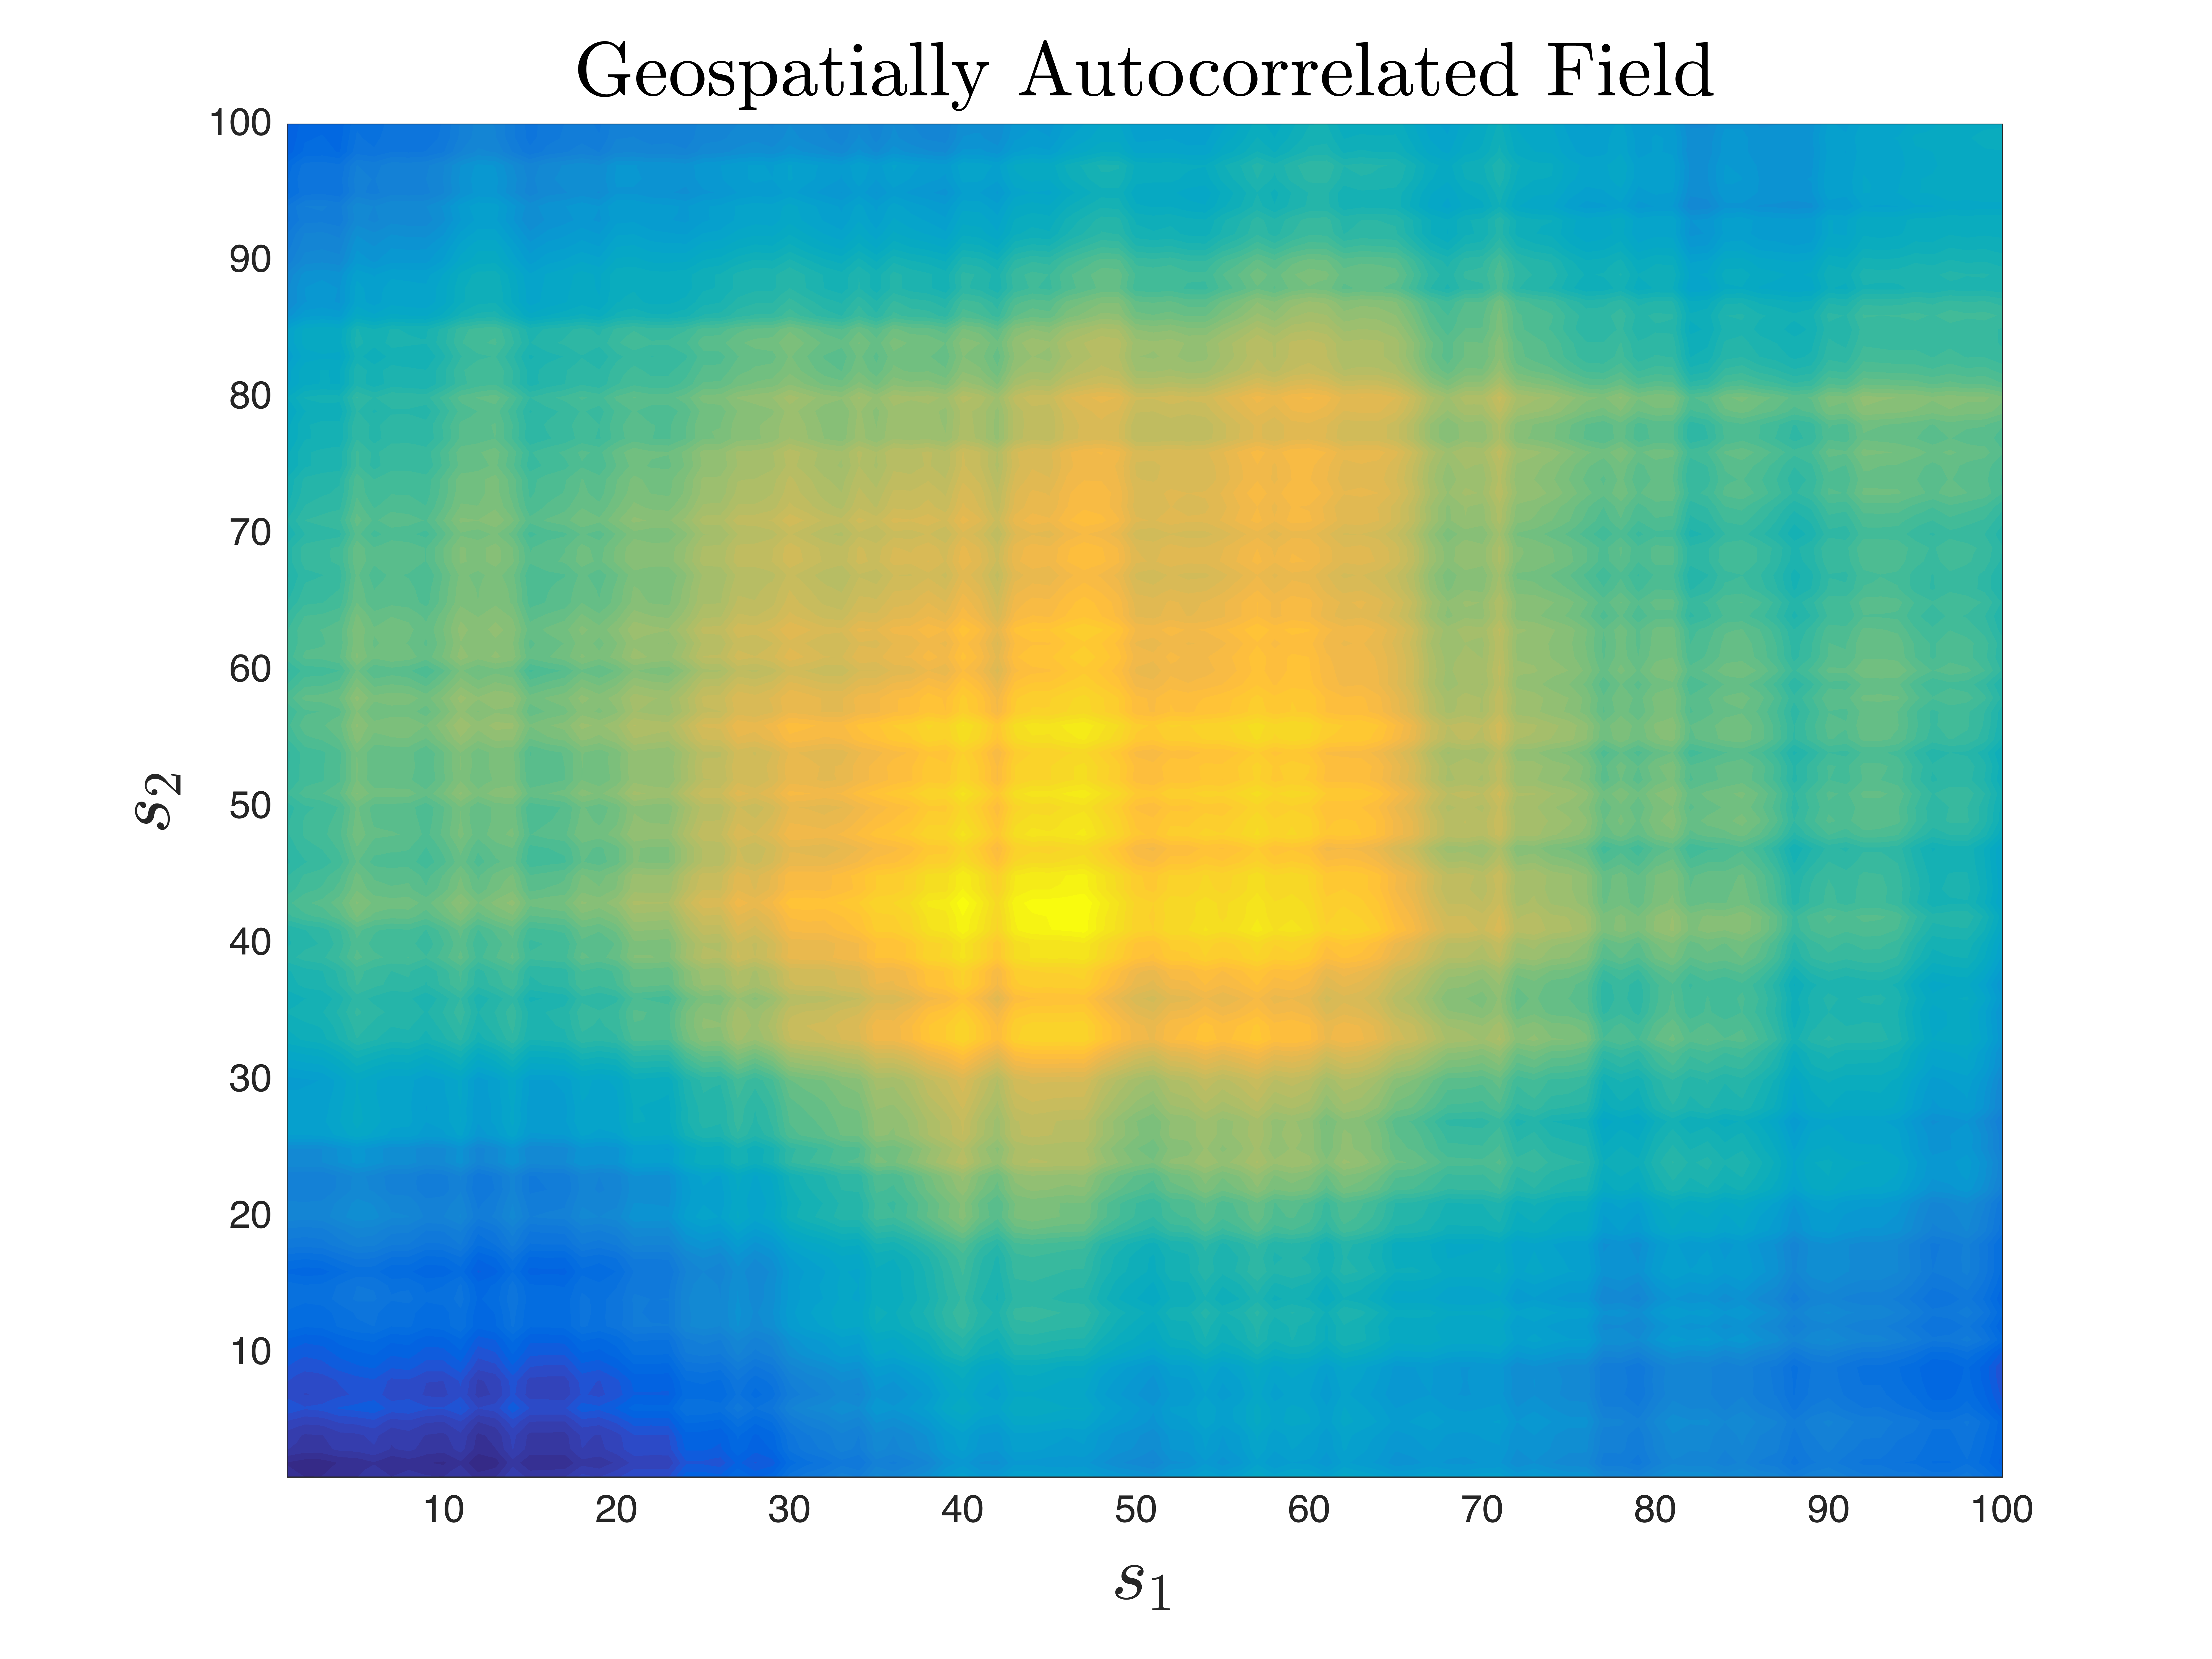
\includegraphics[width=\linewidth]{figures/generated_field.png}
        \captionsetup{skip=0.5\baselineskip,size=footnotesize}
        \ssp
        \caption{A randomly generated spatially autocorrelated field.}
		\label{fig:gen_field}
    \end{subfigure}%
    ~ 
    \begin{subfigure}[t]{0.5\textwidth}
        \centering
        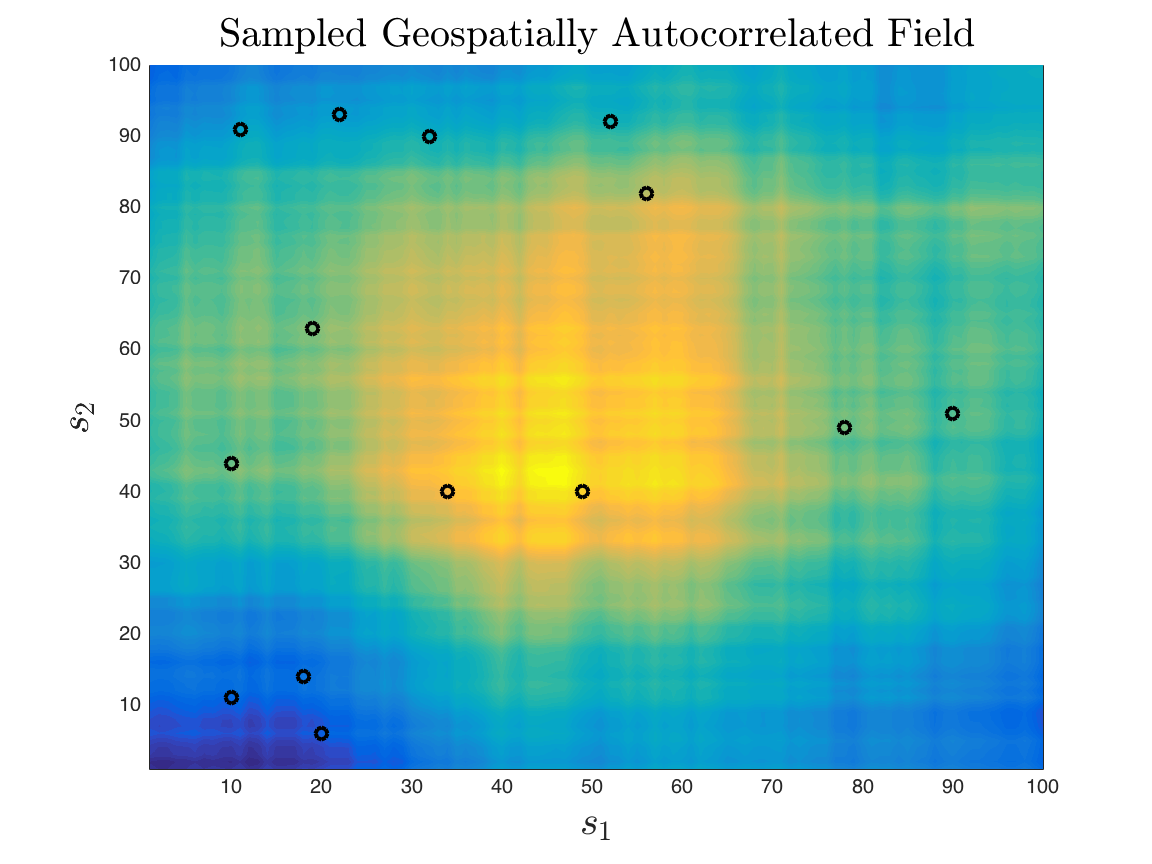
\includegraphics[width=\linewidth]{figures/sampled_generated_field.png}
		\captionsetup{skip=0.5\baselineskip,size=footnotesize}
		\ssp
        \caption{Samples at marked locations were taken of the target field in \ref{fig:gen_field}.}
		\label{fig:sampled_field}
    \end{subfigure}
    \ssp
    \caption{A Gaussian distributed randomly generated spatially autocorrelated field.}
    \label{fig:generated_and_sampled_field}
\end{figure}

\section{Inverse Distance Weighting} \label{sec:idw_intro}
An inverse distance weighting is a naive interpolation tool where a point is predicted based its distances from a set of observed points. A simple IDW, using Shepard's Method \cite{shepard:idw}, gives a prediction, $\hat{Z}(\vect{s}_j)$, of an unobserved point, $\vect{s}_j$, as a function of the $N \in \mathbb{N}$ observed points, $\{Z(\vect{s}_1), Z(\vect{s}_2), \hdots, Z(\vect{s}_n) \}$.

\begin{equation}
	\hat{Z}(\vect{s}_j)=\begin{cases}
			\dfrac{\sum\limits_{i=1}^N [w(\vect{s}_j, \vect{s}_i)] Z(\vect{s}_i) }{\sum\limits_{i=1}^{N} w(\vect{s}_j, \vect{s}_i)} & \text{if}\ \forall i \mid d(\vect{s}_j,\vect{s}_i) \neq 0\ \\
			Z(\vect{s}_j) & \text{if}\ \exists i \mid d(\vect{s}_j,\vect{s}_i)=0\\
		\end{cases}
\end{equation}
\begin{equation}
    d(\vect{s}_j,\vect{s}_{i})=\|\vect{s}_j-\vect{s}_i\|_{2}
\end{equation}
\begin{equation}
	w(\vect{s}_j, \vect{s}_i)=\frac{1}{d(\vect{s}_j,\vect{s}_{i})^{p}}=\|\vect{s}_j-\vect{s}_i\|_{2}^{-p}
\end{equation}

\noindent where $p \in \mathbb{R}^{+}$ is the IDW "power parameter". The power parameter, $p$, controls the emphasis on near and far observations on a prediction. As $p$ increases, the predicted values more closely resemble the closest made observation to the prediction location. Inversely, as $p$ gets smaller within $(0, 1]$, more emphasis is drawn from observations made further away.\\

\begin{figure}[ht!]
    \centering
    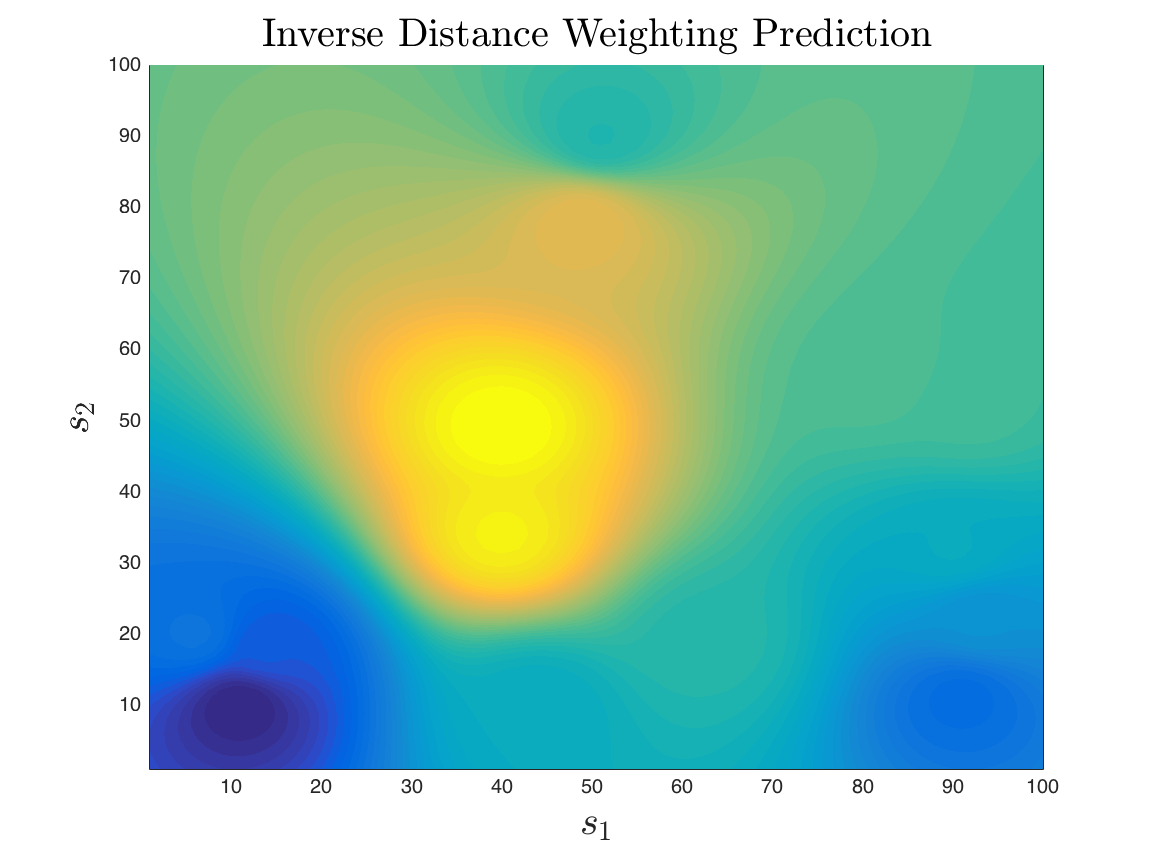
\includegraphics[width=0.8\linewidth]{figures/idw_predicted_field.png}
    \ssp
    \caption{An inverse distance weighting predicted field generated from the samples taken of Figure \ref{fig:gen_field} at the locations marked in Figure \ref{fig:sampled_field}.}
    \label{fig:idw_field}
\end{figure}

This method can yield a prediction for all possible points in a field where a set of observations at known locations are made, as done in Figure \ref{fig:idw_field}. Unfortunately, the method is limited in that it assumes a spherical distribution of correlation of points in a field, and does not take advantage of the underlying spatial correlation patterns of the target field being observed to make a more methodical weighted sum prediction. A field that exhibits properties of spatial autocorrelation would be more statistically exploitable because the distribution of the states of interest on the field can be learned.

\section{Variography} \label{sec:vario}
Variography is a set of procedures for examining and interpreting spatial dependence and spatial autocorrelation in a field of observed data. The \textit{variogram} of a field will be introduced to assist in extracting the underlying spatial autocorrelation function of a target field. The variogram function will be factored into a classical prediction via weighting, yielding a Kriging Weighting.

\subsection{The Variogram}
A variogram quantifies dependence for two disjoint observations separated by some distance, or \textit{lag}, away. The function, in essence, yields a value directly proportional to the covariance between two given points in a stochastic field.

A Variogram is intended to be a continuous function which yields a covariance between two points $Z(\vect{s}_{i})$, $Z(\vect{s}_{j})$, which have not necessarily been observed, but known to be a Euclidean distance, or lag, $h_{i,j} \in \mathbb{R}$ apart \cite{deutsch:geostat}, where

\begin{equation}
h_{i,j} = \| \vect{s}_i - \vect{s}_j \|_2
\label{eq:hdist}
\end{equation}

Using the assumption on what a point's value on a field is constructed of is made in Equation 2.4.1 of Matheron, 1963 \cite{matheron:geostat}:

\begin{equation}
    Z(\vect{s}_i)=\mu(\vect{s}_i)+\theta(\vect{s}_i)
    \label{eq:matheron:assum}
\end{equation}

\noindent where $\theta(\cdot)$ is a zero-mean intrinsically stationary stochastic Wiener process, and $\mu(\cdot) = \bar{Z}$ is the mean value of the state of interest in the field.

\subsection{The Semivariogram}
The Semivariogram is defined to be the average squared difference between two points separated by some distance apart. Matheron, 1963 defines a semivariogram in \cite{matheron:geostat} in three-dimensional space as:

\begin{equation}
    \gamma(h) = \frac{1}{2A} \iint_A [ Z(\vect{s} + h) - Z(\vect{s}) ]^2 dA
    \label{eq:semivariogramint}
\end{equation}

\noindent where $A$ is a closed area in a field to consider, $Z(\vect{s})$ is the value of a point at location $\vect{s}$ on the field, and $Z(\vect{s} + h)$ is the value of some point a distance $h$, defined in Equation \ref{eq:hdist}, apart from a point $\vect{s}$ on the field.

It is infeasible to estimate an observation value at each possible point in the field to compute a continuous Semivariogram. Furthermore, the fields observed using these methods are typically gridded, and therefore not continuous by their analytical nature. A discrete model must first be constructed, and will then be fit into a continuous variogram model. This is done by first constructing a discrete variogram model, or \textit{Empirical Semivariogram}, and then fitting a continuous model to it. Fitting a discrete Semivariogram should in turn yield a function close to $\gamma(h)$ defined in Equation \ref{eq:semivariogramint}, and should be identical assuming every point in the area $A$ is sampled with infinite precision.

\subsection{The Empirical Semivariogram}
An Empirical Semivariogram, or Experimental Semivariogram, is a discrete function representing the covariance of the observation value difference between two sampled locations that are some distance $h$ apart. Goovaerts defines the empirical variogram in \textit{Geostatistics for Natural Resources Evaluation. Applied Geostatistics Series} \cite{goov:97} as:

\begin{equation}
    \label{eq:exp_var}
    \hat{\gamma}(h) = \frac{1}{2N(h)}\sum_{i=1}^{N(h)} (Z(\vect{s}_i) - Z(\vect{s}_i+h))^2
\end{equation}

\noindent where $N(h)$ is the cardinality of the set of all pairs of observed points that are a Euclidean distance, or lag, $h$, apart.

The experimental variogram conveys the spatial autocorrelation of a sampled field. As the lag between two given points increases, the covariance also increases when the field is spatially autocorrelated. The covariance levels out to a steady value (the \textit{sill}) at some distance in the domain (the \textit{range}). The range marks the point where the loss of reliable spatial autocorrelation between two points ceases.

\begin{figure}[ht!]
    \centering    
    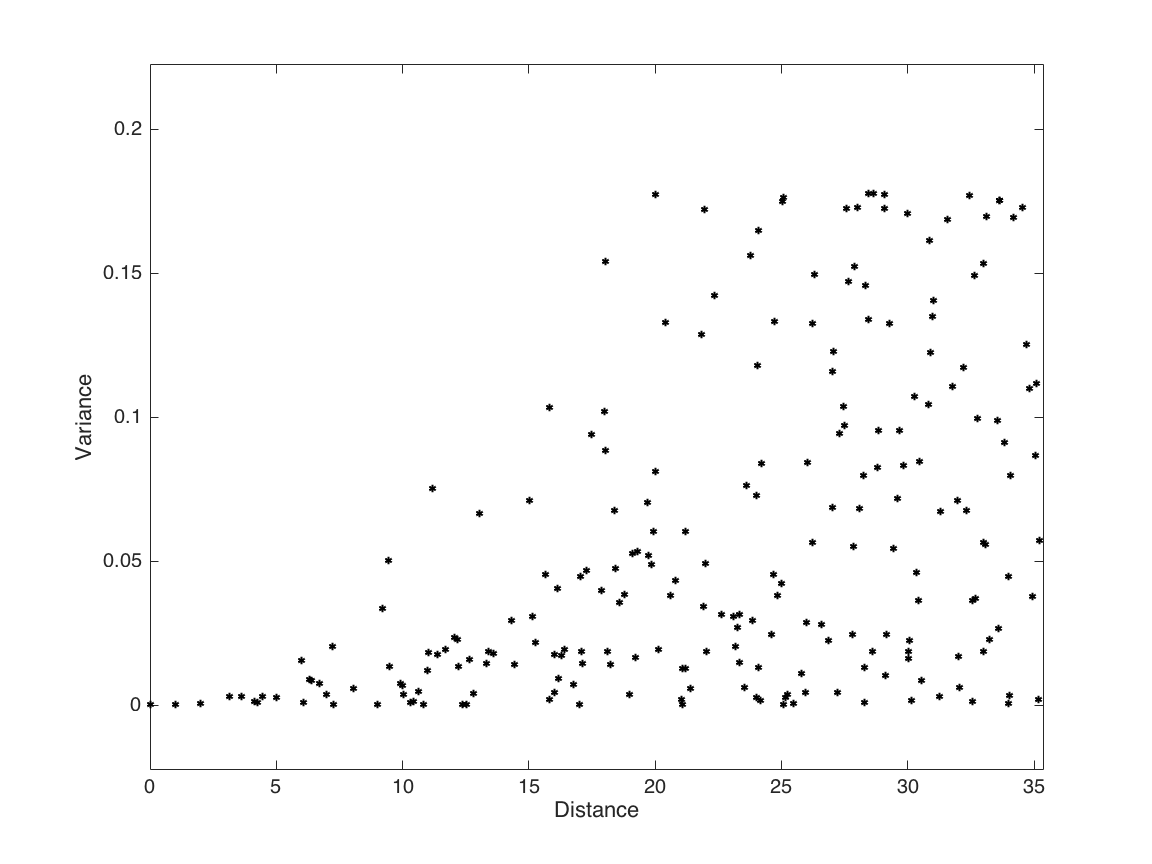
\includegraphics[width=0.8\linewidth]{figures/exp_variogram.png}
    \ssp
    \caption{An empirical semivariogram.}
    \label{fig:emp_semiv}
\end{figure}

\subsection{Converting a Semivariogram to a Variogram} \label{sec:semitovar}
The intent of fitting a statistical model to an experimental variogram is to approximate the continuous covariance for any two points, that have not necessarily been observed, on $Z$ that are at some known lag apart.

The Empirical Semivariogram will be fit to a statistical model, or \textit{kernel}, known as a Variogram Model. There exist well-known models, further discussed in this section. Each model is a scalar function of lag, $h$, \text{sill}, $s$, and \text{range}, $a$. The term \textit{sill} refers to the point on the co-domain where two points at the lag specified are no longer autocorrelated. The sill is therefore the largest value of covariance for two disjoint points on a field that are still considered to be autocorrelated. The corresponding point on the domain for the sill is referred to as the \textit{range} on the variogram. Two points that have a lag larger than the range are not considered to be autocorrelated. The \textit{nugget} of the variogram is defined to be the variance at zero lag, or $\gamma(0)$ \cite{matheron:geostat}. This value is exactly zero for ideal measurements. For non-ideal situations, the nugget is typically non-zero. This can be attributed to drift in the the field states between sampling periods, or from measurement noise. The value found for the nugget is summed with the value yielded by $\gamma$, to get the final variogram value for a given lag \cite{goov:97}.

\subsubsection{The Gaussian Model}

\begin{equation}
	\gamma_g(h, s, a) = s \Bigg[ 1 - \exp \Bigg( -\dfrac{h^2}{a^2} \Bigg) \Bigg]
	\label{eq:gauss_model}
\end{equation}

The Gaussian model will asymptotically reach its sill. The sill would be at the limit as $h$ approaches infinity. The \textit{practical range} is therefore used to refer the point on the domain where the variogram reaches 95\% of its sill \cite{goov:97}.

\subsubsection{The Exponential Model}

\begin{equation}
	\gamma_e(h, s, a) = s \Bigg[ 1 - \exp \Bigg( \dfrac{h}{a} \Bigg) \Bigg]
	\label{eq:exp_model}
\end{equation}

The same rules as the Gaussian model apply to the Exponential model \cite{goov:97}.

\subsubsection{The Spherical Model}

\begin{equation}
	\gamma_s(h, s, a) = \frac{s}{2} \Bigg[ \dfrac{3h}{a} - \Bigg( \dfrac{h}{a} \Bigg)^3 \Bigg]
	\label{eq:sph_model}
\end{equation}

The spherical model will reach an exactly zero slope at the sill and range \cite{goov:97}.

\begin{figure}[htb!]
    \centering    
    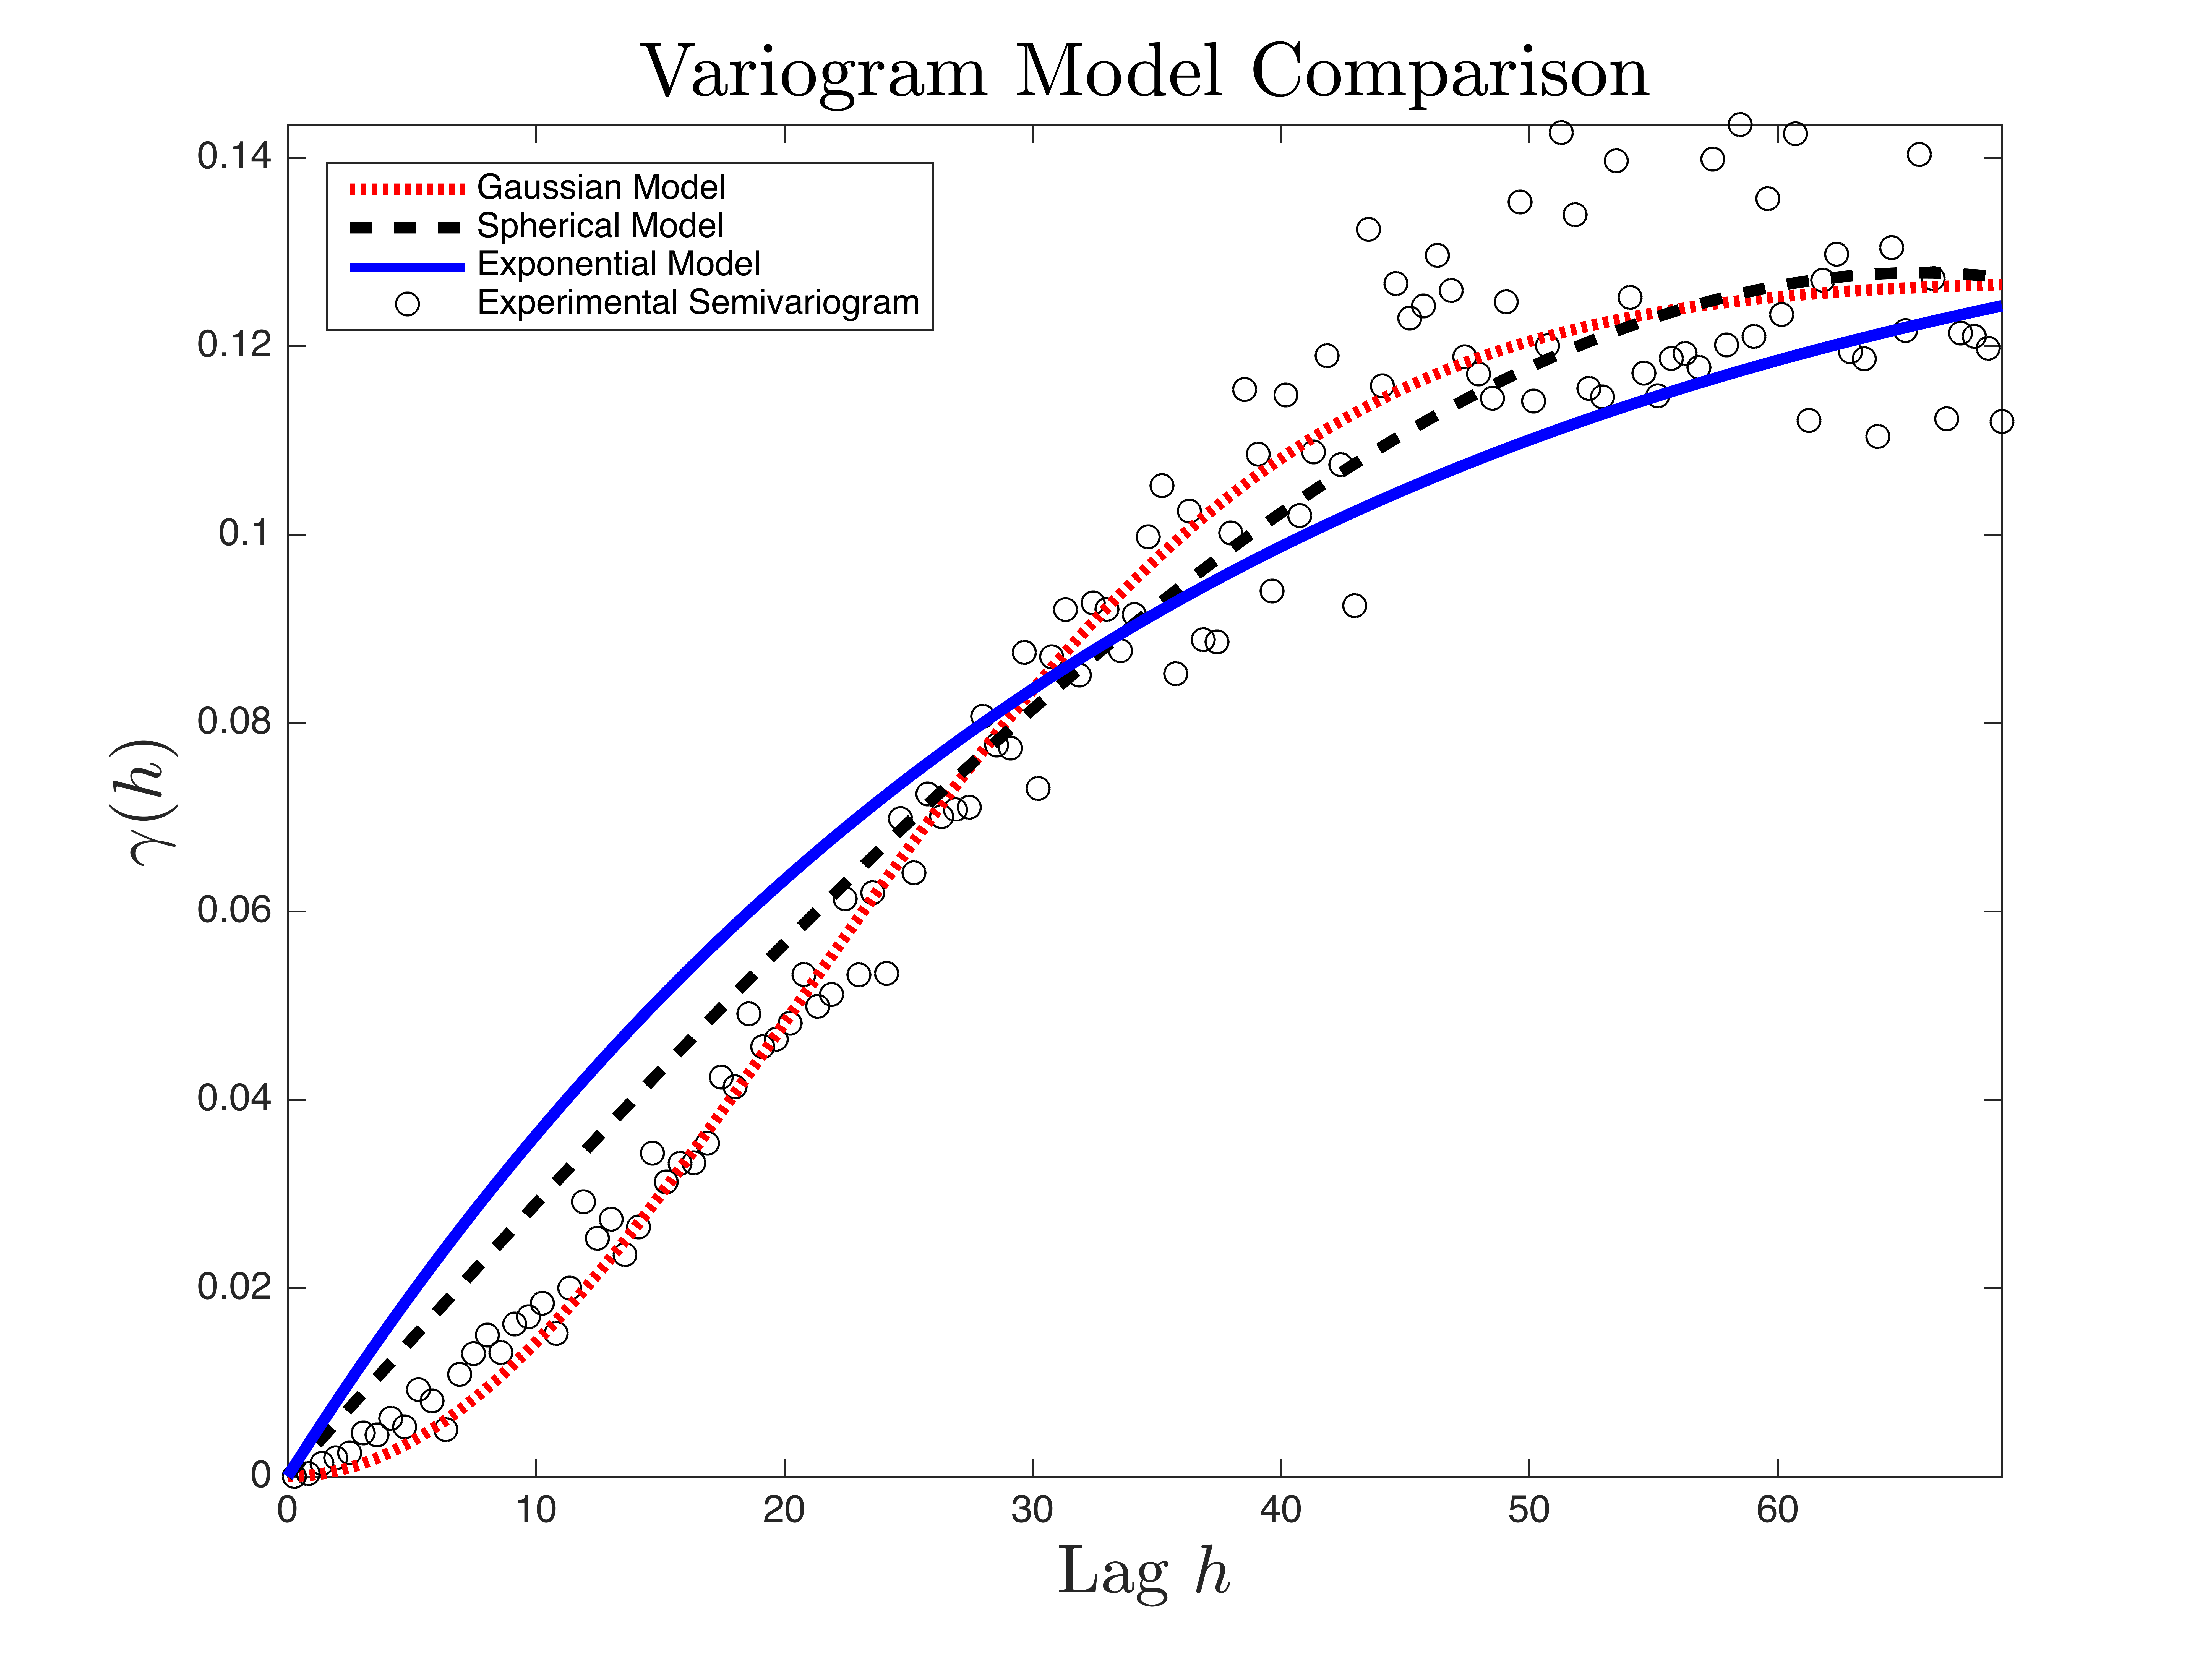
\includegraphics[width=0.8\linewidth]{figures/fit_kern_comp.png}
    \ssp
    \caption{Examples of three different variogram models.}
    \label{fig:fit_kernel_cop}
\end{figure}

\subsection{Fitting A Semi-Variogram} \label{sec:varfit}
The kernel function of the range, $a$, the sill, $s$, and lag, $h$ is chosen based on the statistical properties of the field being examined. Although there exist no closed form solution for finding an appropriate variogram model for a given field, one can compare a variety of different models against one another. Conducting cross-validation tests and comparing root-mean squared prediction errors for different models are common approaches for finding appropriate variogram models.

Using a version of the \textit{fminsearch} function in \textit{MATLAB}, a variogram can be fit to the desired objective function from a set of samples and initial guesses for the range and sill using a simplex search method. As the function is used over several iterations of sampling, the fit range and sill values found in the previous iteration can be used as the seed to the next iteration of the fit in an attempt to minimize computation time. The \textit{MATLAB} function, \textit{fminsearch}, is defined to ``find the minimum of an unconstrained multi-variable function using a derivative-free method" \cite{mathworks:fminsearch}, expressed in Equation \ref{eq:matlabfmin}.

\begin{equation}
    \gamma(h) = \min\ [\gamma_{kernel}(h,s,a) - \hat{\gamma}(h)]^2
    \label{eq:matlabfmin}
\end{equation}

\noindent The function is then modified by specifying bounds of minimization in an attempt to decrease iterations of the function fit, which can be computationally expensive as more samples are taken. This modified version of \textit{fminsearch}, named \textit{fminsearchcon}, can be downloaded from the MathWorks File Exchange.

\begin{figure}[ht!]
    \centering    
	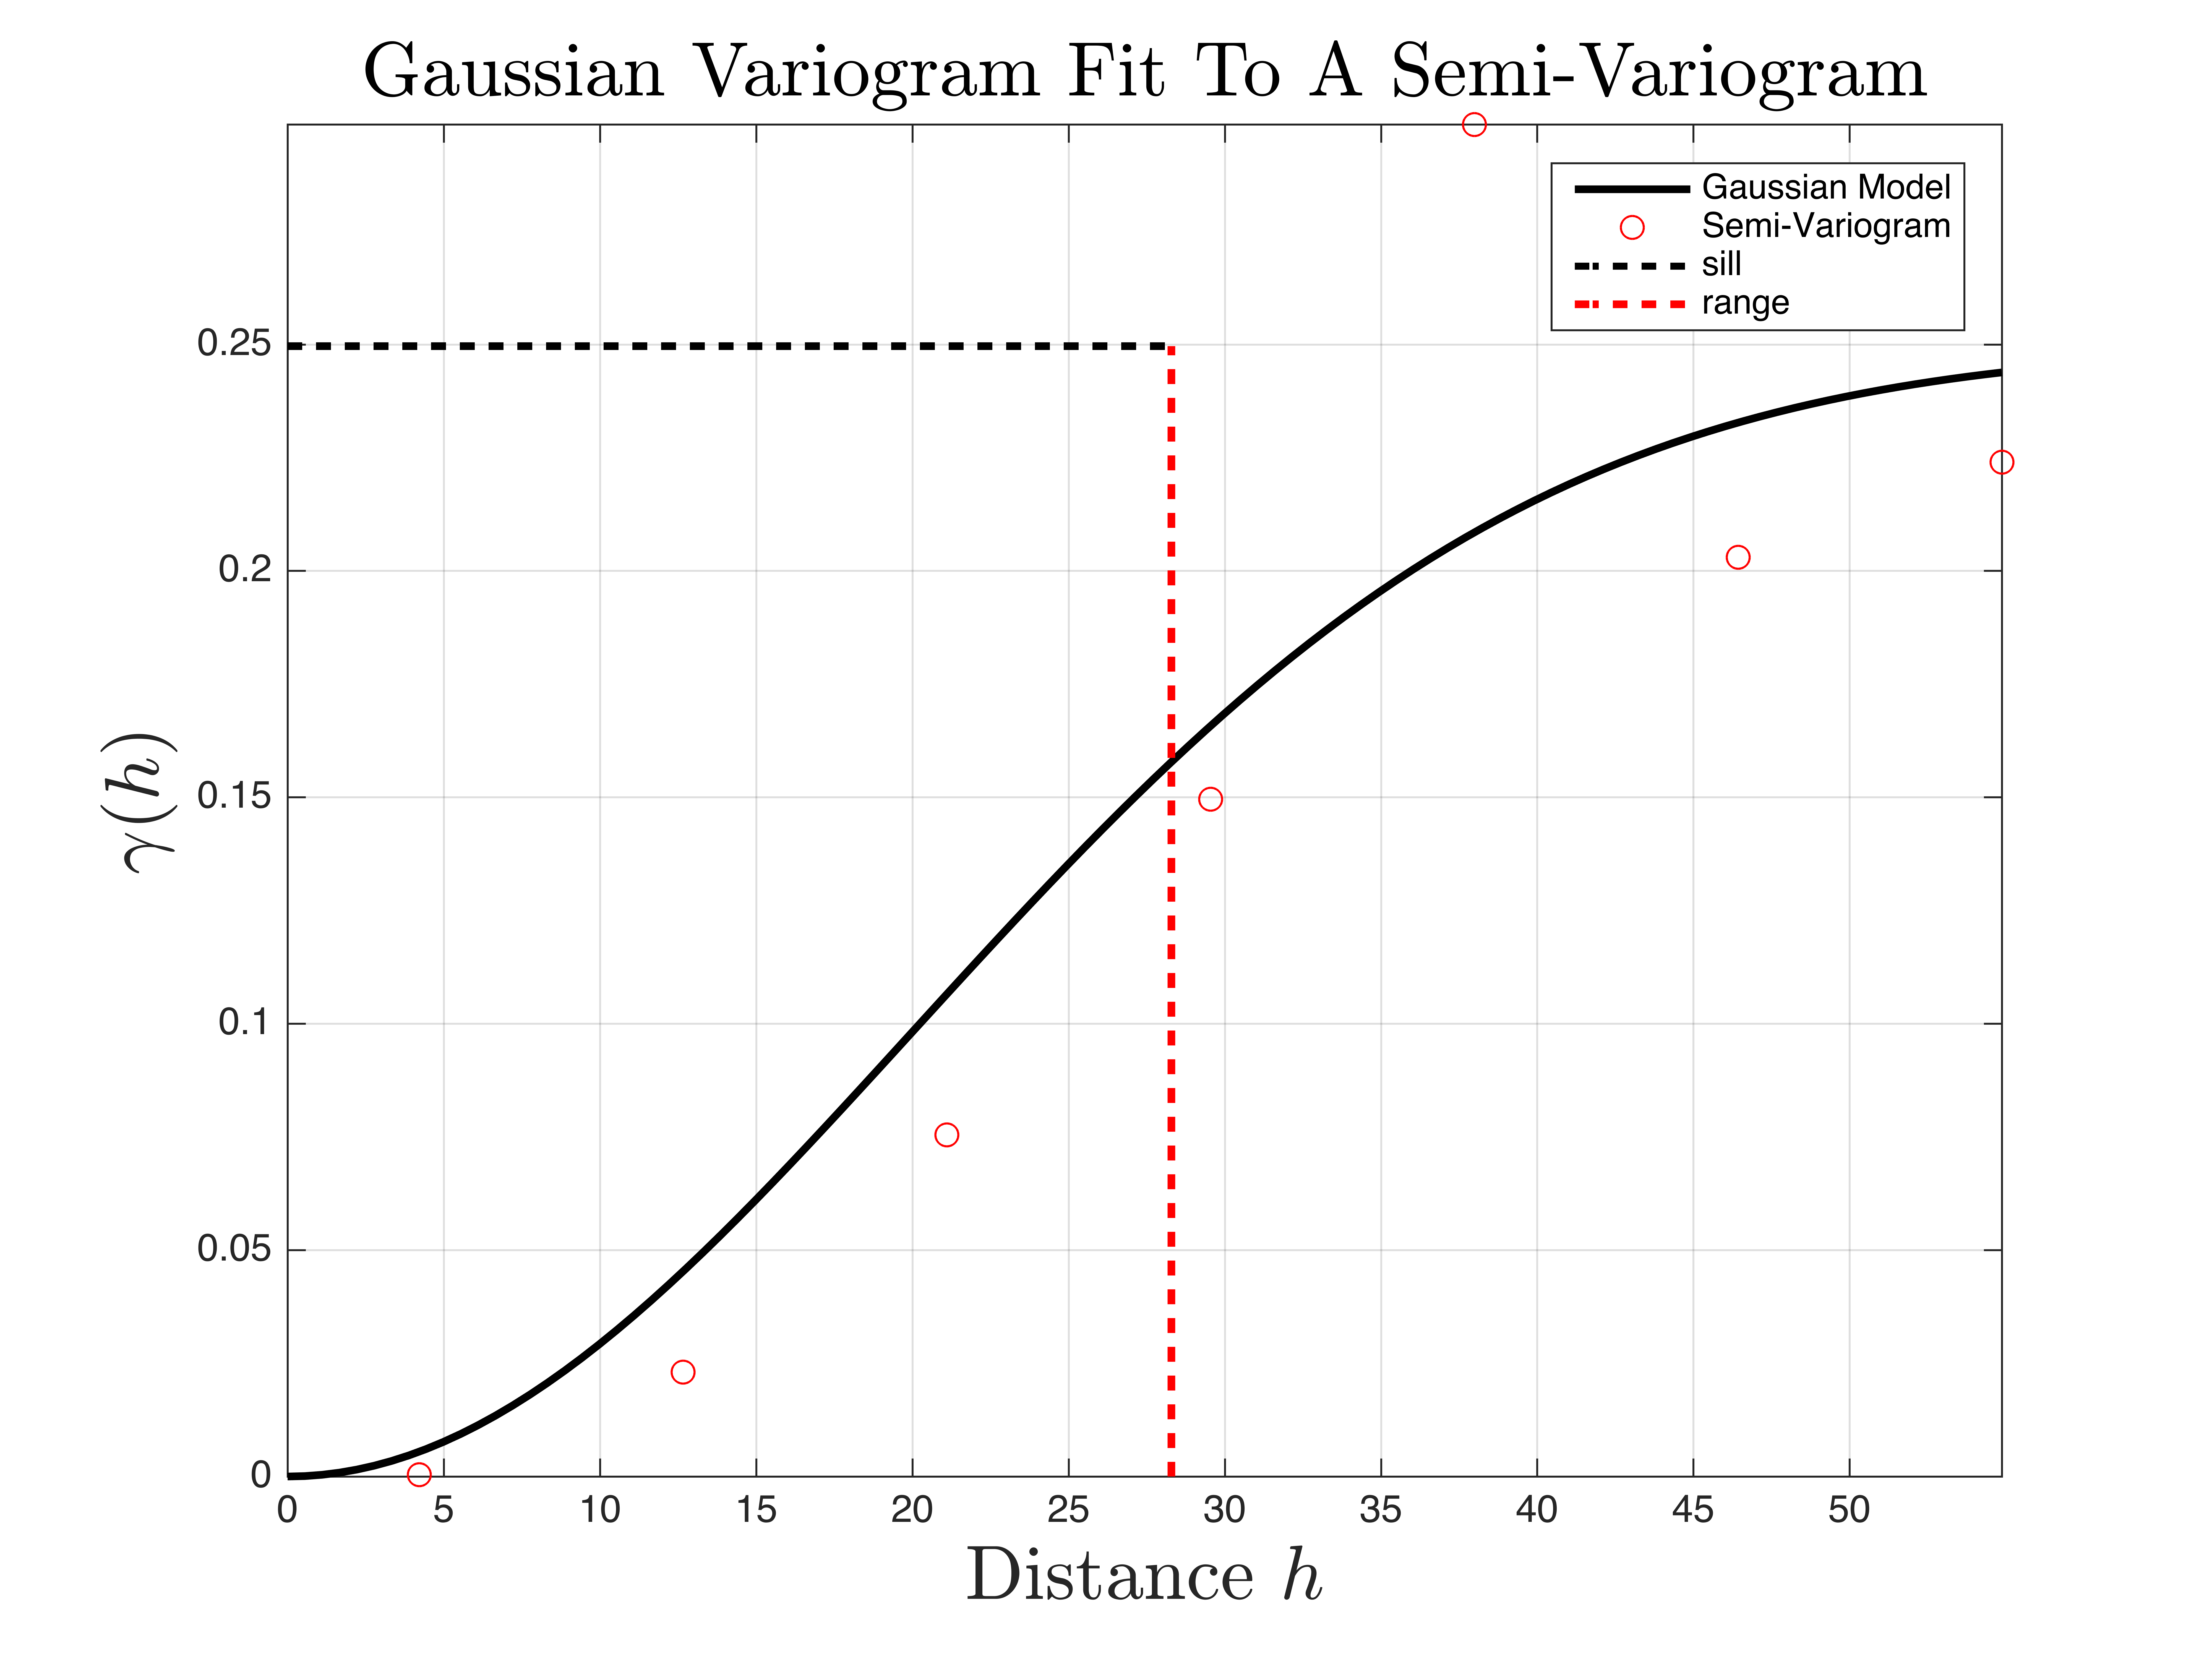
\includegraphics[width=0.8\linewidth]{figures/fit_kernel.png}
    \ssp
	\caption{An experimental variogram generated using Equation \ref{eq:exp_var} from the samples taken in Figure \ref{fig:sampled_field}. $\delta$ was chosen such that for $n$ observations, a total number of $\Big\lfloor \frac{n}{2} \Big\rfloor$ points were plotted. A Gaussian statistical model was fit to the experimental variogram. The variogram was fit using \textit{fminsearchcon} in \textit{MATLAB}.}
	\label{fig:fit_kernel}
\end{figure}

\section{The Kriging Method}
The Kriging Method conducts a weighted sum using the continuous variogram model that was fit to the physical observations made. The method can yield a prediction for each vesicle in a target space similar to the Inverse Distance Weighting method described in Section \ref{sec:idw_intro}, but with more statistical robustness.

\subsection{Forms of the Kriging Method}
There exist three major forms of the Kriging Method; all of which differ primarily in the handling of the mean gathered from observations of a target field. The \textit{Simple Kriging Method} makes the assumption that the mean is known and constant throughout the entirety of an observed field. This is not the case for fields that are very large as it does not follow Tobler's First Law. The \textit{Ordinary Kriging Method} can deduce the local mean of a neighborhood from a smaller subset of observations in a larger target field. This is done by classifying the larger field into smaller neighborhoods where the mean is only constant within those neighborhoods. Ordinary Kriging has the advantage that the mean is not required to be known before running a prediction. The \textit{Universal Kriging Method} can perform similar local mean calculations as the Ordinary Kriging Method, but does so by fitting a polynomial representing a mean trend model and not from a constant mean value representing that neighborhood \cite{vandergraaf:nnkrig} as seen in Section \ref{sec:varfit} on fitting a variogram. The Ordinary Kriging method will be used throughout the rest of this thesis because of its lack of requirement for the expected value of the field, and its computational simplicity when compared to the Universal Kriging Method.

\subsection{Covariance Matrix From A Variogram} \label{sec:covmat}
From the fit variogram which represents the spatial statistics of a field from a set of samples, a variance-covariance matrix for $N$ observations, $P \in \mathbb{R}^{N \times N}$, will be constructed. The value of the element $P_{i,j}$, will represent the covariance of the lag between the $i^{th}$ and $j^{th}$ observations on the field \cite{goov:97}, \cite{matheron:geostat}. If $i=j$, the value of the element, $P_{i,j}$ is the variance of the $i^{th}$ observation. 

\begin{equation}
    P_{i,j} = \text{cov}\{Z(\vect{s}_{i}), Z(\vect{s}_{j})\} = \gamma(\| \vect{s}_i - \vect{s}_j \|_2)
    \label{eq:covvarmatelem}
\end{equation}

\begin{equation}
    P = \begin{bmatrix} 

    \gamma(0) & \gamma(\| \vect{s}_1 - \vect{s}_2 \|_2) & \dots & \gamma(\| \vect{s}_1 - \vect{s}_N \|_2)\\
    
    \gamma(\| \vect{s}_2 - \vect{s}_1 \|_2) & \gamma(0) & \dots & \gamma(\| \vect{s}_2 - \vect{s}_j \|_N)\\

    \vdots & \vdots & \ddots & \vdots \\
    
    \gamma(\| \vect{s}_N - \vect{s}_1 \|_2) & \gamma(\| \vect{s}_N - \vect{s}_2 \|_2) & \dots & \gamma(0)\\

    \end{bmatrix}
    \label{eq:covvarmat}
\end{equation}

\subsection{Mean \& Variance of a Point Prediction}
For any given point on a field, we can construct a \textit{proximity vector}, $\vect{d}_0 \in \mathbb{R}^{N}$, which contains the covariance of a given point, $\vect{s}_0$ on the field with the $N$ observations made. The $k^{th}$ element of $\vect{d}_N$, would therefore contain the covariance for the lag between point $\vect{s}_0$ and the $k^{th}$ observation made, $\vect{s}_k$ \cite{matheron:geostat}.

$$\vect{d}_0(k) = \gamma(\| \vect{s}_0 - \vect{s}_k \|_2)$$

\begin{equation}
    \vect{d}_0 =
        \begin{bmatrix} 
                    \gamma(\| \vect{s}_0 - \vect{s}_1 \|_2) \\
                    \gamma(\| \vect{s}_0 - \vect{s}_2 \|_2) \\
                     \vdots \\
                    \gamma(\| \vect{s}_0 - \vect{s}_N \|_2) \\
        \end{bmatrix} 
    \label{eq:proxvect}
\end{equation}

\noindent Furthermore, The Kriging Method can be bounded. If a to-be-predicted point and a given sample is beyond the range value fit to the variogram model, the corresponding element in the proximity vector is set to the sill. This ensures that points outside of the range of autocorrelation are not weighted anymore than they should be. This method is suggested when the variogram model used is a bounded function, e.g. the Spherical Model (Equation \ref{eq:sph_model}).

A set a weights will be computed for each vesicle in the target field similarly to the Inverse Distance Weighting method. These weights will be referred to as the \textit{Ordinary Kriging Weights}. For a given prediction location, $\vect{s}_0$, the Ordinary Kriging Weight vector, $\vect{\lambda}_0$, will be defined as the product of the inverse of the covariance matrix of the field and the proximity vector of the point to predict \cite{felus:srn}.

\begin{equation}
    \begin{bmatrix}
    \vect{\lambda}_{0} \\
    \eta_0
    \end{bmatrix} = \begin{bmatrix} P^{-1} & \vect{1} \\
                                    \vect{1}^T & 0 \end{bmatrix}
                                    \begin{bmatrix} 
                                    \vect{d}_{0} \\
                                    1
                                    \end{bmatrix}
    \label{eq:krigweights}
\end{equation}

\noindent where $\eta_0$ is a Lagrangian multiplier and $\vect{1} \in \mathbb{R}^{N}$ is a vector of $1$s. These terms assist the Ordinary Kriging system in maintaining unbiasedness in predictions by forcing the sum of the Kriging Weights, $\lambda_0$, to zero \cite{felus:srn}. 

The Ordinary Kriging equation will be used to predict the value, $\hat{Z}(\vect{s}_0)$ of an unobserved location, $\vect{s}_0$. The prediction is a function of the Kriging Weights and a vector of $N$ observations \cite{felus:srn}. 

\begin{equation}
    \hat{Z}(\vect{s}_0) = \begin{bmatrix} Z(\vect{s}_1) & Z(\vect{s}_2) & \dots & Z(\vect{s}_N) \end{bmatrix}\vect{\lambda}_{0}
    \label{eq:krigeq}
\end{equation}

\begin{figure}[!]
    \centering
    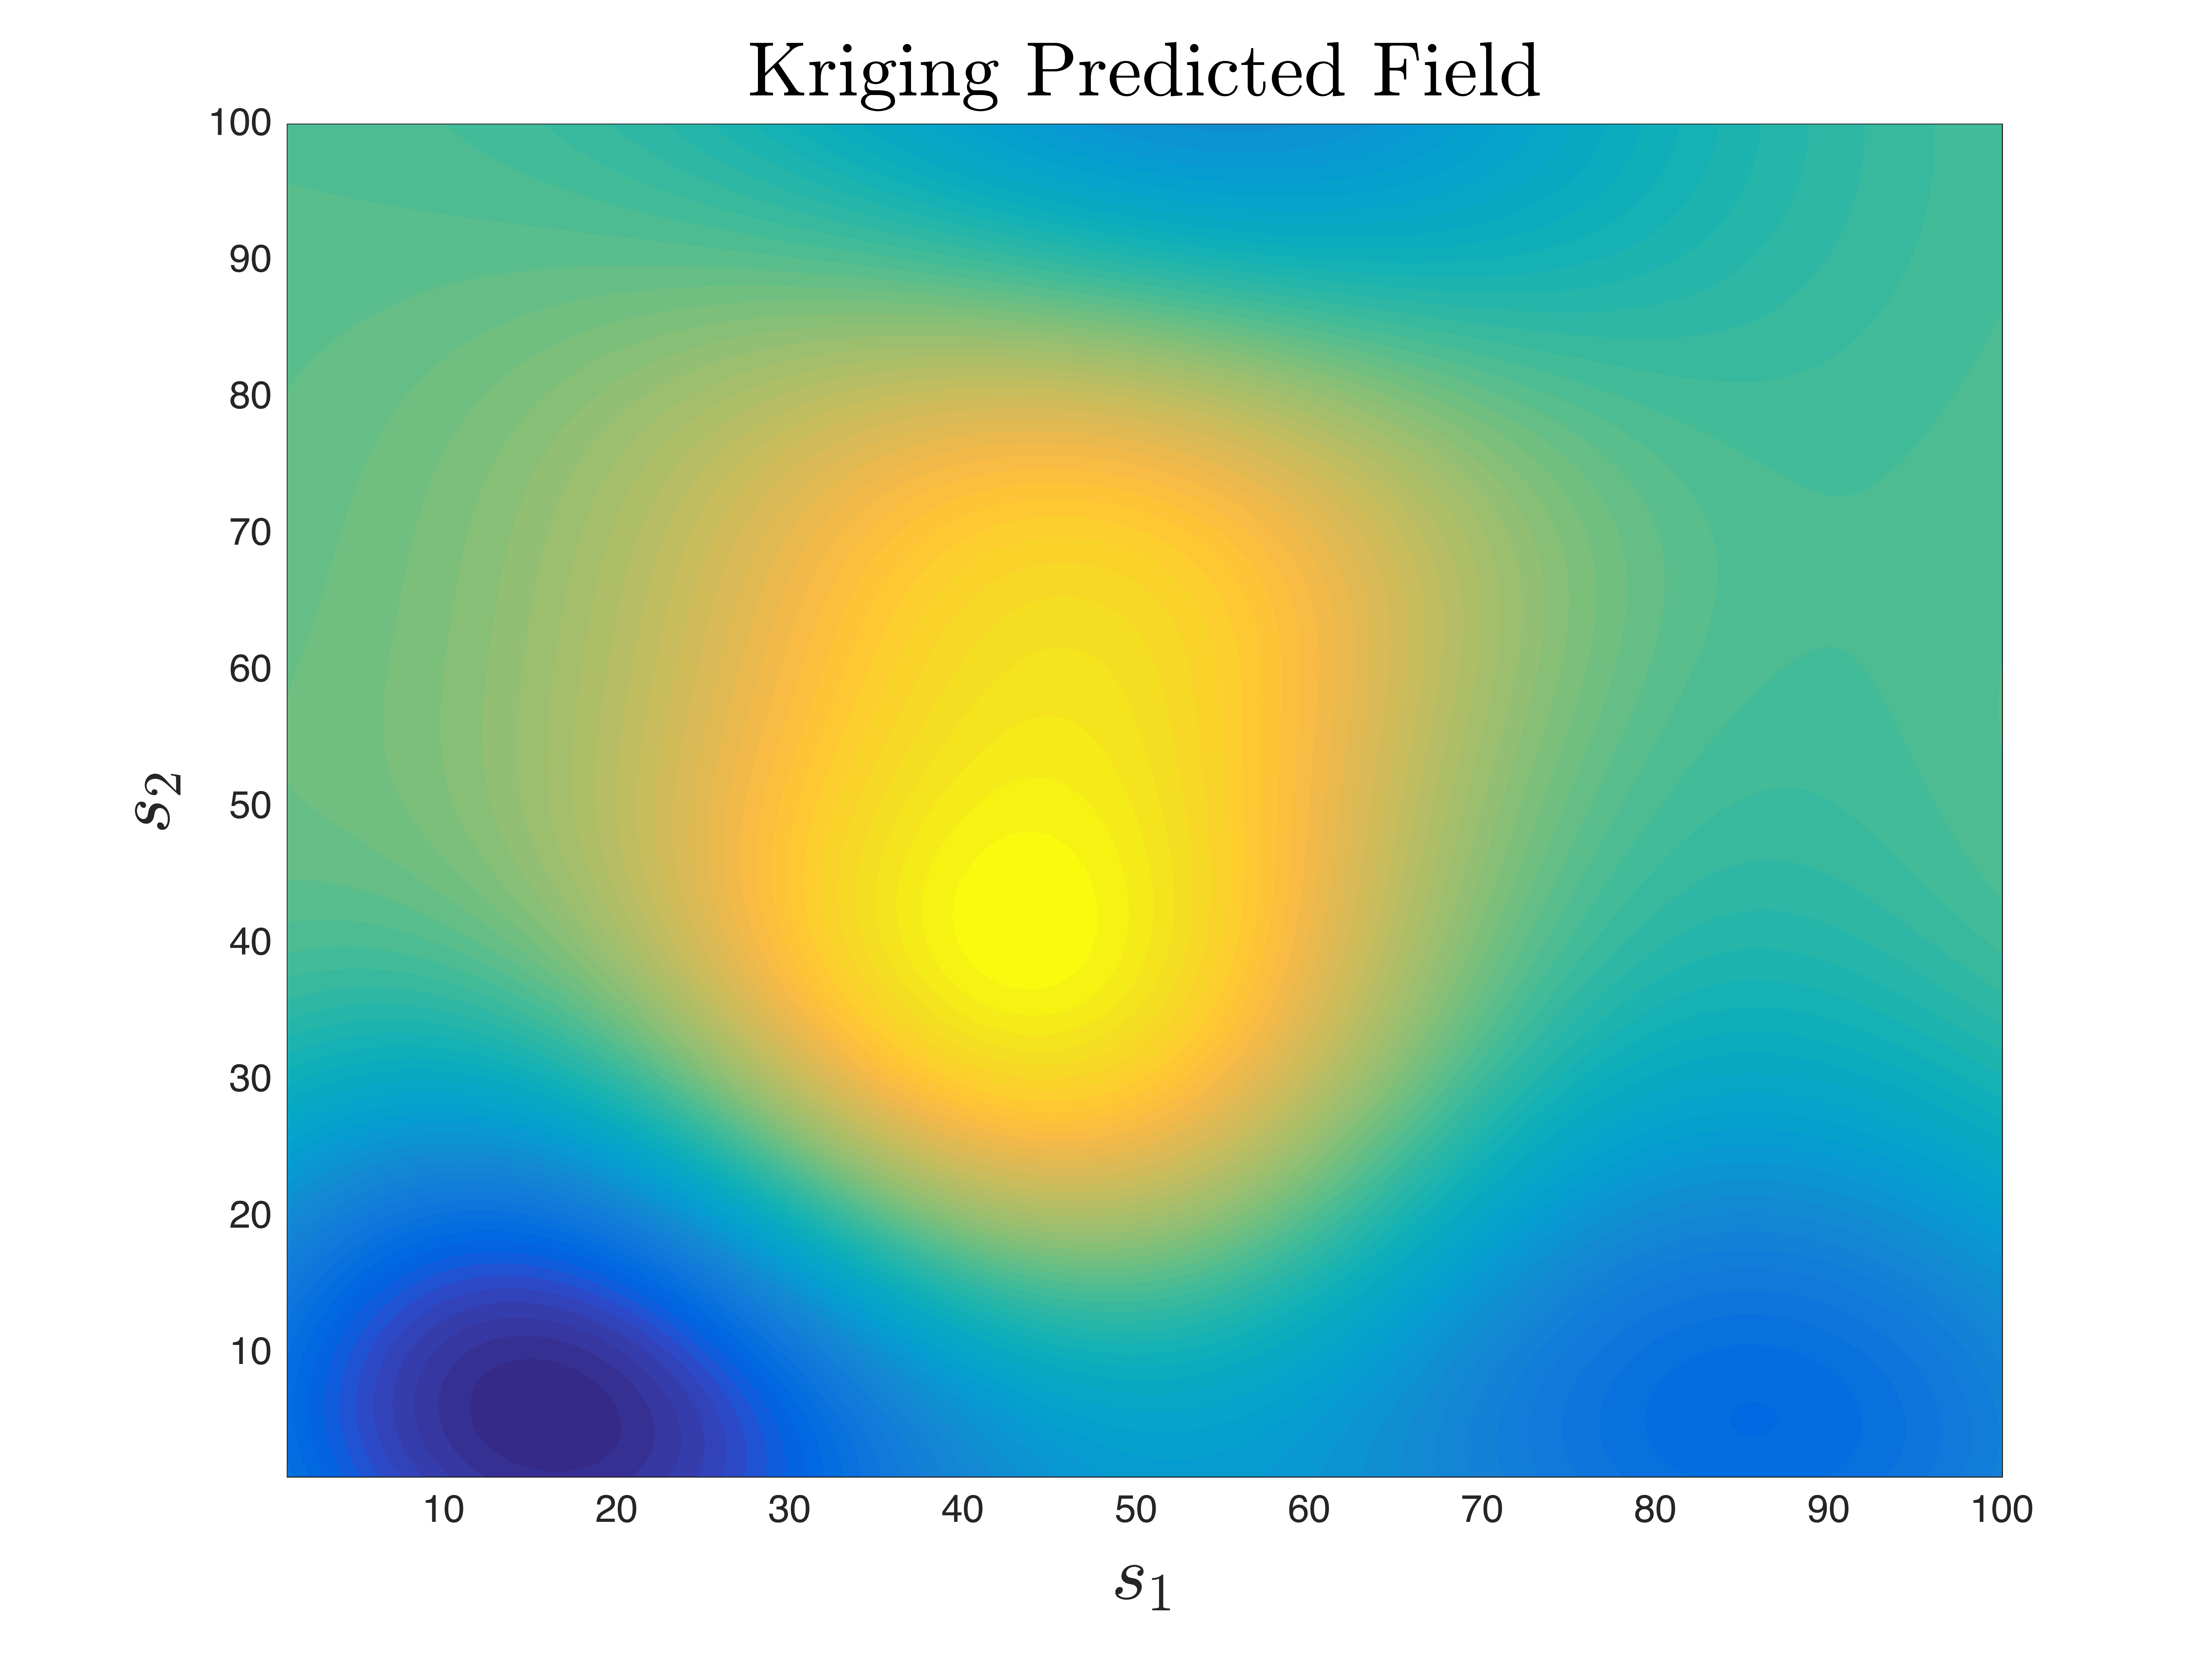
\includegraphics[width=0.8\linewidth]{figures/kriging_prediction.png}
    \ssp
    \caption{A Kriging Method predicted field generated from the samples taken of Figure \ref{fig:gen_field} at the locations marked in Figure \ref{fig:sampled_field}.}
    \label{fig:krig_field}
\end{figure}

The variance of a point predicted on a target field can be calculated using byproduct terms generated along the way of calculating a Kriging prediction \cite{felus:srn}. For a predicted point $\hat{Z}(\vect{s}_0)$, using the proximity vector, $\vect{d}_0$, defined in Equation \ref{eq:proxvect}, and the Kriging Weights, $\vect{\lambda}_0$ defined in Equation \ref{eq:krigweights} for the predicted point, the variance of the prediction for that point is defined as:

\begin{equation}
    \label{eq:krigvar}
    \text{var}\{\hat{Z}(\vect{s}_0)\} = \begin{bmatrix}\vect{d}_0 \\ 1\end{bmatrix} \begin{bmatrix}\vect{\lambda}_0^T & \eta_0 \end{bmatrix}
\end{equation}

\subsection{Procedure For Field Prediction Using The Kriging Method}
The Kriging Prediction is run at every possible unobserved vesicle in the target field in order to predict the entirety of a target field from a finite set of $N$ observations and their respective locations, $O$.

\begin{algorithm}[thpb!]
\caption{Kriging Prediction of Target Field}\label{alg:krig}
\begin{algorithmic}[1]
\Procedure{KrigingPredictField}{$Z$, $O$}
\BState \emph{Generate Semi-Variogram}:
\State $\forall$ $\vect{s}_i$, $Z(\vect{s}_i)$ $\in O$:
\State \ \ \ \ $\hat{\gamma}(h) \gets \vect{s}_i$, $Z(\vect{s}_i)$\\
\BState \emph{Generate Variogram}:
\State $\gamma(h)$ fits to $\hat{\gamma}(h)$\\
\BState \emph{Construct Covariance Matrix}:
\State $\forall (\vect{s}_i,\vect{s}_j) \in O:$
\State \ \ \ \ $h_{i,j} = \|\vect{s}_i - \vect{s}_j\|_2$
\State \ \ \ \ $P_{i,j} = \gamma(h_{i,j})$\\
\State $\forall i \in [1, N]:$
\State \ \ \ \ $P_{i,N+1} = 1$
\State \ \ \ \ $P_{N+1,i} = 1$
\State $P_{N+1,N+1} = 0$\\
\BState \emph{Run Kriging Predictions For Target Field}:
\State $\forall$ $\vect{p}_i \in$ \textit{field}:
\State \ \ \ \ $\vect{d}_{i} = \begin{bmatrix} \gamma(\| \vect{s}_1 - \vect{p}_i \|_2) \dots \gamma(\| \vect{s}_N - \vect{p}_i \|_2) & 1\end{bmatrix}^T$
\State \ \ \ \ $\begin{bmatrix}
                \vect{\lambda}_{\vect{p}_i} \\
                \eta_{\vect{p}_i}
                \end{bmatrix} = \begin{bmatrix} P^{-1} & \vect{1} \\
                                    \vect{1}^T & 0 \end{bmatrix}
                                    \begin{bmatrix} 
                                    \vect{d}_{\vect{p}_i} \\
                                    1
                                    \end{bmatrix}$
\State \ \ \ \ $\hat{Z}(\vect{p}_i) = \begin{bmatrix} Z(\vect{s}_1) \dots Z(\vect{s}_N) \end{bmatrix} \lambda_{\vect{p}_i}$
\State \ \ \ \ $\text{var}\{\hat{Z}(\vect{p}_i)\} = \begin{bmatrix}\vect{d}_i \\ 1\end{bmatrix} \begin{bmatrix}\vect{\lambda}_{\vect{p}_i}^T & \eta_{\vect{p}_i} \end{bmatrix}$
\EndProcedure
\end{algorithmic}
\end{algorithm}

When Algorithm \ref{alg:krig} is run on the target field from Figure \ref{fig:gen_field}, for the samples taken in Figure \ref{fig:sampled_field}, a prediction of the entire field can be generated, as seen in Figure \ref{fig:krig_field}.

\part{Autonomous Field Exploration Using The Kriging Method}
\chapter{Vehicle \& Information Gain Model}
In an effort to formalize the dynamics of the exploration vehicle, and the information gain on the field, the models for vehicle dynamics and field variances will be introduced.

\section{Exploration Vehicle Model Dynamics} \label{sec:vehicledynamics}
The state vector of the vehicle will be defined as follows:
\begin{equation}
\vect{X} = \begin{bmatrix}
	x \\
	y \\
	\theta \\
	V
\end{bmatrix}
\label{eq:vehiclemodel}
\end{equation}

\noindent where $x$ and $y$ are the vehicle's position on a field, $\theta$ is the vehicle's heading angle, $\omega$ is the vehicle's angular velocity, $\dot{\theta}$, and $V$ is the magnitude of the linear velocity of the vehicle. Both $\omega$ and $V$ are control inputs to the vehicle.

The exploration vehicle dynamics will be modeled after a simple forward discrete kinematics model with a constant time step per iteration, $\Delta T$. An iteration of the propagation model will be the sum of the previous iteration, $\vect{X}_{k}$, the nonlinear vehicle dynamics, $\vect{f}(\vect{X}_k)$, and the control input, $\vect{u}_k$.

\begin{equation}
	\vect{X}_{k+1} = \vect{X}_k + \vect{f}(\vect{X}_{k}) + \vect{u}_k
	\label{eq:vehicledynamicsform}
\end{equation}

\begin{equation}
	\vect{X}_{k+1} = \vect{X}_k + \begin{bmatrix}
		V_k \Delta T \cos \theta_k \\
		V_k \Delta T \sin \theta_k \\
		0 \\
		0
	\end{bmatrix} + \begin{bmatrix}
	0 \\
	0 \\
	\theta_k \\
	V_k
	\end{bmatrix}
	\label{eq:vehicledynamicsmodel}
\end{equation}

The speed, $V$, is assumed to be regulated at a constant value for all values of $k$.

\section{Field Uncertainty Model} \label{sec:fielduncert}
In Section \ref{sec:krigvar}, a method for calculating the variance of a prediction was defined as a function of the proximity vector and Kriging weights generated for the prediction point. The variance defined represents the square of the standard deviation of the distribution the expected value of the prediction is sampled from. For points that have been directly measured, the variance is zero, assuming the field has a high level of ergodicity (no drift in the field). The uncertainty of the prediction of a point in the target field is therefore directly proportional to the variance of its prediction. The goal of a path planner intending to suppress uncertainty of predictions in a target field would then be to reduced the overall variance of the target field being explored.

A criterion for overall field uncertainty can be defined as the average variance, calculated from a prediction of a target field from a set $S$ points sampled for all $N$ predictable points on a target field.

\begin{equation}
	\Sigma_{\text{var}}(\hat{Z}_{S}) = \frac{1}{N}\sum_{i = 1}^N \text{var}\{\hat{Z}(\vect{p}_i)\}
	\label{eq:fielduncert}
\end{equation}
\chapter{Path Planning} \label{ch:pp}
The goal of the planner introduced is to assist in the discovery of a field's features with a tunable level of speed and confidence of prediction. The user of such a system could choose to scan more area if fuel is not of high concern. Likewise, if the field is very large, or several fields need to be scanned in a limited amount of time, a quicker scan with a lower degree of prediction certainty can be performed.

\section{Uncertainty Loss Function} \label{sec:lossfunc}
In Section \ref{sec:fielduncert}, a criteria for overall field uncertainty was introduced. Given a set of previously sampled points, $S$, and a new set of samples, $T$, a new field uncertainty can be calculated via $\Sigma_{\text{var}}(\hat{Z}(S + T))$, where $S + T$ is the union of the the two sets $S$ and $T$. Given a new set of samples, $T$, the loss in a target field's prediction uncertainty, $L(T)$, is a metric that should be maximized by a path planner aiming to improve prediction quality for exploration purposes.

\begin{equation}
	L(T) = (\Sigma_{\text{var}}(\hat{Z}(S+T)) - \Sigma_{\text{var}}(\hat{Z}(S)))
	\label{eq:lossfunc}
\end{equation}

The optimal path, $O$, subject to a limited scanning time constraint, is the path that simultaneously maximizes $L(O)$, and minimizes the length of of the path taken (using the assumption of a constant linear velocity from Section \ref{sec:vehicledynamics}), $l(S + O)$.

\begin{equation}
	O = \argmax_T\ \beta L(T) - (1-\beta)l(S + T)
\end{equation}

Where $\beta \in [0,1]$ is a real number which puts more emphasis on exploration time over prediction quality. It is important to note that as more samples are taken, the overall field prediction variances change. It would be in the benefit of a path planner to batch process a set of points after meeting a predetermined waypoint, or after a threshold number of samples. 

Given an endpoint in a single trajectory, in the limit, recalculating $O$ at every sample would optimally shape the trajectory of the exploration vehicle. With no endpoint selected, the exploration vehicle could be found in a repeating state due to being stuck in a global minimum in the variance field. In an effort to avoid the sticking minimum problem, the path planners introduced will be endpoint oriented (where the endpoint of any trajectory is predetermined), and the goal of each path taken is to make it to the endpoint. Furthermore, a new path will only be calculated as a batch process after sampling a trajectory. This is done in an attempt to reduce computation time as the Kriging predictions and variance calculations become more expensive as more samples are taken.

\section{Finding Points of Highest Uncertainty} \label{sec:highestvars}
Points on a target field with high prediction variances are points on a field that can be sampled first, in turn maximizing $L$ in Equation \ref{eq:lossfunc}. After sampling an initial set of points, and then running a Kriging prediction on all points on a target, the variance of prediction of all points can be calculated.

The motivation of the path finders introduced are to minimize the average uncertainty of a target field, by to sampling the points representing the highest prediction variance. A set of points where the highest uncertainties lay are found on the field using a simple search.

Let $S_k$ be a singleton set containing the point of highest variance on the $k^{th}$ iteration of the target field prediction variances, represented as the set $\text{var}\{\hat{Z}_k\}$, where $\text{var}\{\hat{Z}\} : \mathbb{R}^2 \to \mathbb{R}^+$.

\begin{equation}
	S_{k} = \argmax_{\vect{s}} \ \text{var}\{\hat{Z}_{k}(\vect{s})\}
	\label{eq:highestvar}
\end{equation}

The cardinality of the set $S_k$ can be greater than one if there exist multiple instances of the same value of variance in the target field prediction variances. For the sake of simplicity, only the singleton case will be considered.

Let $\text{var}\{\hat{Z}_{k+1}\}$ be the set of points, not including the point of highest variance found in the $k^{th}$ iteration of the set configuration (Equation \ref{eq:highestvar}), on a target field prediction.

\begin{equation}
	\text{var}\{\hat{Z}_{k+1}(\vect{s})\} = \text{var}\{\hat{Z}_k(\vect{s})\} - S_k \\
	\label{eq:nextmaxvarsset}
\end{equation}

Let $S_{v}$ be the set of the $N$ points of highest uncertainty on the target field prediction variances, $\text{var}\{\hat{Z}\}$.

\begin{equation}
	\label{eq:highestvarsunion}
	S_{v} = \bigcup_{k = 1}^{N} S_k = \bigcup_{k = 1}^{N} \text{var}\{\hat{Z}_k(\vect{s})\} - \text{var}\{\hat{Z}_{k+1}(\vect{s})\}
\end{equation}

\section{Next Highest Variance (NHV) Trajectory Finding} \label{sec:nhvtrajfind}
Sampling the location of the next highest variance (NHV) is the simplest and most naive approach to path planning using the Kriging method. By finding the highest variance in the field using Equation \ref{eq:highestvar}, and setting $N=1$ in \ref{eq:highestvarsunion}, the next endpoint is found. Setting the destination, $\vect{s}_d$, to the found waypoint in $S_{v}$, and knowing the current location, $\vect{s}_{c}$, a set of waypoints that establish the route between the start and finish points can be defined as $T = \Big\{[x_{1}\ y_{1}\ \theta_{1}]^T,\ [x_{2}\ y_{2}\ \theta_{2}]^T, \dots [x_{{i_f}}\ y_{{i_f}}\ \theta_{{i_f}}]^T \Big\}$, $i_f = \Big\lceil \frac{\|\vect{s}_c - \vect{s}_d\|_2}{\alpha} \Big\rceil$, where, $\alpha \in \mathbb{R}^{+}$, is a scaling variable representing the step size between waypoints, $x$ and $y$ are field coordinates, and $\theta$ is the heading angle of the vehicle. 

\begin{equation}
	\label{eq:nhvtrajectory}
	T_{{i + 1}} = T_{i} +
	\begin{bmatrix}
		\alpha \cos \theta_{i} \\
		\alpha \sin \theta_{i} \\
		\text{atan2}(s_{d_y} - T_{{{i+1}_y}}, s_{d_x} - T_{{{i+1}_x}}))
	\end{bmatrix}
\end{equation}

The initial point, $T_{1}$, is defined explicitly.

\begin{equation}
	T_{1} = \begin{bmatrix}
		s_{c_x} \\
		s_{c_y} \\
		\text{arctan2}(s_{d_y} - s_{c_y}, s_{d_x} - s_{c_x})
	\end{bmatrix}
\end{equation}

\subsection{NHV Path Planning Algorithm} \label{sec:nvh_pp_alg}
The exploration algorithm initializes by directing the vehicle to sweep across the forward diagonal of the target field to collect an initial set of samples. An initial variogram is fit, and a Kriging prediction of the field is then made. The variances of all points on the target field are then calculated. The point with the highest prediction variance is found (Section \ref{sec:highestvars}). The trajectory, $T$, is then calculated (Section \ref{sec:nhvtrajfind}), and set as the path to take. Once the vehicle completes the last path chosen, the field values and variances are predicted and calculated again. A new path is chosen in the same fashion. The algorithm terminates when it can no longer choose a path that can be accomplished with the amount of fuel that remains within the exploration vehicle. Another case of planner termination occurs When the average prediction variance of the field is zero, which ideally occurs when all locations have been sampled. See Figure \ref{fig:nhv_pp} for a short 1\% capped version of the algorithm.

\begin{figure}[hb!]
	\centering
	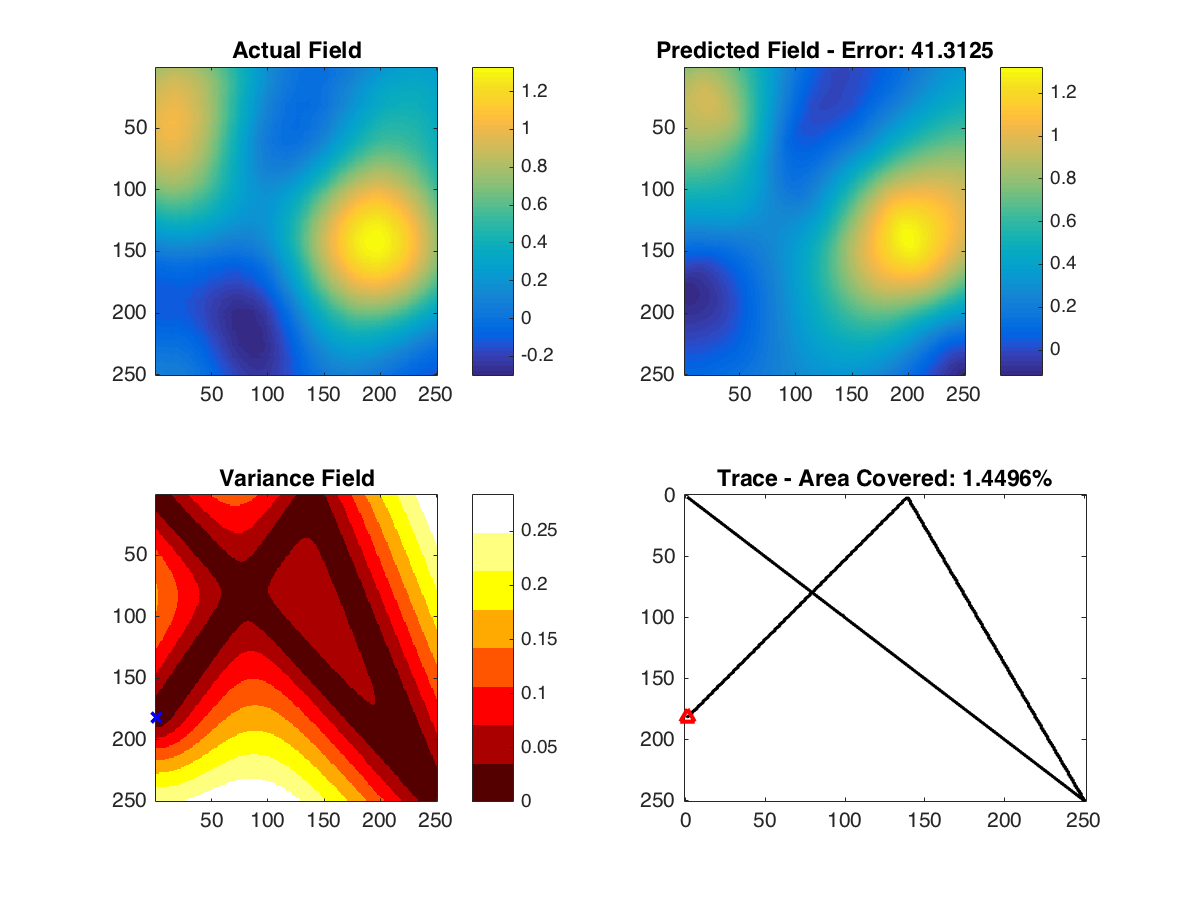
\includegraphics[width=0.95\linewidth]{figures/nhv_4panel.png}
    \captionsetup{skip=0.20\baselineskip,size=footnotesize}
	\caption{The Next Highest Variance (NHV) algorithm (Section \ref{sec:nvh_pp_alg} terminated after two iterations of the algorithm. The actual field that is being explored is shown in the upper left. The current prediction of the actual field is shown in the upper right. The variance of the current prediction of the field is shown in the lower left. The trace of the exploration vehicle's path taken to the point of termination (in red) is shown in the lower right panel. All distance units are in meters.}
	\label{fig:nhv_pp}
\end{figure}

\subsection{Inefficiency in NHV}
The NHV algorithm does not account for repeating paths, or avoiding re-sampling points. The only knowledge used is a single criteria of variance. Although the ground covered by the algorithm may be sufficient for the most exploration cases, a path planner that considers the cost of trajectories would likely yield better results.

\section{Monte Carlo Based Trajectory Finding}
A path planner designed for autonomous field exploration using a Monte Carlo path selection technique will be introduced. By first selecting a set of locations with the highest uncertainty in current prediction, the path planner will find a suitable path that will in turn minimize the average variance of the target field predictions. The problem can be stated as a sensor placement problem, where a suitable placement of sensors is found via a Monte Carlo simulation of the environment, and a minimization of the Kriging prediction variances \cite{kriging:sensorplacement}. Using Monte Carlo for trajectory finding for obstacle avoidance has been attempted \cite{janson:mcmp}, but not for exploration purposes.

In the case of the path planner, because the exploration vehicle is dynamic, the sensors can be thought of as being placed along the trajectory of the vehicle (assuming reasonable ergodicity of the target field). The Monte Carlo approach to path finding via the Kriging Method introduced will first find the points of highest prediction uncertainty on the target field, and then generate a finite set of random trajectories along the originally found trajectories. The trajectory that is predicted to reduce overall field uncertainty will be chosen as the path the vehicle will take.

\subsection{Finding Monte Carlo Trajectory Sets} \label{sec:mctrajsets}
After a suitable set of destinations are selected from the set of points containing the $N^{th}$ coordinates of highest uncertainty, $S_{v}$, trajectories to each point are calculated. The trajectories calculated can be both deterministic or variably non-deterministic walks from the current location of the exploration vehicle, to the final location.

For a given destination, $\vect{s}_d$ in $S_{v}$, and the current location of the vehicle, $\vect{s}_{c}$, a set of waypoints that establish the route between the start and finish points can be defined as $T_k = \Big\{[x_{k_1}\ y_{k_1}\ \theta_{k_1}]^T,\ [x_{k_2}\ y_{k_2}\ \theta_{k_2}]^T, \dots [x_{k_{i_f}}\ y_{k_{i_f}}\ \theta_{k_{i_f}}]^T \Big\}$, $i_f = \Big\lceil \frac{\|\vect{s}_c - \vect{s}_d\|_2}{\alpha} \Big\rceil$, where, $\alpha \in \mathbb{R}^{+}$, is a scaling variable representing the step size between waypoints, $x$ and $y$ are field coordinates, and $\theta$ is the heading angle of the vehicle. 

\begin{equation}
	T_{k_{i + 1}} = T_{k_i} +
	\begin{bmatrix}
		\alpha \cos \theta_{k_i} \\
		\alpha \sin \theta_{k_i} \\
		\text{atan2}(s_{d_y} - T_{k_{{i+1}_y}}, s_{d_x} - T_{k_{{i+1}_x}}))
	\end{bmatrix} + \begin{bmatrix} 
		\vect{w}_{k_{i+1}} \\
		0
	\end{bmatrix}
\end{equation}

Where $\vect{w}_k \in \mathbb{R}^2$ is a zero-mean Wiener Process with a tunable variance. Multiple Brownian walks from the current position to a given destination can be calculated to increase the pool of possible paths. For a zero variance Wiener process ($\text{var}\{\vect{w}\}=0$), the walk defined is deterministic, and equal to finding a set of N-NHV trajectories (Section \ref{sec:nnhv}. The \textit{cord} of the walk is the line the connects the initial position to the destination position. The cord acts as the expected value in the distribution of trajectories calculated. The initial point, $T_{k_1}$, and the final point, $T_{k_f}$, are defined explicitly.

\begin{equation}
	T_{k_1} = \begin{bmatrix}
		s_{c_x} \\
		s_{c_y} \\
		\text{arctan2}(s_{d_y} - s_{c_y}, s_{d_x} - s_{c_x})
	\end{bmatrix},\ 
	T_{k_f} = \begin{bmatrix}
		s_{d_x} \\
		s_{d_y} \\
		\theta_{f-1}
	\end{bmatrix}
\end{equation}

\begin{figure}[h!]
	\centering
	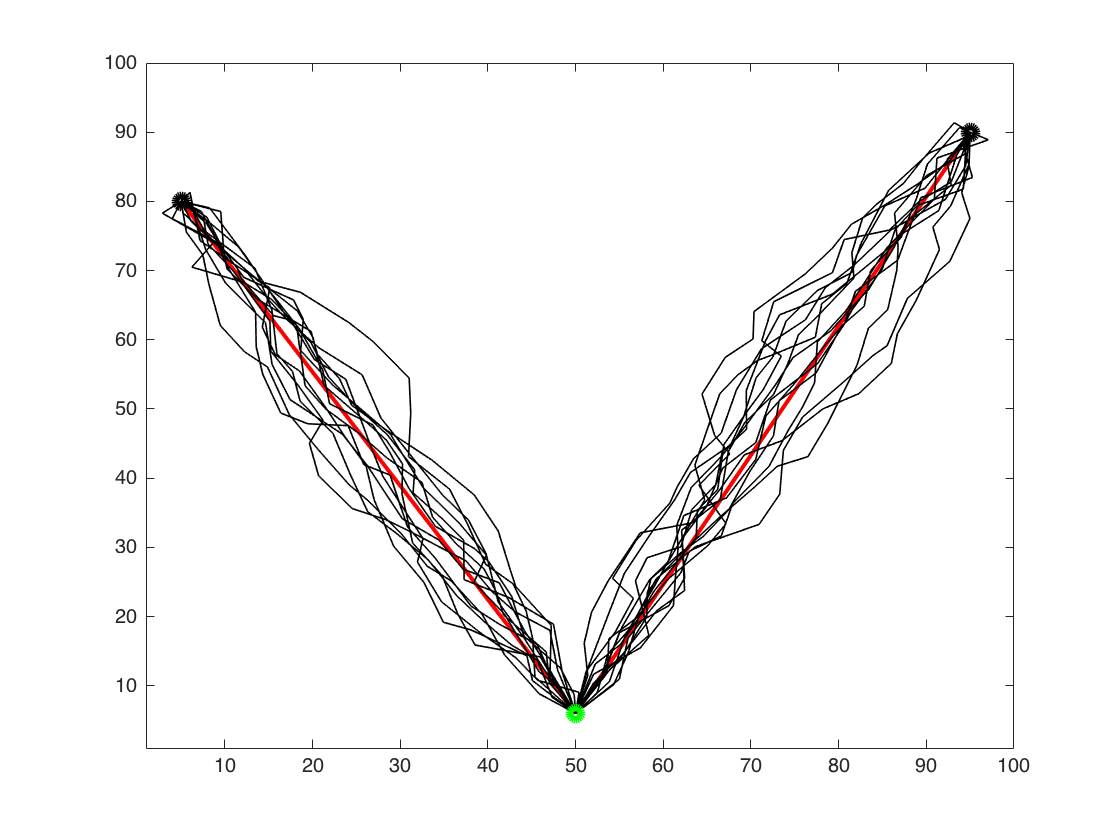
\includegraphics[width=0.8\linewidth]{figures/brownian_motion_mc.png}
	\caption{Brownian non-deterministic walks (black) surrounding deterministic cords (red). The starting point is indicated in green. For a set of $N=2$ possible trajectories, $15$ random walks around each trajectory with a variance of $10$. All distance units in meters.}
\end{figure}

\subsection{Selecting An Optimal Monte Carlo Trajectory} \label{sec:mcselbesttraj}
In Section \ref{sec:mctrajsets}, a set of possible trajectories, $T$ was defined. The trajectory that is ultimately chosen by the introduced path finder is the path that minimizes the average uncertainty of the predicted target field, i.e. maximizes the loss function, $L(T)$.
Let $\hat{Z}(S)$ be a Kriging predicted field from a set of samples at known locations. Furthermore, let $\hat{Z}(S+\hat{T}_k)$ be the a Kriging predicted field from the set $S$ concatenated with a virtual set of samples $\hat{T}_k$. The values in the set $\hat{T}_k$ have not necessarily been sampled, but they contain, as samples, the previously predicted values, $\hat{Z}(T_k)$, at the known locations in $T_k$.

\begin{equation}
	samples(\hat{T}_k) = \hat{Z}(T_k)
\end{equation}

The variance of the field with real and virtual samples, $\text{var}\{\hat{Z}(S+\hat{T}_k)\}$, can then be calculated. Using the definition for $\Sigma_{\text{var}}(\cdot)$ from Section \ref{eq:fielduncert}, the path chosen is the trajectory that satisfies:

\begin{equation}
	\label{eq:mcfoundpath}
	P = \argmin_{T_k}\ \Sigma_{\text{var}}(\text{var}\{\hat{Z}(S+\hat{T}_k)\})
\end{equation}

\subsection{Monte Carlo Path Planning Algorithm}
The exploration algorithm initializes by directing the vehicle to sweep across the forward diagonal of the target field to collect an initial set of samples. An initial variogram is fit, and a Kriging prediction of the field is then made. The variances of all points on the target field are then calculated. The set, $S_{v}$, of points with the $N$ highest prediction variances are found (Section \ref{sec:highestvars}). A set of trajectories, $T$, is then calculated (Section \ref{sec:mctrajsets}). The trajectory that is predicted to minimize the total uncertainty of the target field is chosen as the next path of the exploration vehicle (Section \ref{sec:mcselbesttraj}). Once the vehicle completes the last path chosen, the field values and variances are predicted and calculated again. A new path is chosen in the same fashion. The algorithm terminates when it can no longer choose a path that can be accomplished with the amount of fuel that remains within the exploration vehicle. Another case of planner termination occurs When the average prediction variance of the field is zero, which ideally occurs when all locations have been sampled.

An algorithm for Kriging Monte Carlo Path Planning (Kriging MCPP) for a target field, $Z$, of size ($h\times w$) is introduced in Algorithm \ref{alg:mcpp}. The initial location of the vehicle is set to $\vect{s}_{c} = [0\ 0]^T$. The vehicle starts the path planner with $F$ units of fuel.

\begin{algorithm}[h!]
\caption{Monte Carlo Path Planning (MCPP) with The Kriging Method}\label{alg:mcpp}
\begin{algorithmic}[1]
\Procedure{Kriging\_MCPP}{$Z$}
	\BState \emph{Conduct Initial Sweep}:
	\State SetWaypoint($[h\ w]^T$)
	\BState \emph{Krig The Field}:
	\State $\hat{Z}, \text{var}\{\hat{Z}\}$ = KrigingPredictField($Z$, $S$)

	\BState \textbf{while} $F > 0$ \textbf{and} $\Sigma_{\text{var}} > 0$:
	\State $P = []$
	\State $\Sigma_{\text{min}} = \infty$ \\

	\BState \ \ \ \ \emph{Find the highest field variances}:
	\State \ \ \ \ \textbf{for}\ $k = 1 \text{:} N$
	\State \ \ \ \  \ \ \ \ $S_{v}(k) = \argmax_{\vect{s}} \ \text{var}\{\hat{Z}_{k}(\vect{s})\}$
	\State \ \ \ \ \ \ \ \ $\text{var}\{\hat{Z}_{k+1}(\vect{s})\} = \text{var}\{\hat{Z}_{k}(\vect{s})\} - S_{v}(k)$\\

	\BState \ \ \ \  \emph{Calculate trajectories to all points found}:
	\State \ \ \ \  $\forall s_k \in S_{v}(k)$:
	\State \ \ \ \  \ \ \ \ $s_d = s_k$
	\State \ \ \ \  \ \ \ \ $f = \Big\lceil \frac{\|\vect{s}_c - \vect{s}_d\|_2}{\alpha} \Big\rceil$
	\State \ \ \ \  \ \ \ \ $T(1) = \begin{bmatrix} s_{c_x} \\ s_{c_y} \\ \text{arctan2}(s_{d_y} - s_{c_y}, s_{d_x} - s_{c_x}) \end{bmatrix}$
	\State \ \ \ \  \ \ \ \ $\forall i \in (1, f - 1)$:
	\State \ \ \ \  \ \ \ \  \ \ \ \ $T(i+1) = T(i) + \begin{bmatrix} \alpha \cos \theta(i) \\ \alpha \sin \theta(i) \\ \text{atan2}(s_{d_y} - T(i)_y, s_{d_x} - T(i)_x) \end{bmatrix} + \begin{bmatrix} \vect{w}(i) \\ 0 \end{bmatrix}$
	\State \ \ \ \  \ \ \ \ $T(f) = \begin{bmatrix} s_{d_x} \\ s_{d_y} \\ \theta_{f-1} \end{bmatrix}$\\

	\BState \ \ \ \  \ \ \ \  \emph{Calculate estimated field confidence for trajectory computed}:
	\State \ \ \ \  \ \ \ \  $\forall i \in [1, f]$:
	\State \ \ \ \  \ \ \ \  \ \ \ \ $\text{samples}(\hat{S}_T)$ += $\hat{Z}(T(i))$
	\State \ \ \ \  \ \ \ \  \ \ \ \ $\text{locations}(\hat{S}_T)$ += $T(i)$
	\State \ \ \ \  \ \ \ \  \ \ \ \ $\hat{Z}_T, \text{var}\{\hat{Z}\}_T$ = KrigingPredictField($Z$, $\hat{S}_T$)
	\State \ \ \ \  \ \ \ \  \ \ \ \ $\Sigma_{\text{var}}(T) = \text{avg}(\text{var}\{\hat{Z}\}_T)$\\

	\State \ \ \ \  \ \ \ \  \ \ \ \ \textbf{if} $\Sigma_{\text{var}}(T) < \Sigma_{\text{min}}$ \textbf{and} \text{length($T$)} $< F$:
	\State \ \ \ \  \ \ \ \  \ \ \ \ \ \ \ \ $\Sigma_{\text{min}} = \Sigma_{\text{var}}(T)$
	\State \ \ \ \  \ \ \ \  \ \ \ \ \ \ \ \ $P = T$\\

	\BState \ \ \ \  \emph{Navigate through the chosen path}:
	\State \ \ \ \  $\forall p \in P$:
	\State \ \ \ \  \ \ \ \ SetWaypoint($p$) 
\EndProcedure
\end{algorithmic}
\end{algorithm}

In Algorithm \ref{alg:mcpp}, the function \texttt{SetWaypoint()} is an abstracted function which steers the vehicle in the direction of the waypoint specified, and blocks the code instruction until the waypoint has been met. The function \texttt{length(}$T$\texttt{)} finds the arc length of the path by connecting all points in the trajectory, $T$. For a deterministically calculated trajectory, $T$, the arc length is $\alpha |T|$.

\begin{figure}[hb!]
	\centering
	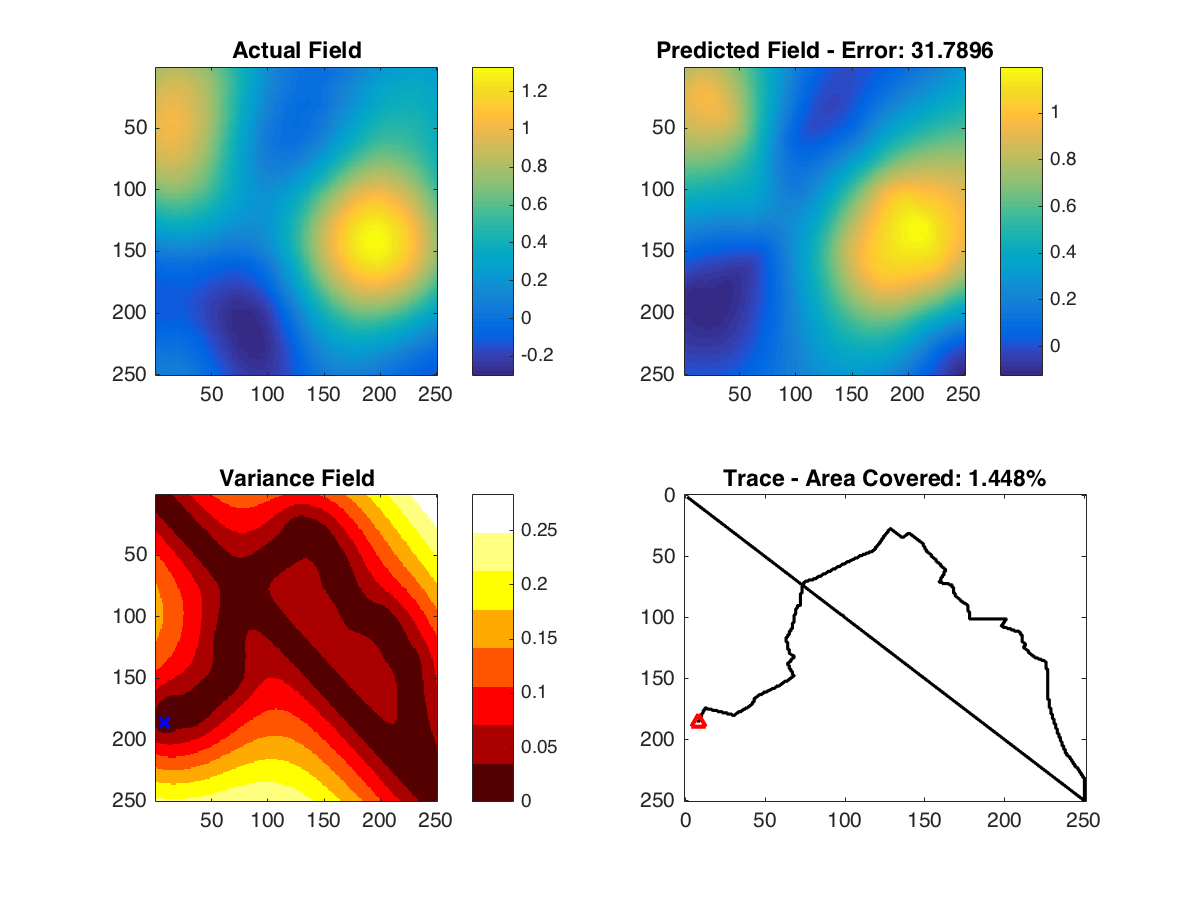
\includegraphics[width=0.95\linewidth]{figures/mc_4panel.png}
    \captionsetup{skip=0.20\baselineskip,size=footnotesize}
	\caption{The Next Highest Variance (NHV) algorithm (Section \ref{sec:nvh_pp_alg} terminated after two iterations of the algorithm. The actual field that is being explored is shown in the upper left. The current prediction of the actual field is shown in the upper right. The variance of the current prediction of the field is shown in the lower left. The trace of the exploration vehicle's path taken to the point of termination (in red) is shown in the lower right panel. All distance units are in meters. Here, $N$, the number of endpoints selected is $3$, and the number of random paths per cord calculated is $15$.}
	\label{fig:mcpp}
\end{figure}

\subsection{$N$ Next Highest Variances Algorithm (Zero Variance MCPP)} \label{sec:nnhv}
A small modification to the NHV algorithm can be made to consider more trajectories. If the set of highest variances on the field, $S_v$ has a cardinality greater than $1$ ($N > 1$), $N$ trajectories can be made, and weighed against each other in terms of their return on investment (as discussed in Section \ref{sec:mctrajsets}). This is done by selecting a zero variance gain on the noise of each Monte Carlo Path, and only calculating a single cord per endpoint. By weighing $N$ Next Highest Variances (N-NHV) against one another, more methodical routes can be taken. It may not always be the case that simply exploring the next highest variance will yield a smaller field variance. If a smaller prediction variance location is selected as the endpoint location (i.e. an endpoint that is not necessarily the first coordinate in the set $S_v$), the vehicle might sample more unknown points along the way, versus potentially rescanning already sampled area with the simple NHV algorithm.

\subsection{Benefits in MCPP over NHV}
The Monte Carlo based path planner takes into account a set of trajectories, and compares their estimated return on investment. The NHV simply takes the path to the high prediction uncertainty location. Though the MCPP algorithm, with a non-zero noise variance, does not deterministically calculate its trajectories, given enough trajectories, the algorithm could find a path that will reduce overall field uncertainty in a more methodical way over the NHV algorithm.

\subsection{Disadvantages of The Monte Carlo Path Planner}
The MCPP algorithm does not calculate the cost of each next move taken, but rather a set of waypoints taken. In other words, the algorithm only takes into account entire trajectories at a time. A more optimal approach to this planner would be to take into consideration the cost of each waypoint selected. A remedy to this problem using the MCPP would be to increase the number of random trajectories calculated for each cord.


\part{Simulation \& Results}
\chapter{Simulation Framework}
Using \textit{MATLAB}, the method described in Algorithm \ref{alg:uncert} was implemented to provide a simulation environment to show the effectiveness of such a method. The target field in the simulation is a variable sized field with a single state of interest. The autocorrelation factor of the field in the simulation is an adjustable variable that determines the likeliness of each pair of neighboring points as a function of distance. 

The simulation includes a software in the loop vehicle with variable dynamics and incorporates the ability to follow a preplanned route. The simulation will be used to demonstrate the abilities of the algorithm described, and comparisons to an algorithm with a preplanned trajectory. 

\section{Simulated UAV Model Dynamics}
The vehicle dynamics of the UAV in the simulation are modeled off of a Dubins' Vehicle. Assume a two dimensional field where the axes are labeled $x_1$ and $x_2$ respectively. The simulated UAV has constant vehicle velocity of $v$, and a heading angle, $\theta$ with a turning rate of $u$, where the turning radius is fixed. The kinematics of such a system is defined to be:

\begin{equation}
	\begin{bmatrix}
		\dot{x_1} \\
		\dot{x_2} \\
		\dot{\theta} \\
	\end{bmatrix} = 
	\begin{bmatrix}
		v \cos \theta \\
		v \sin \theta \\
		u
	\end{bmatrix}
\end{equation}

\section{Generating a Target Field}
The simulation yields a target field that is of variable size. Each vesicle in the field is exactly the area of the sensor footprint of the simulated UAV. This is to make the sensor measurements as ideal as possible, so no samples are missed when a vesicle is flown over.

The field is composed of a single feature which is geospatially autocorrelated. Initially, the points on the field are generated from a normal distribution with a standard deviation of $1$, and expected value of $0$. The field is then convolved with a two dimensional Gaussian filter with a variable standard deviation, $\sigma_{\text{field}}$. The final filter ``smooths" the field in order to simulate autocorrelation. The result is a randomly-generated, variably-sized, and autocorrelated field with a unit-less feature of interest.

\section{Caveats of Simulation}
Though the addition of these kinematics make the simulation more representative of real life aircraft dynamics, the UAV simulated will be mimicking the dynamics of a multi-rotor with a very small radius of turn (ROT) ($r < 0.1 [\text{m}]$). The simulation with this aircraft is not concerned with velocity because a sample is taken at every possible position the aircraft hovers above. Furthermore, the target field in the simulation is fully-ergodic, and the speed of flight does not change the quality of prediction.

\section{Examples of Use}

\chapter{Results}
The three path planners (NHV, N-NHV, and MCPP) introduced in Chapter \ref{ch:pp} all aim to reduce the overall prediction uncertainty of a field given a limited amount of flight time. They accomplish the task by calculating variances of a target field's predictions and attempting to choose a trajectory that reduces overall uncertainty. 

\section{Comparing The Method}
A common approach to exploration and patrolling problems is the use of a spiral, zig-zag, or lawn mower pattern. The methods introduced will be compared to equally time limited version of a zig-zagging approaches seen in Nikhil Nigam, et al. Control and Design of Multiple Unmanned Air Vehicles for a Persistent Surveillance Task (Part II.C.3, Figure 6, \cite{nigam:zigzag}). The method, for the sake of fairer comparison, will run a Kriging prediction and variance calculation on the samples taken using the zig-zag explorer. This is to generate measurable and comparable metrics against the path planners introduced. The path planners introduced will be compared against the zig-zag exploration method shown in Figure \ref{fig:zigzag4}.

\begin{figure}[hbt!]
    \centering
    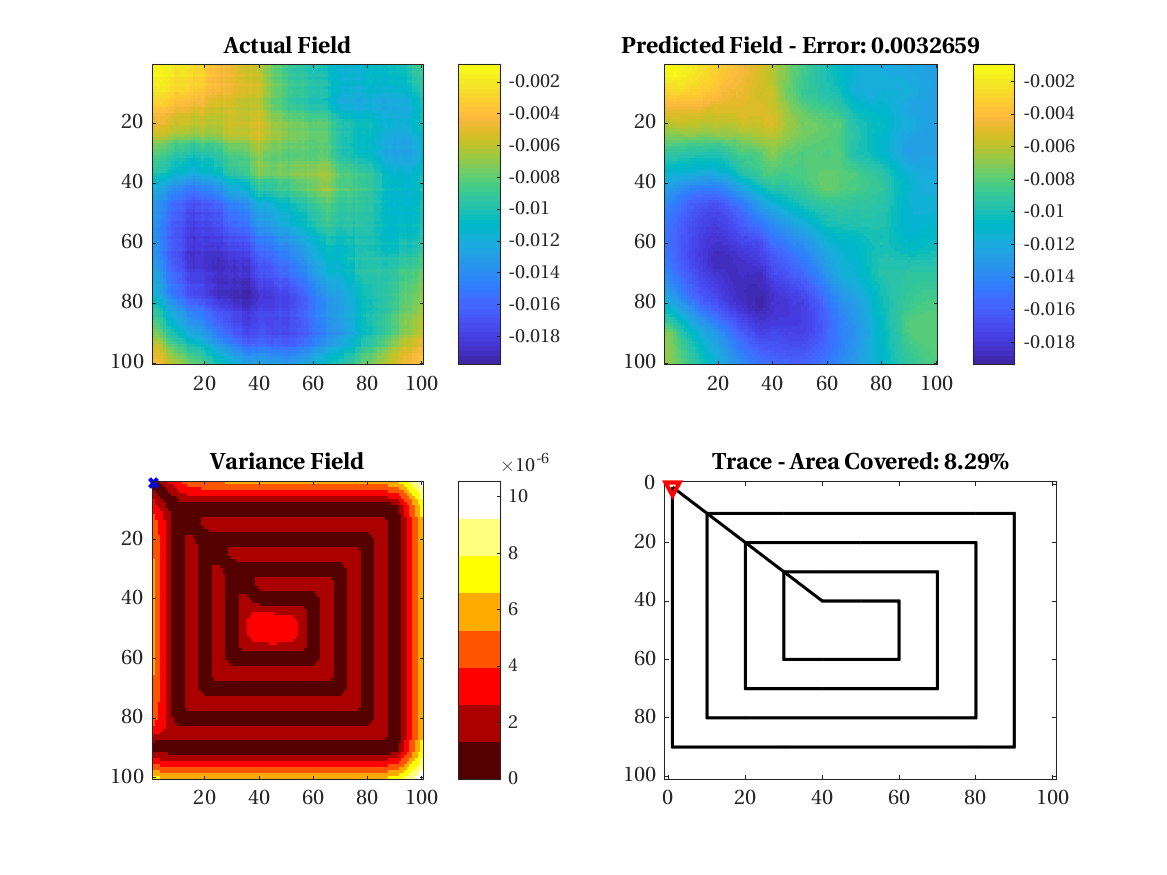
\includegraphics[width=0.9\linewidth]{figures/hbresults/zz_10p_100x100_sf_25_seed_2.png}
    \captionsetup{skip=0.20\baselineskip,size=footnotesize}
    \caption{Zig-Zag exploration method set to scan a fixed percentage of a target field. A Kriging prediction and variance calculation is computed after completing the maneuver. The actual field that is being explored is shown in the upper left. The current prediction of the actual field is shown in the upper right. The variance of the current prediction of the field is shown in the lower left. The trace of the exploration vehicle's path taken to the point of termination (in red) is shown in the lower right panel. All distance units are in meters.}
    \label{fig:zigzag4}
\end{figure}

\subsection{Variance Drop Calculation}
The variance of every target field over each iteration will be the average prediction variance of the field after every prediction recalculation. This criteria is introduced in Section \ref{sec:fielduncert} on field uncertainty. This metric relates prediction quality of the path planner to its predicted prediction quality. A drop in variance over iterations should signal a better prediction of the target field over that iteration, and less overall uncertainty of the target field.

\subsection{Simulation Results}
% The effectiveness of the method introduced varies based on the area of the target field being explored. For small fields, a naive zig-zag exploration may be more efficient and less computationally expensive. By modulating the dimensions of the target field, a comparison can be drawn demonstrating the effectiveness of the method versus a naive zig-zag approach.
The methods introduced will be compared to one another and the zig-zag method for the same termination condition. Each method will stop the field exploration process when the exploration vehicle traverses a fixed path length expressed in terms of the area percentage scanned, $A_{scan}$. For example, if the maximum scan percentage of a size $w \times h$ size field is $p\%$, then the method will stop exploring when $A_{scan} = \frac{p}{100}wh$ number of vesicles have been sampled. In an effort to allow the zig-zag method to cover as much of the field as possible, the spacing between each spiral bound, $r$, will be pre-calculated.

\begin{equation}
    r = \frac{100}{p}
\end{equation}

\subsection{Simulation Result Parameters}
The number of trajectories compared in both the NNHV and MCPP methods is $N=5$. For the MCPP method, an additional $20$ Monte Carlo trajectories are calculated for each of the $N$ trajectories. The target field size of the fields compared in the simulation have unit-less vesicle dimensions of $100\times 100$. Two random number generator seeds ($2$, $3$) are used to generate two sets of runs in an effort to show the methods for a variety of random fields. The autocorrelation factors of the field will be varied in an effort to show the effectiveness of the methods for different field statistics. When the prediction variances of the methods are compared, the values are normalized to an a priori mean variance, which is equal to the mean variance of the field generated from running a Kriging prediction on the equivalent field from a set of samples taken from the first five forward diagonal vesicles on the target field.

\subsection{Prediction Error Calculation}
The quality of each path planner will be judged by its ability to explore a field in a fixed amount of time. The prediction error of each method will be used as a metric of path planning quality. The actual values of the fields scanned are known in simulation, and for each rerouting iteration, the predictions and prediction errors will be recalculated.

The prediction error function, erf$(Z,\hat{Z})$, will be the average root mean square (RMS) value for all $N$ field predictions made, point by point, on the actual field, $Z$, and the predicted field, $\hat{Z}$.

\begin{equation}
\text{erf}(Z, \hat{Z}) = \frac{1}{N}\sum_{\forall i \in Z} (Z(\vect{s}_i) - \hat{Z}(\vect{s}_i))^2
\end{equation}

\section{Comparing to Greedy Next-Best-View}
A course field of size $20 \times 20$ vesicles was generated with a autocorrelation factor, $\sigma_{field}$, equal to $4$, and limited to a $30\%$ scan.

\begin{figure}[htb!]
    \centering
    \begin{subfigure}[t]{0.3333\textwidth}
        \centering
        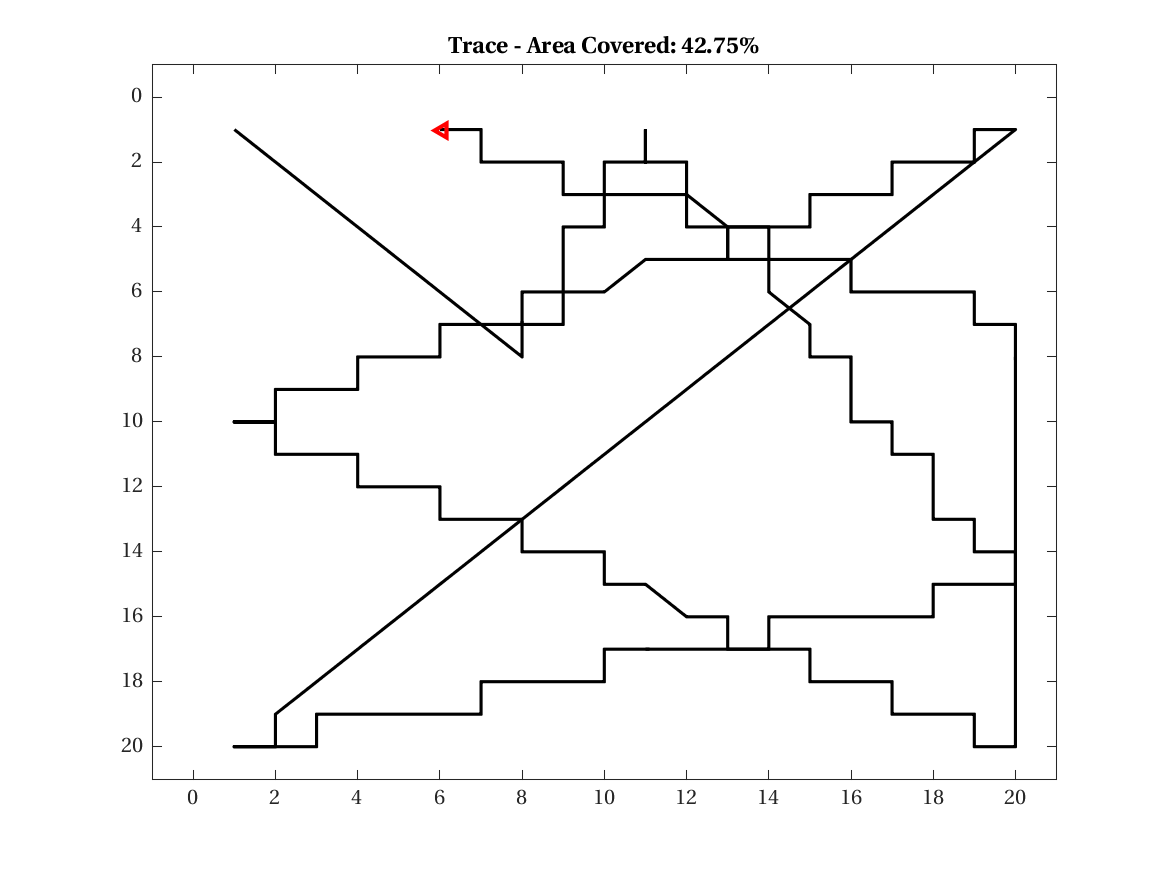
\includegraphics[width=\linewidth]{figures/hbresults/path_nhv_40p_20x20_sf_4_seed_2.png}
        \captionsetup{skip=0.20\baselineskip,size=footnotesize}
        \caption{Highest Variance}
    \end{subfigure}%
    \begin{subfigure}[t]{0.3333\textwidth}
        \centering
        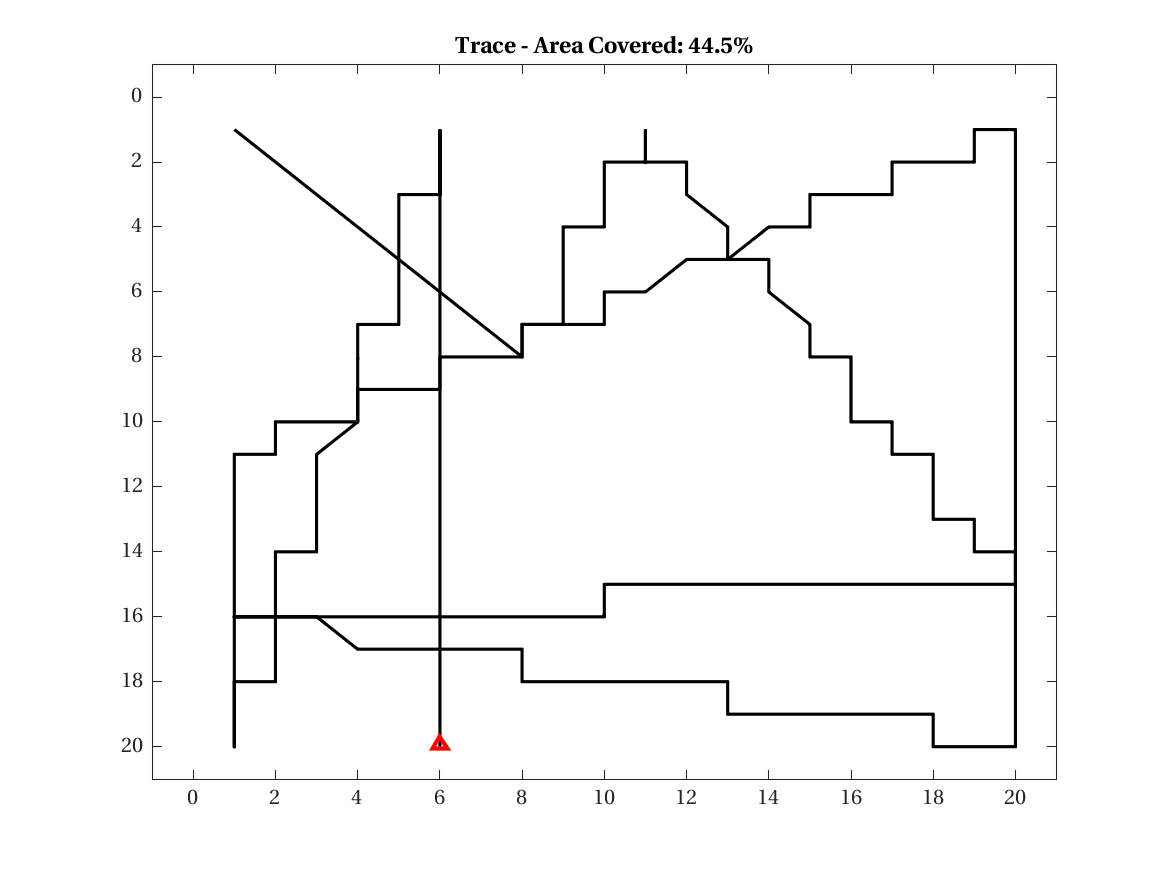
\includegraphics[width=\linewidth]{figures/hbresults/path_nnhv_40p_20x20_sf_4_seed_2.png}
        \captionsetup{skip=0.20\baselineskip,size=footnotesize}
        \caption{$N$ Highest Variance}
    \end{subfigure}%
    \begin{subfigure}[t]{0.3333\textwidth}
        \centering
        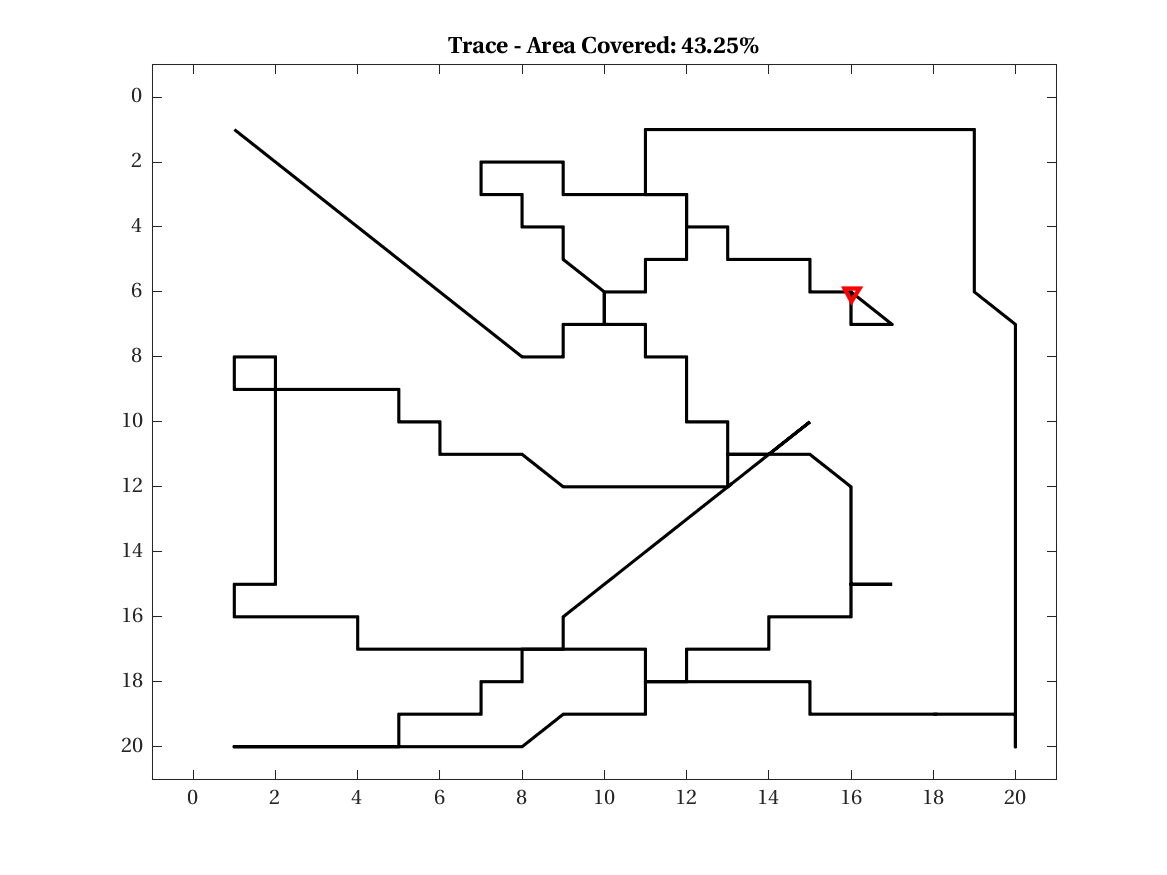
\includegraphics[width=\linewidth]{figures/hbresults/path_mc_40p_20x20_sf_4_seed_2.png}
        \captionsetup{skip=0.20\baselineskip,size=footnotesize}
        \caption{Monte Carlo}
    \end{subfigure}%
    \\
    \begin{subfigure}[t]{0.3333\textwidth}
        \centering
        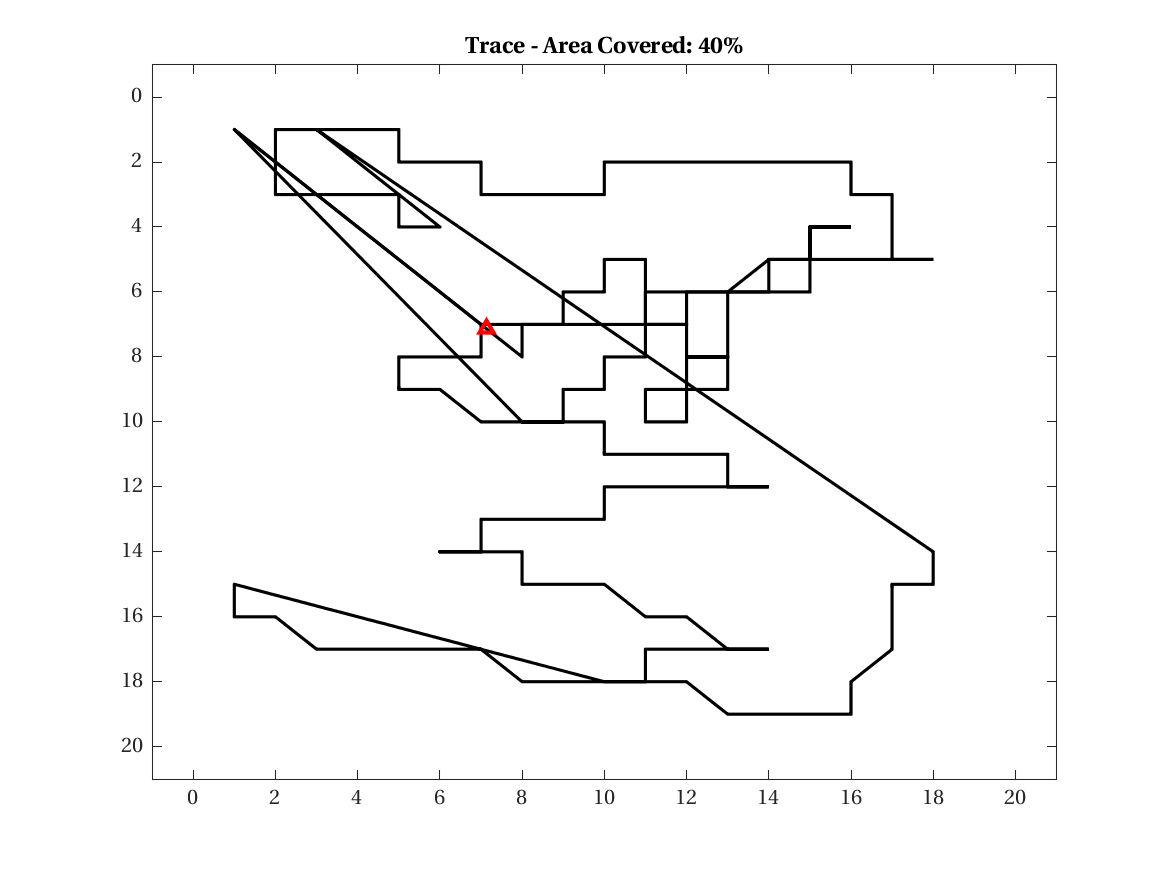
\includegraphics[width=\linewidth]{figures/hbresults/path_nbv_40p_20x20_sf_4_seed_2.png}
        \captionsetup{skip=0.20\baselineskip,size=footnotesize}
        \caption{Greedy NBV}
    \end{subfigure}%
    \begin{subfigure}[t]{0.3333\textwidth}
        \centering
        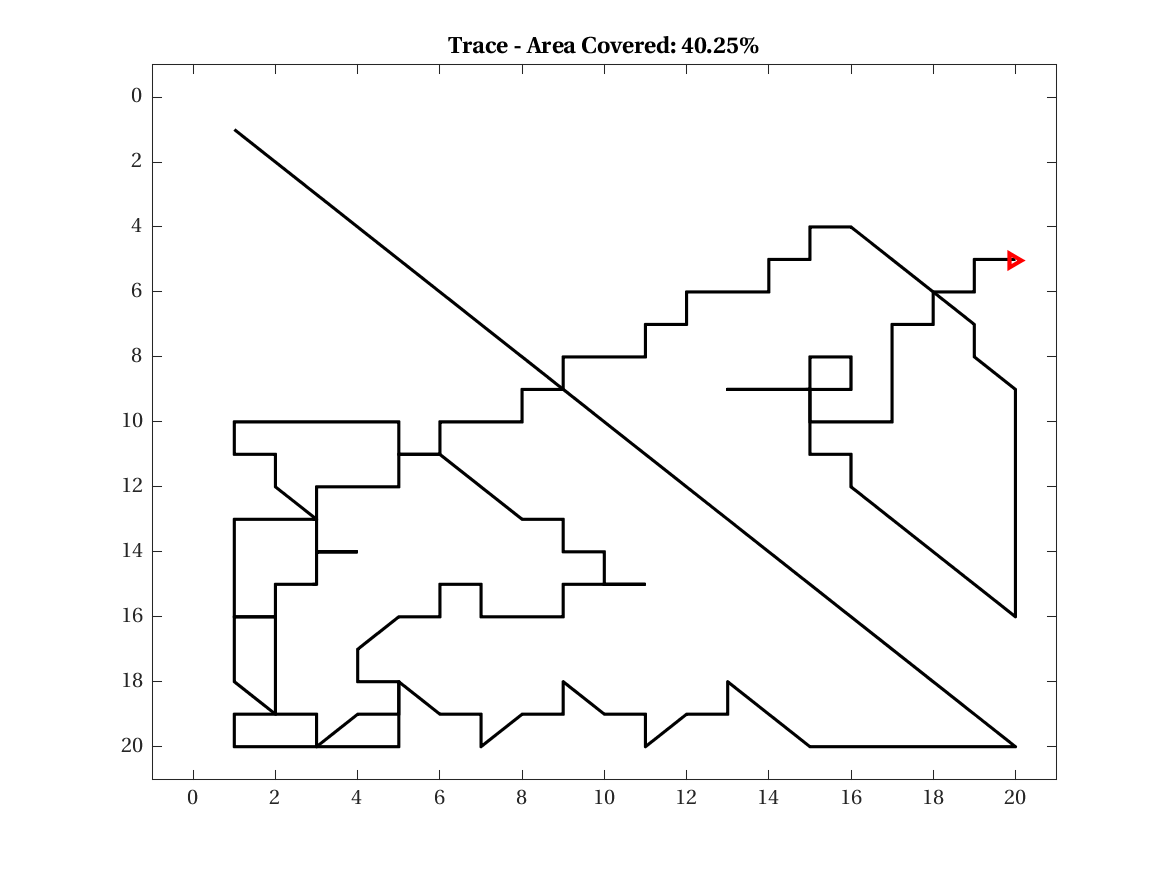
\includegraphics[width=\linewidth]{figures/hbresults/path_gradient_40p_20x20_sf_4_seed_2.png}
        \captionsetup{skip=0.20\baselineskip,size=footnotesize}
        \caption{Gradient Ascent}
    \end{subfigure}%
    \begin{subfigure}[t]{0.3333\textwidth}
        \centering
        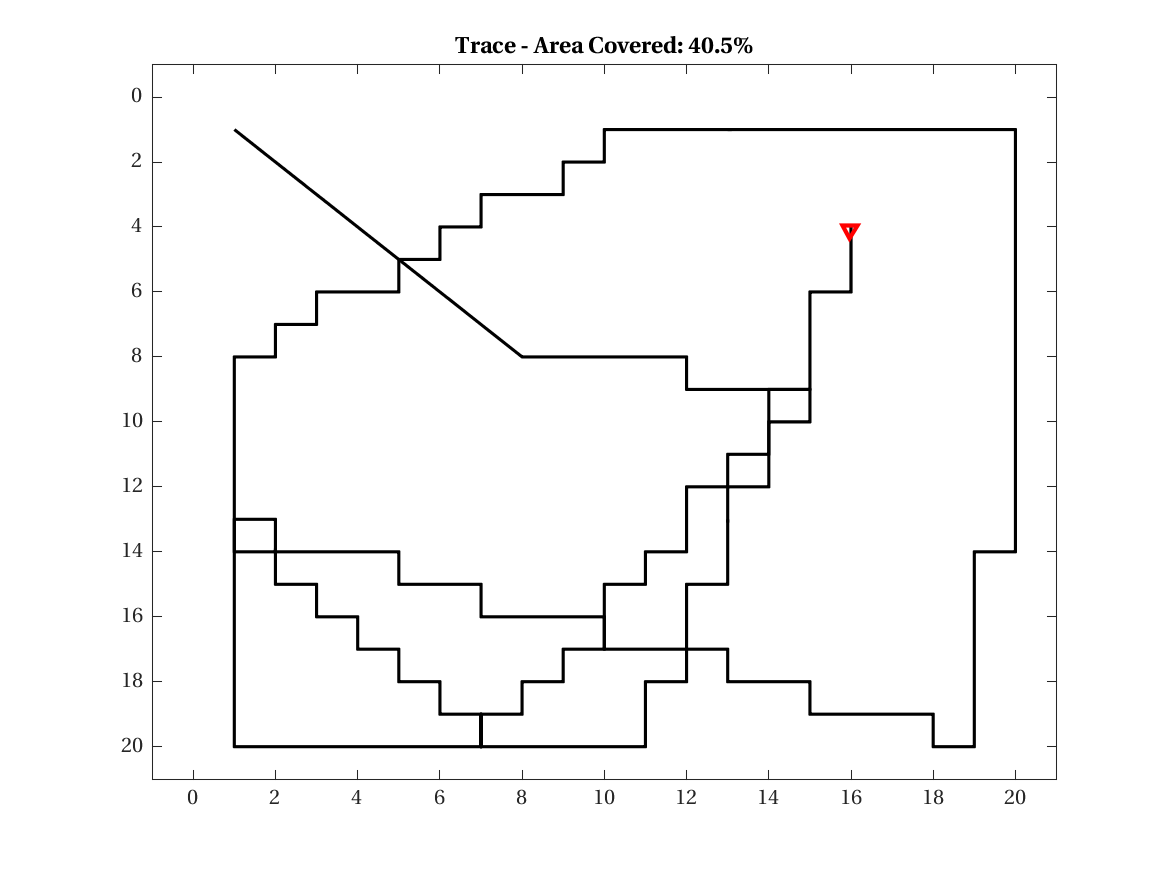
\includegraphics[width=\linewidth]{figures/hbresults/path_gr_40p_20x20_sf_4_seed_2.png}
        \captionsetup{skip=0.20\baselineskip,size=footnotesize}
        \caption{Gradient Range Ascent}
    \end{subfigure}%
    \\
    \begin{subfigure}[t]{0.3333\textwidth}
        \centering
        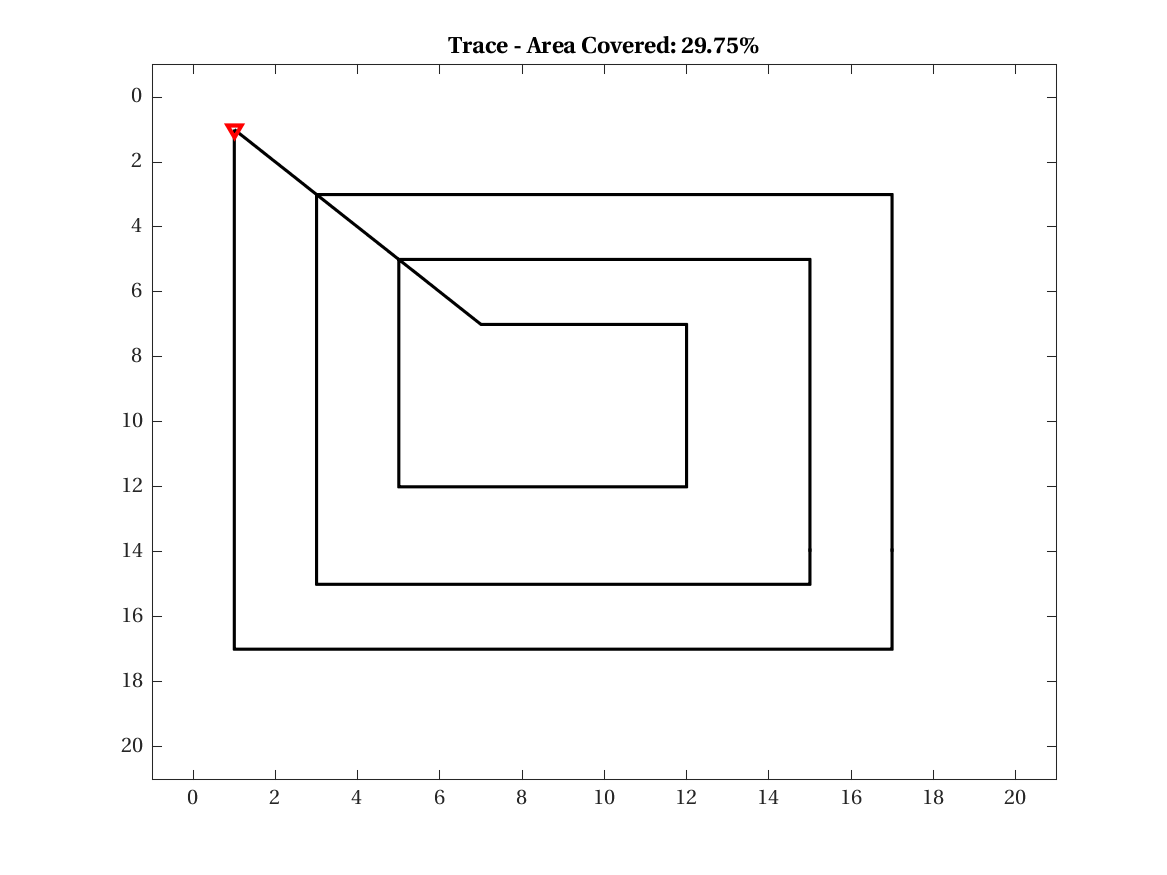
\includegraphics[width=\linewidth]{figures/hbresults/path_zz_40p_20x20_sf_4_seed_2.png}
        \captionsetup{skip=0.20\baselineskip,size=footnotesize}
        \caption{$ZZ_{30}$}
    \end{subfigure}%
    \captionsetup{skip=0.20\baselineskip}
    \caption{Exploration of a field of size $20 \times 20$, $\sigma_{field} = 4$, random seed 2.}
    \label{fig:nbvpathcomp}
\end{figure}

\begin{figure}[htb!]
    \centering
    \begin{subfigure}[t]{0.75\textwidth}
        \centering
        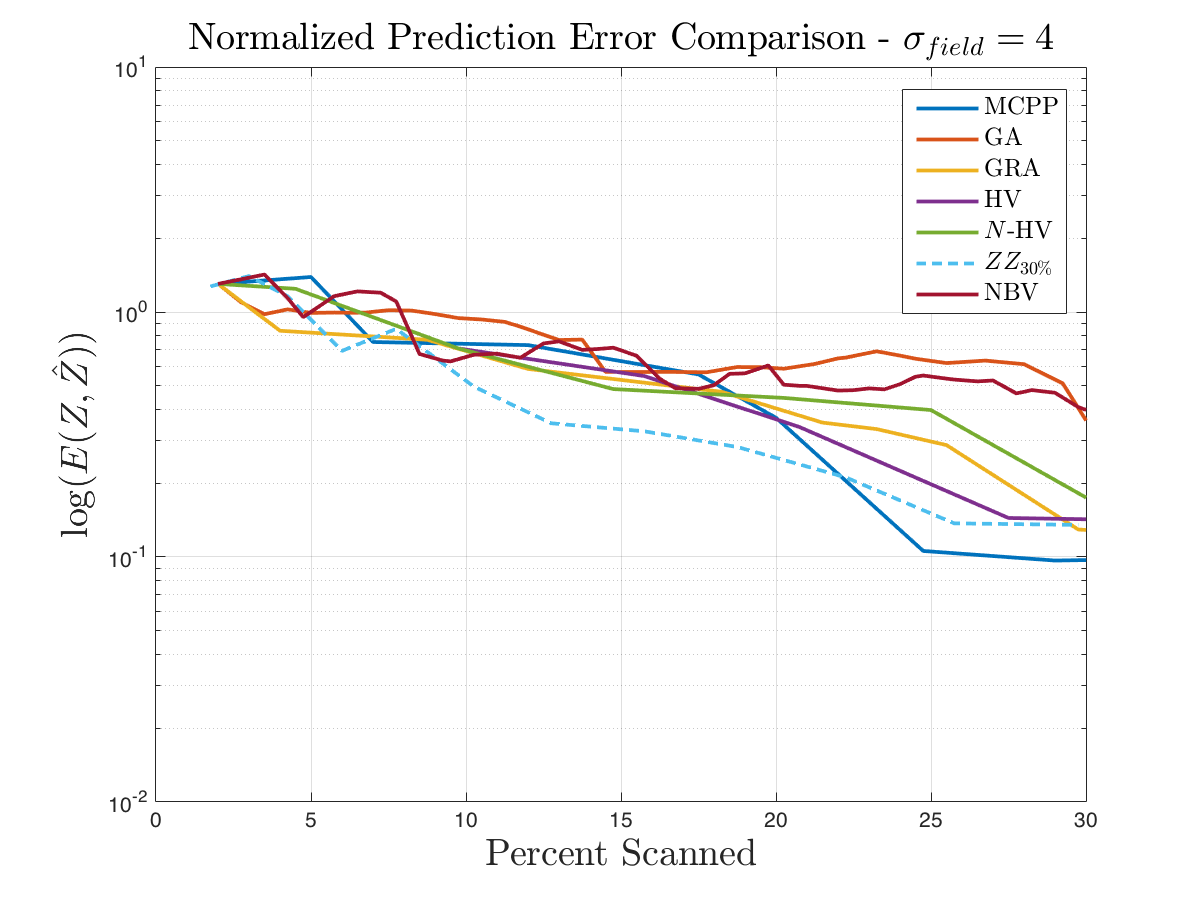
\includegraphics[width=\linewidth]{figures/results/normalized_errors_40p_20x20_sf_4_seed_2_app_10.png}
        \captionsetup{skip=0.20\baselineskip,size=footnotesize}
        \caption{Normalized prediction errors for each method.}
    \end{subfigure}%
    \\
    \begin{subfigure}[t]{0.75\textwidth}
        \centering
        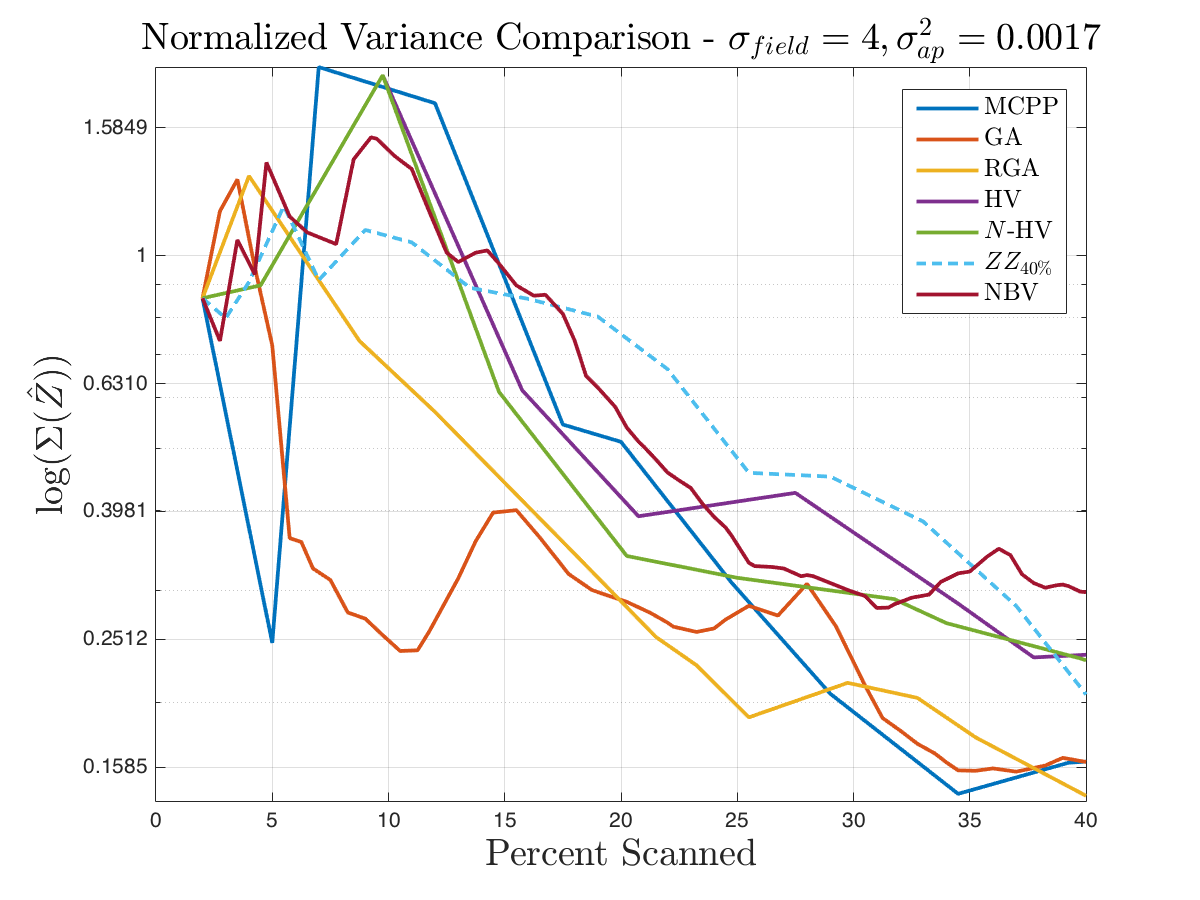
\includegraphics[width=\linewidth]{figures/results/normalized_variances_40p_20x20_sf_4_seed_2_app_10.png}
        \captionsetup{skip=0.20\baselineskip,size=footnotesize}
        \caption{Normalized prediction variances for each method.}
    \end{subfigure}%
    \captionsetup{skip=0.20\baselineskip}
    \caption{Prediction error and variances for an exploration of a field of size $20 \times 20$, $\sigma_{field} = 4$, random seed 2.}
    \label{fig:nbvcomp}
\end{figure}

\FloatBarrier
\clearpage

\section{High Spatial Autocorrelation Results}
The methods will be compared on target fields generated with an autocorrelation factor, $\sigma_{field}$, equal to the field width. A Gaussian filter $G(x,y,100)$ (Equation \ref{eq:gauss_filt}), is convolved with all points on the field.

\begin{figure}[htb!]
    \centering
    \begin{subfigure}[t]{0.3333\textwidth}
        \centering
        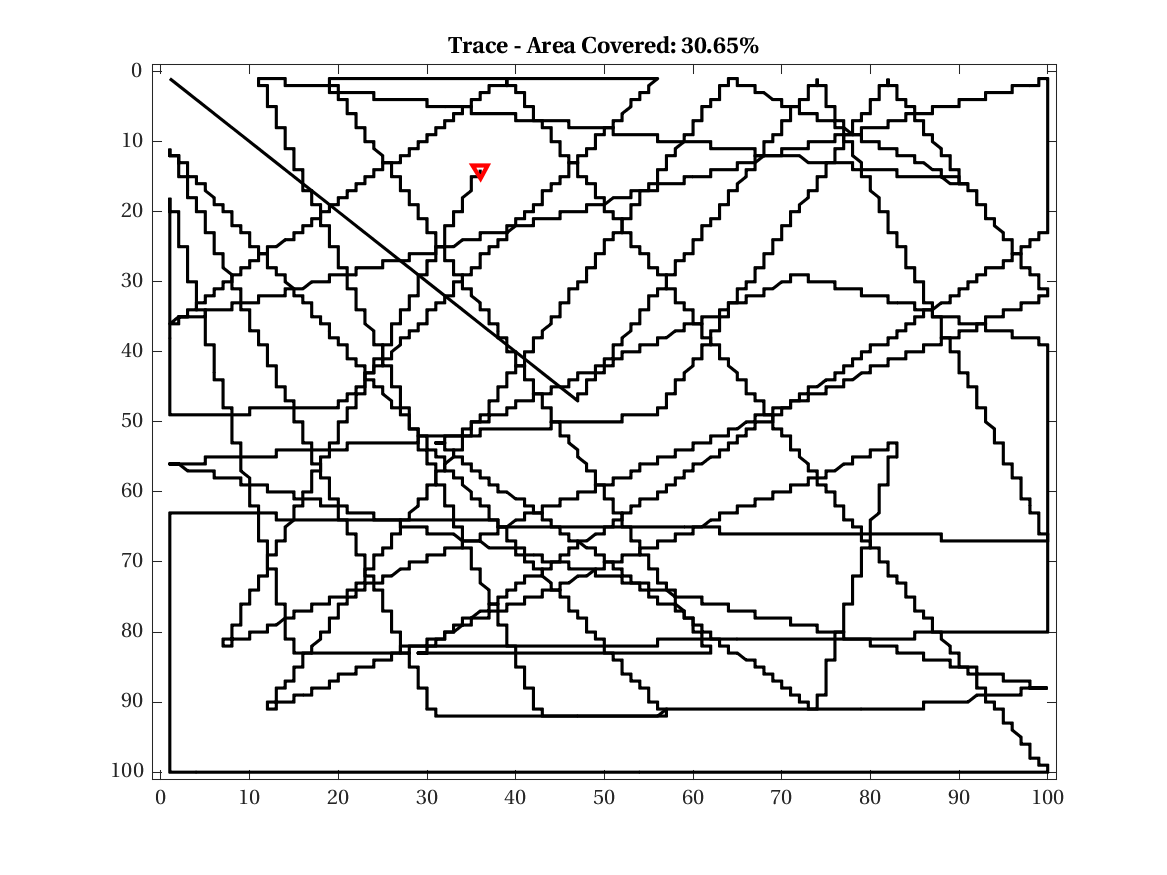
\includegraphics[width=\linewidth]{figures/hbresults/path_nhv_30p_100x100_sf_100_seed_2.png}
        \captionsetup{skip=0.20\baselineskip,size=footnotesize}
        \caption{Highest Variance}
    \end{subfigure}%
    \begin{subfigure}[t]{0.3333\textwidth}
        \centering
        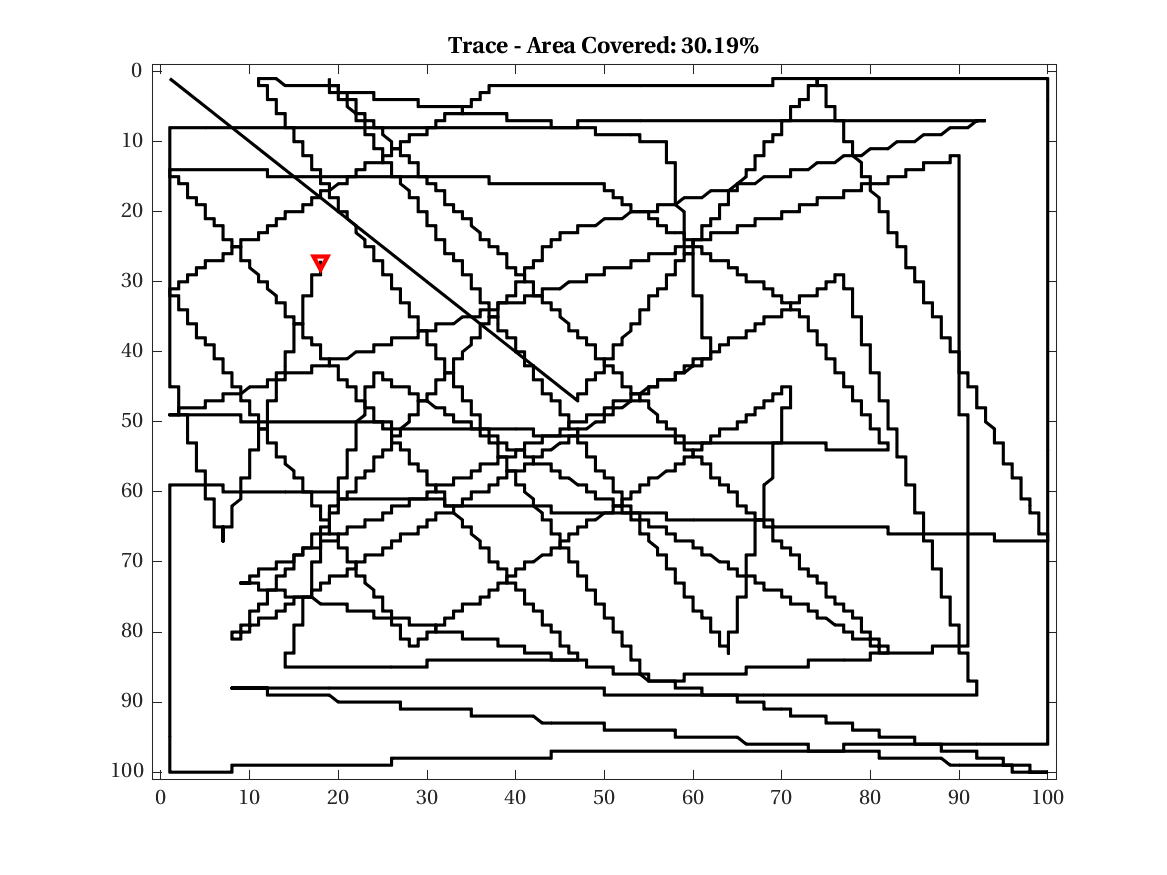
\includegraphics[width=\linewidth]{figures/hbresults/path_nnhv_30p_100x100_sf_100_seed_2.png}
        \captionsetup{skip=0.20\baselineskip,size=footnotesize}
        \caption{$N$ Highest Variance}
    \end{subfigure}%
    \begin{subfigure}[t]{0.3333\textwidth}
        \centering
        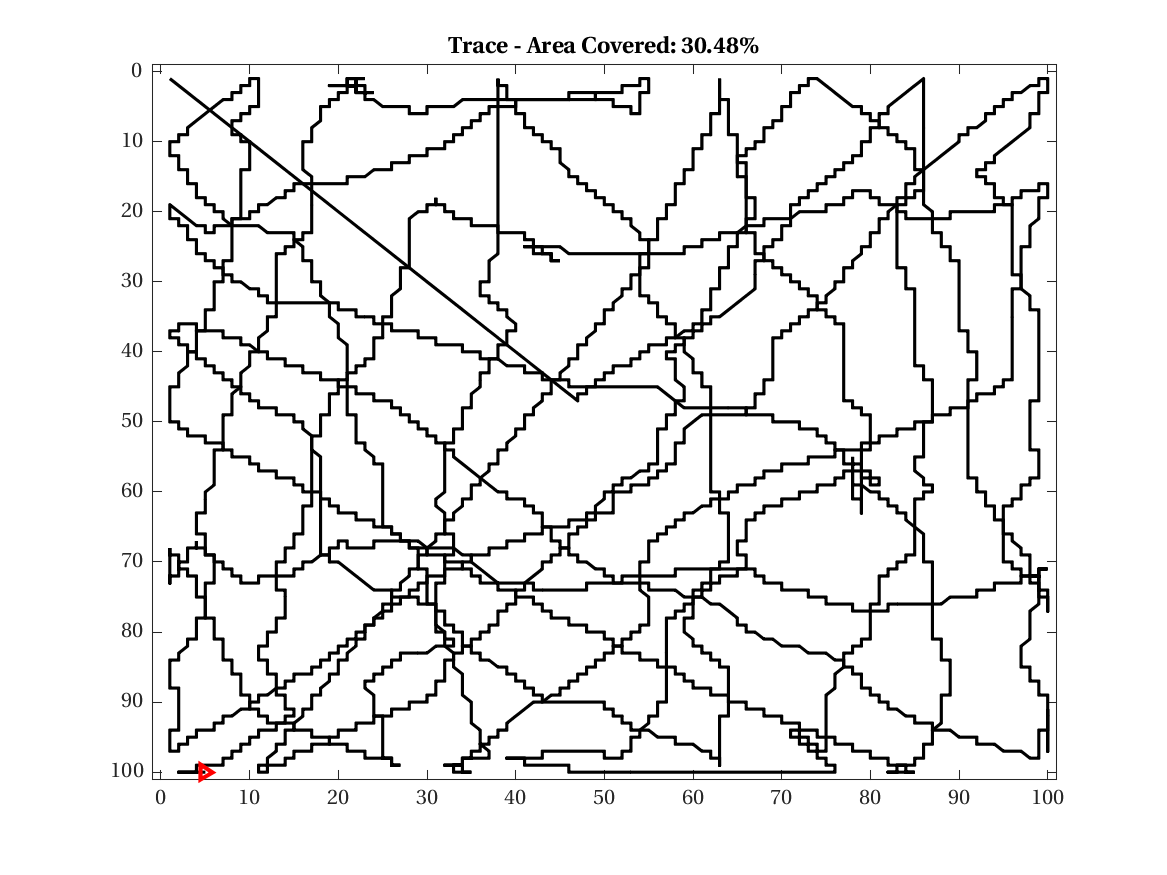
\includegraphics[width=\linewidth]{figures/hbresults/path_mc_30p_100x100_sf_100_seed_2.png}
        \captionsetup{skip=0.20\baselineskip,size=footnotesize}
        \caption{Monte Carlo}
    \end{subfigure}%
    \\
    \begin{subfigure}[t]{0.3333\textwidth}
        \centering
        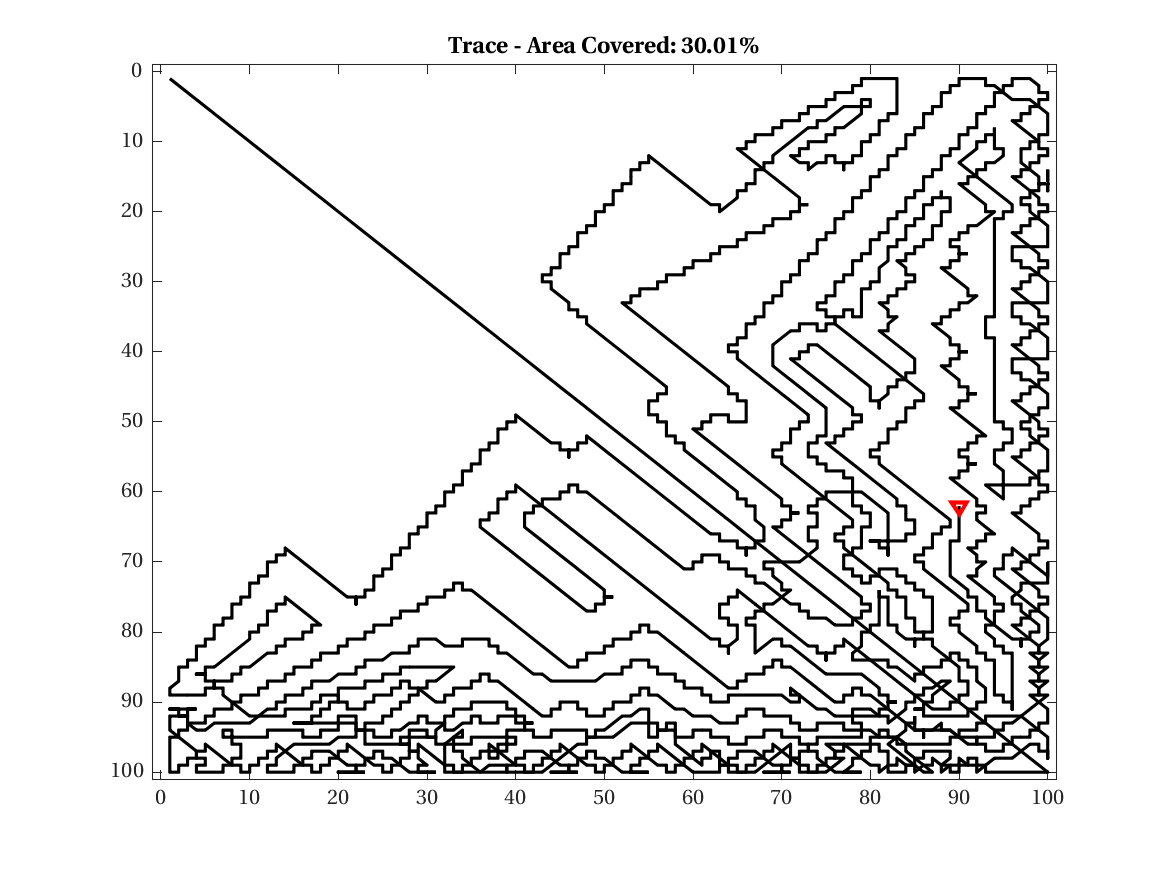
\includegraphics[width=\linewidth]{figures/hbresults/path_gradient_30p_100x100_sf_100_seed_2.png}
        \captionsetup{skip=0.20\baselineskip,size=footnotesize}
        \caption{Gradient Ascent}
    \end{subfigure}%
    \begin{subfigure}[t]{0.3333\textwidth}
        \centering
        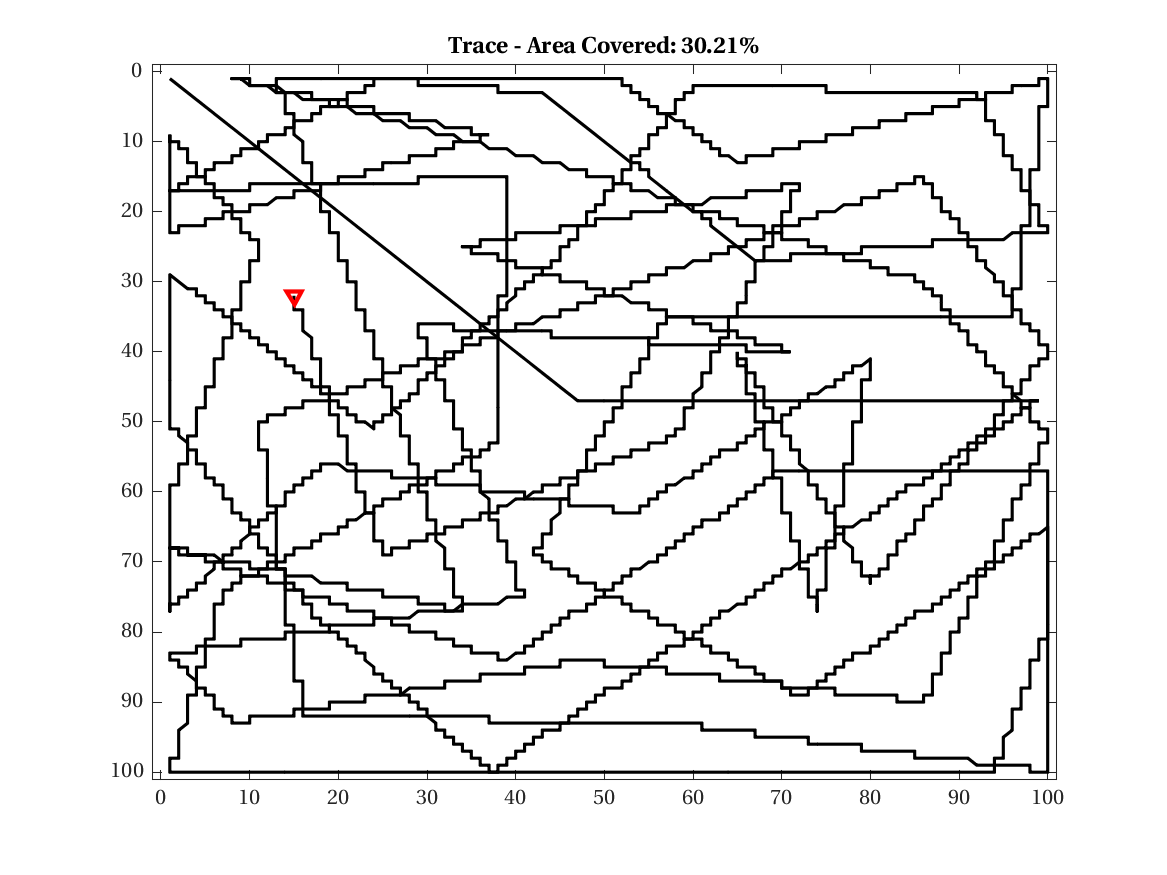
\includegraphics[width=\linewidth]{figures/hbresults/path_gr_30p_100x100_sf_100_seed_2.png}
        \captionsetup{skip=0.20\baselineskip,size=footnotesize}
        \caption{Gradient Range Ascent}
    \end{subfigure}%
    \\
    \begin{subfigure}[t]{0.3333\textwidth}
        \centering
        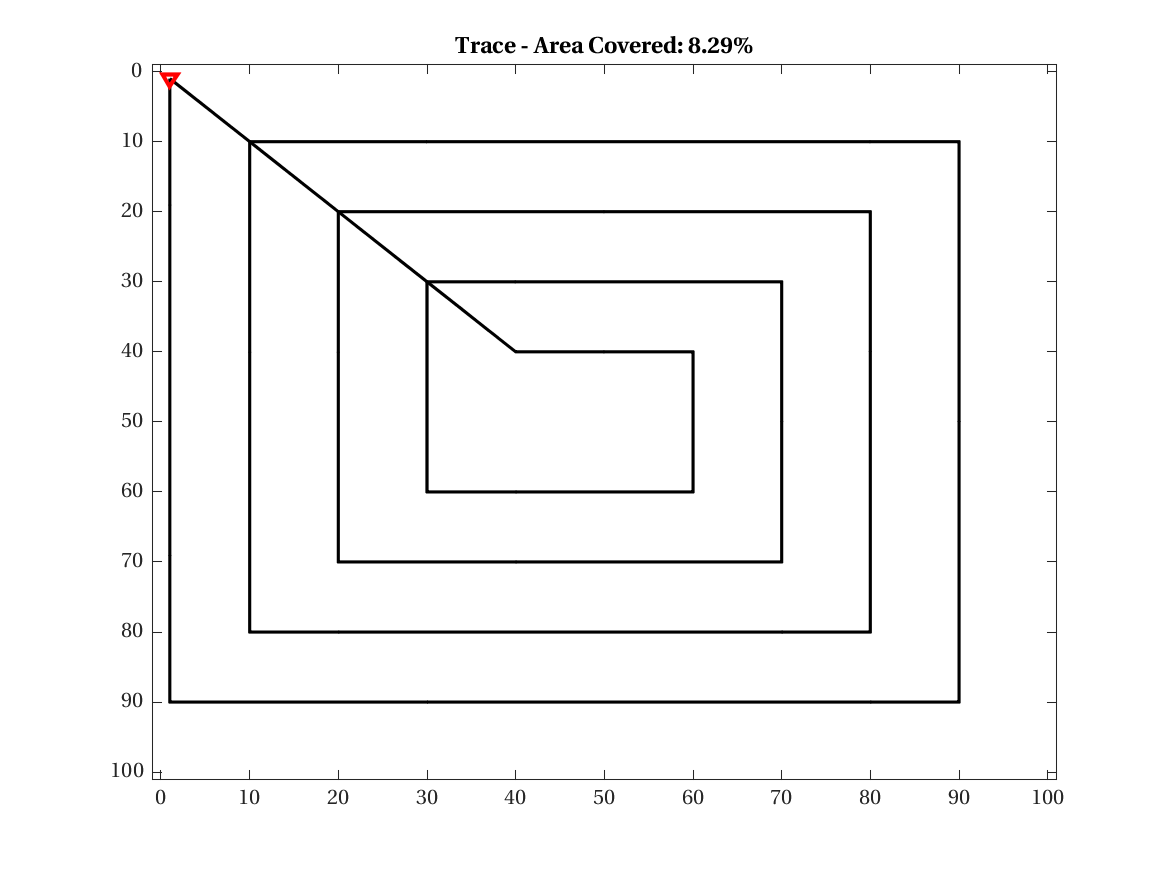
\includegraphics[width=\linewidth]{figures/hbresults/path_zz_10p_100x100_sf_100_seed_2.png}
        \captionsetup{skip=0.20\baselineskip,size=footnotesize}
        \caption{$ZZ_{10}$}
    \end{subfigure}%
    \begin{subfigure}[t]{0.3333\textwidth}
        \centering
        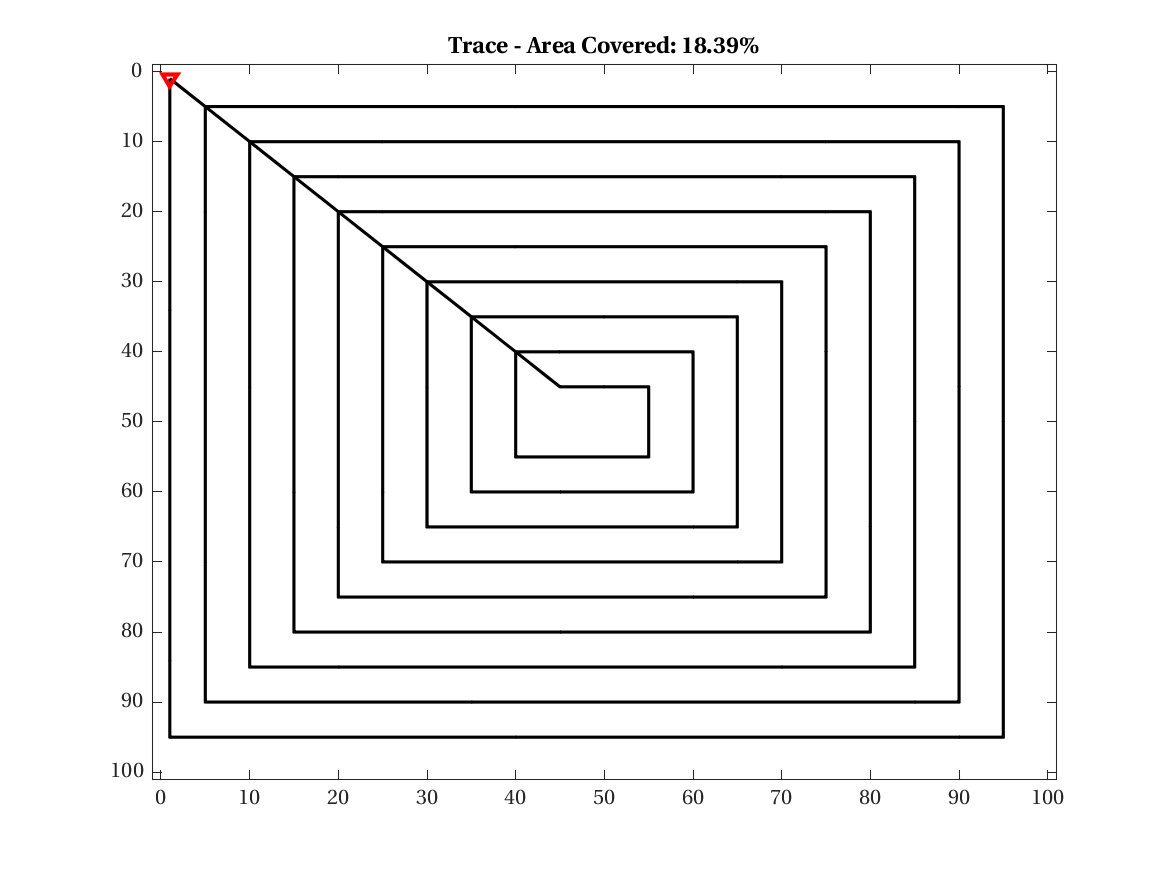
\includegraphics[width=\linewidth]{figures/hbresults/path_zz_20p_100x100_sf_100_seed_2.png}
        \captionsetup{skip=0.20\baselineskip,size=footnotesize}
        \caption{$ZZ_{20}$}
    \end{subfigure}%
    \begin{subfigure}[t]{0.3333\textwidth}
        \centering
        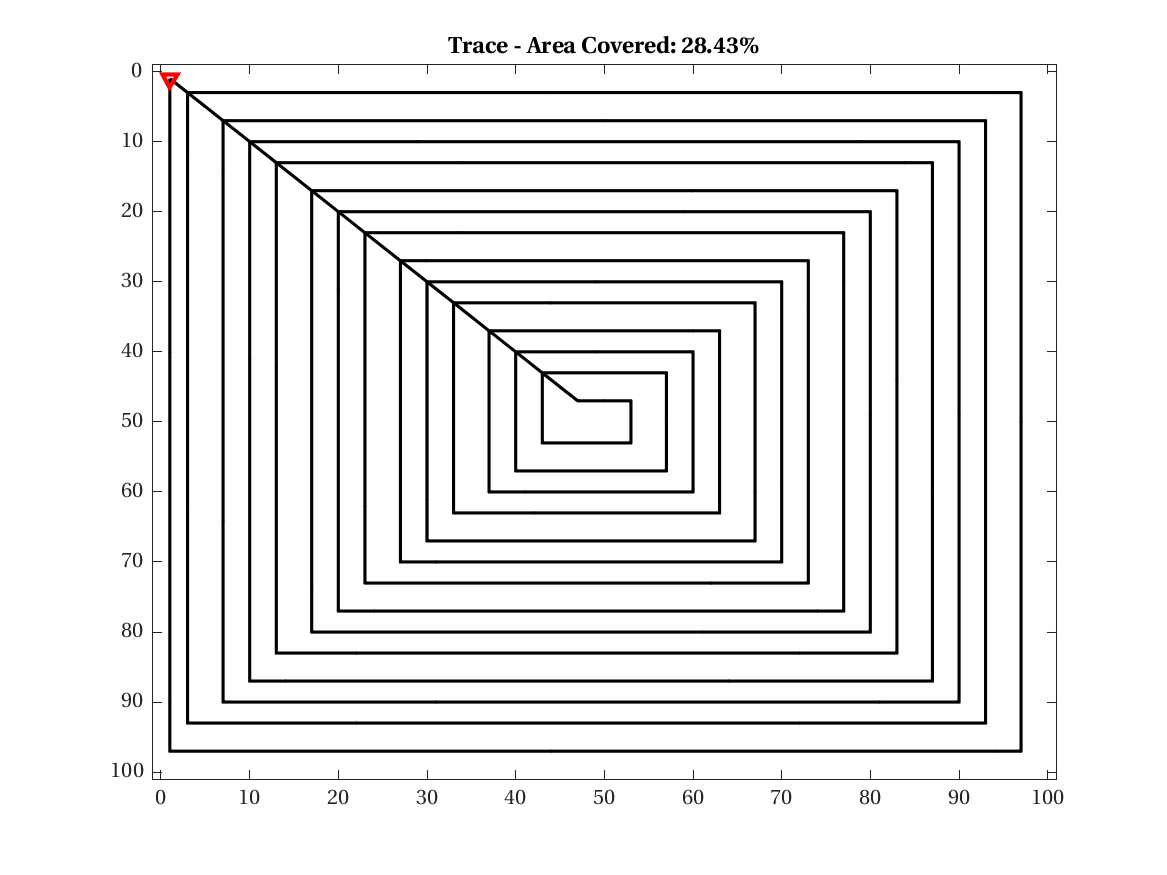
\includegraphics[width=\linewidth]{figures/hbresults/path_zz_30p_100x100_sf_100_seed_2.png}
        \captionsetup{skip=0.20\baselineskip,size=footnotesize}
        \caption{$ZZ_{30}$}
    \end{subfigure}%
    \captionsetup{skip=0.20\baselineskip}
    \caption{Exploration of a field of size $100 \times 100$, $\sigma_{field} = 100$, random seed 2.}
    \label{fig:sf100}
\end{figure}

\begin{figure}[htb!]
    \centering
    \begin{subfigure}[t]{0.75\textwidth}
        \centering
        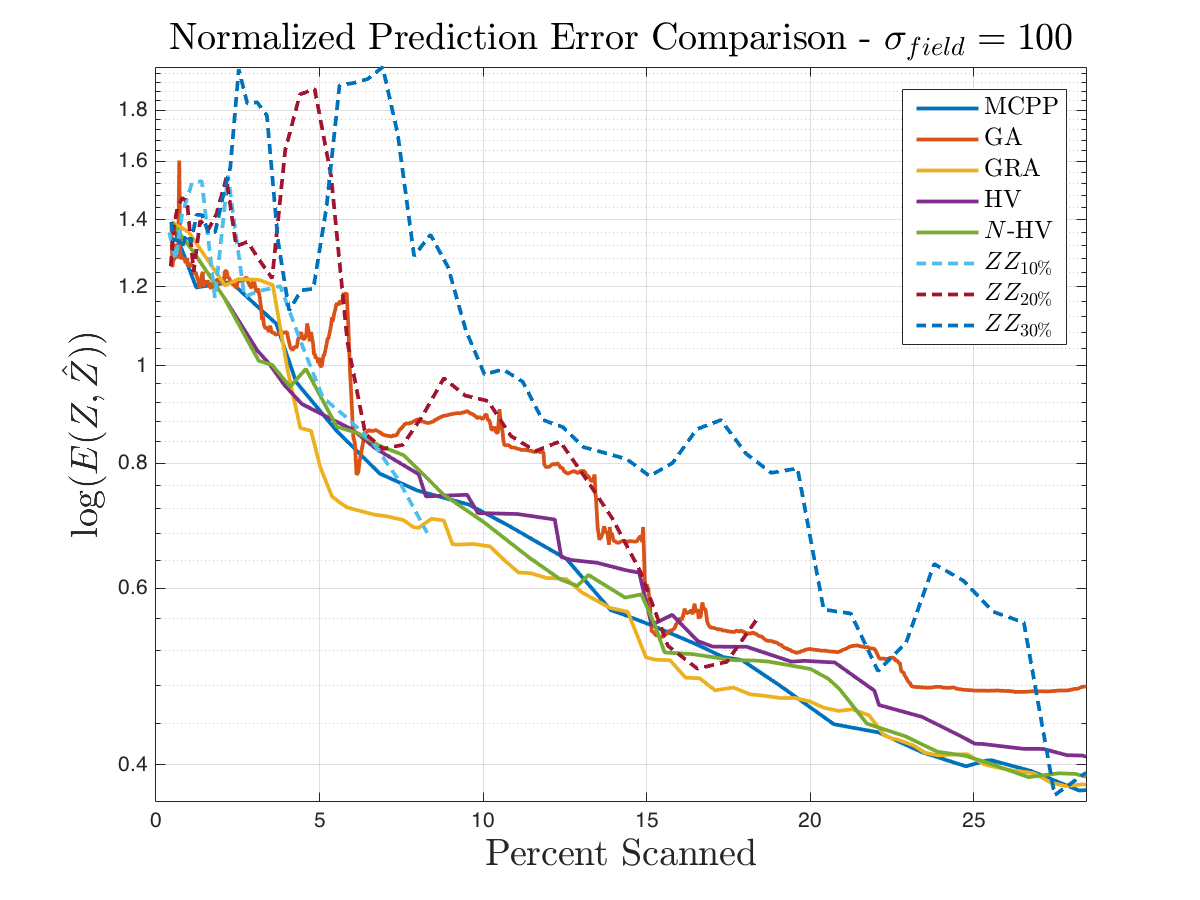
\includegraphics[width=\linewidth]{figures/results/normalized_errors_30p_100x100_sf_100_seed_2_app_50.png}
        \captionsetup{skip=0.20\baselineskip,size=footnotesize}
        \caption{Normalized prediction errors for each method.}
    \end{subfigure}%
    \\
    \begin{subfigure}[t]{0.75\textwidth}
        \centering
        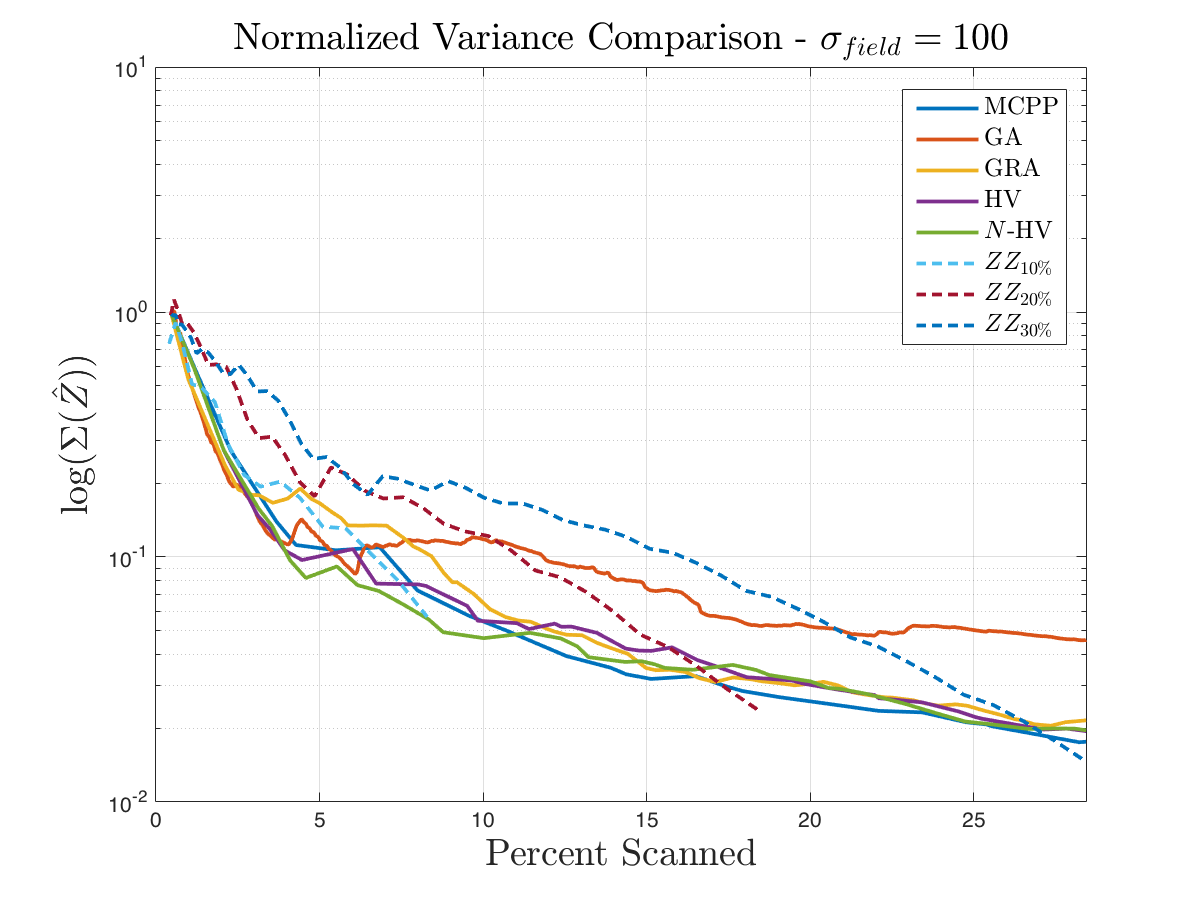
\includegraphics[width=\linewidth]{figures/results/normalized_variances_30p_100x100_sf_100_seed_2_app_50.png}
        \captionsetup{skip=0.20\baselineskip,size=footnotesize}
        \caption{Normalized prediction variances for each method.}
    \end{subfigure}%
    \captionsetup{skip=0.20\baselineskip}
    \caption{Prediction error and variances for an exploration of a field of size $100 \times 100$, $\sigma_{field} = 100$, random seed 2.}
    \label{fig:errvar100}
\end{figure}

\FloatBarrier
\clearpage

\section{Half Width Spatial Autocorrelation Results}
The methods will be compared on target fields generated with an autocorrelation factor, $\sigma_{field}$, equal to the half of the target field's width. A Gaussian filter $G(x,y,50)$ (Equation \ref{eq:gauss_filt}), is convolved with all points on the field.

\begin{figure}[htb!]
    \centering
    \begin{subfigure}[t]{0.3333\textwidth}
        \centering
        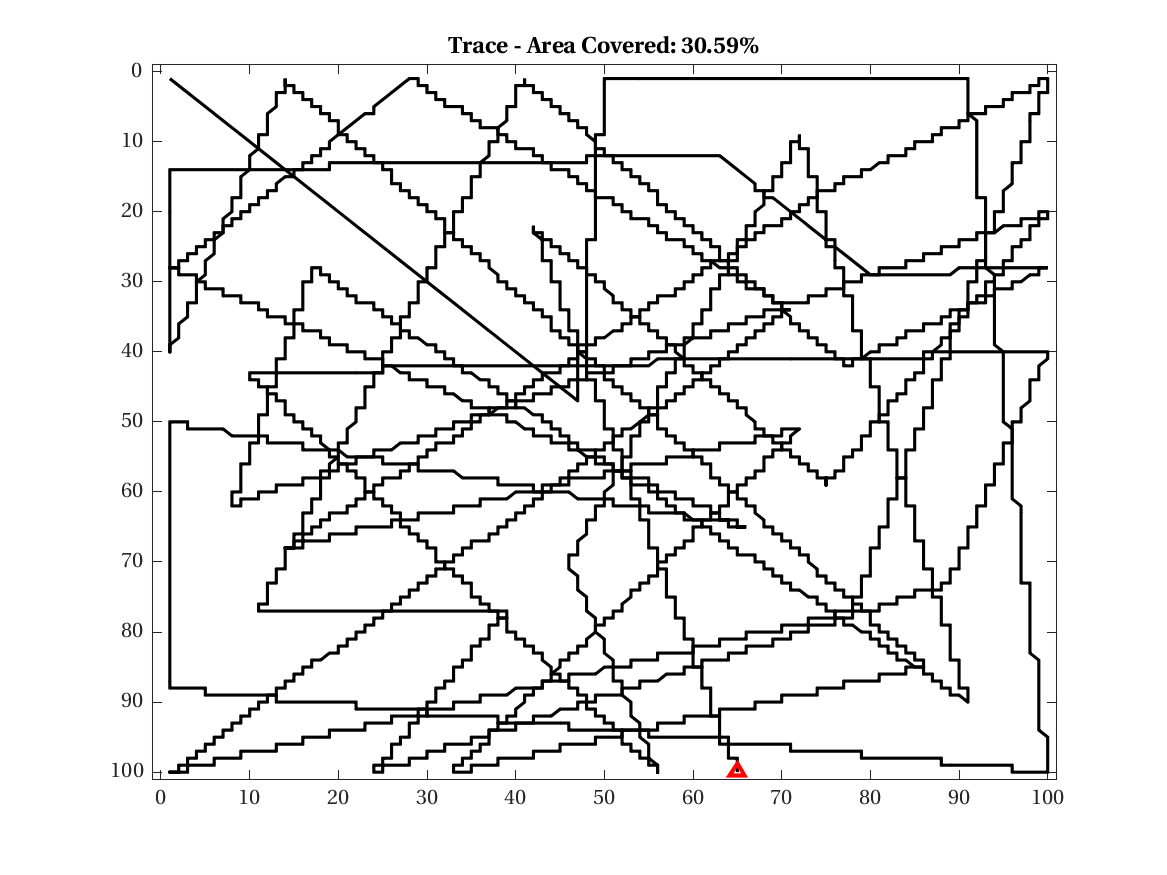
\includegraphics[width=\linewidth]{figures/hbresults/path_nhv_30p_100x100_sf_50_seed_2.png}
        \captionsetup{skip=0.20\baselineskip,size=footnotesize}
        \caption{Highest Variance}
    \end{subfigure}%
    \begin{subfigure}[t]{0.3333\textwidth}
        \centering
        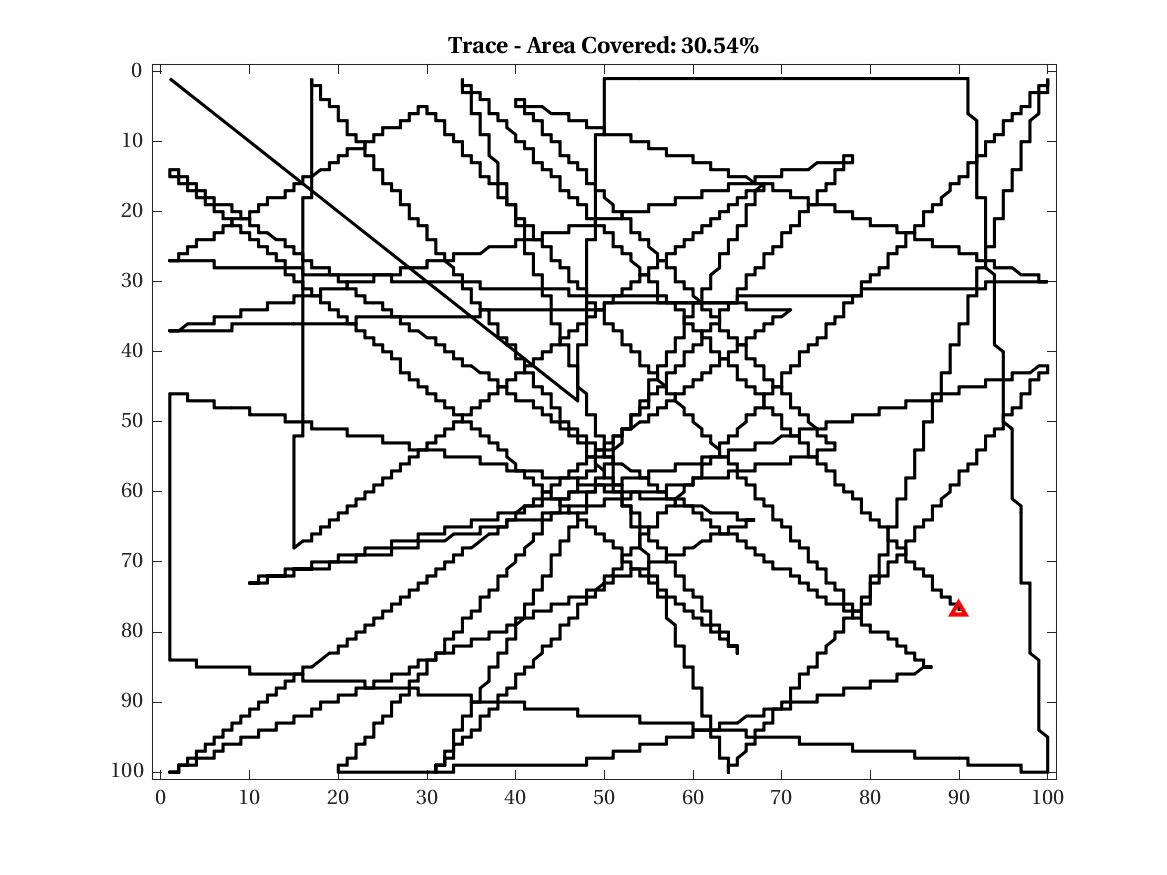
\includegraphics[width=\linewidth]{figures/hbresults/path_nnhv_30p_100x100_sf_50_seed_2.png}
        \captionsetup{skip=0.20\baselineskip,size=footnotesize}
        \caption{$N$ Highest Variance}
    \end{subfigure}%
    \begin{subfigure}[t]{0.3333\textwidth}
        \centering
        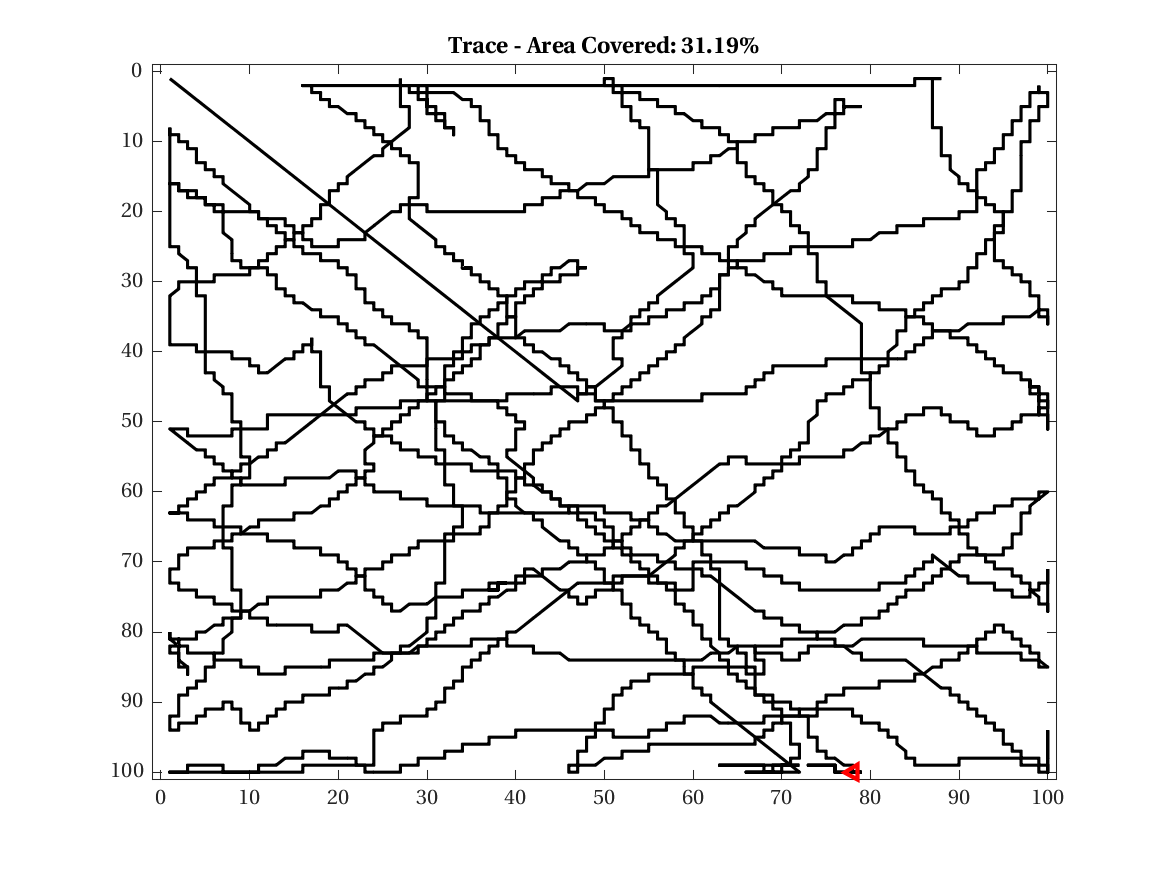
\includegraphics[width=\linewidth]{figures/hbresults/path_mc_30p_100x100_sf_50_seed_2.png}
        \captionsetup{skip=0.20\baselineskip,size=footnotesize}
        \caption{Monte Carlo}
    \end{subfigure}%
    \\
    \begin{subfigure}[t]{0.3333\textwidth}
        \centering
        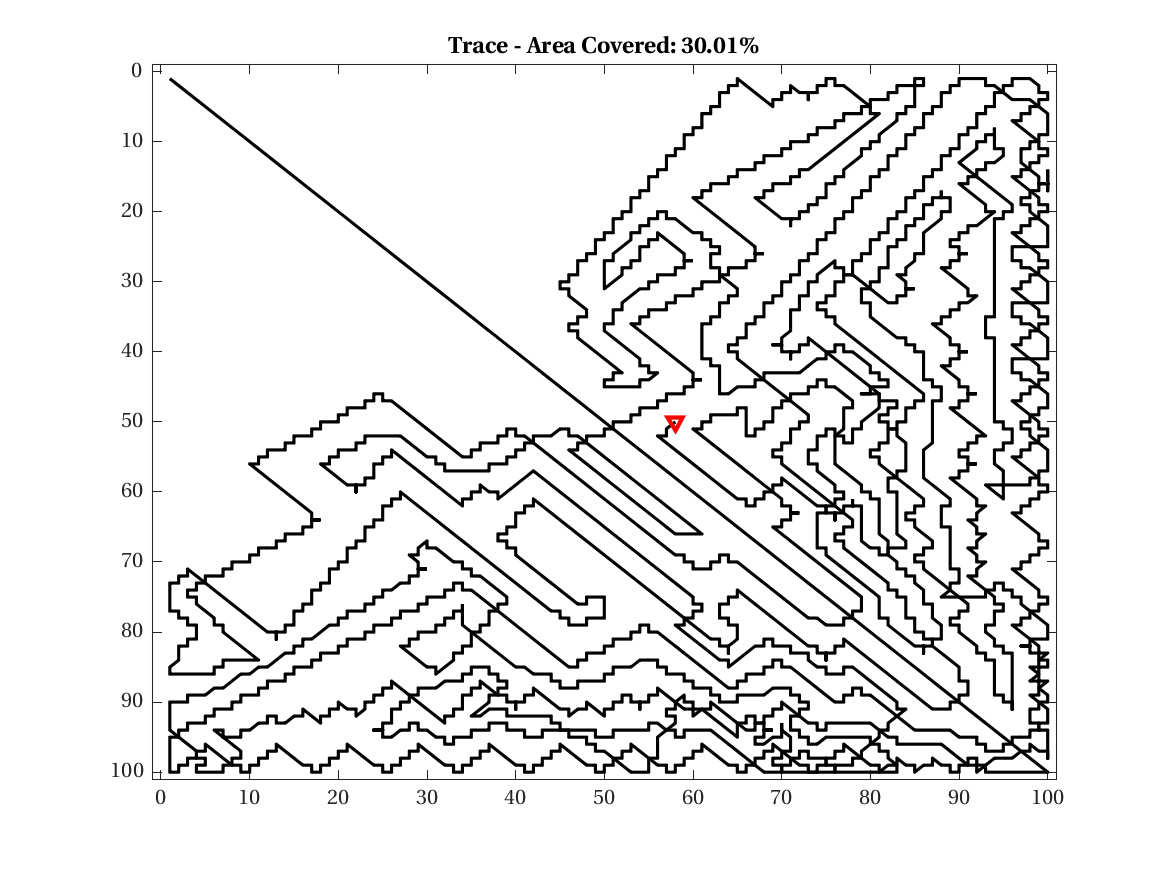
\includegraphics[width=\linewidth]{figures/hbresults/path_gradient_30p_100x100_sf_50_seed_2.png}
        \captionsetup{skip=0.20\baselineskip,size=footnotesize}
        \caption{Gradient Ascent}
    \end{subfigure}%
    \begin{subfigure}[t]{0.3333\textwidth}
        \centering
        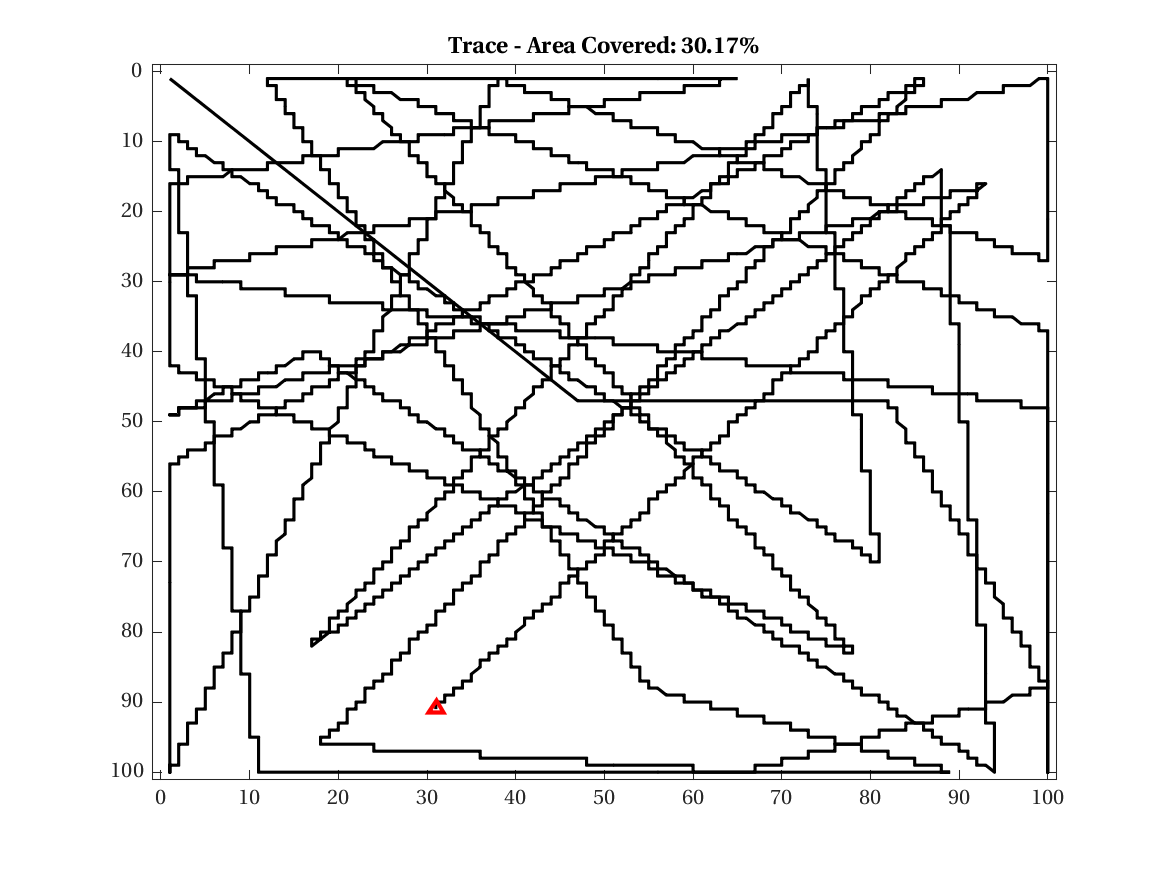
\includegraphics[width=\linewidth]{figures/hbresults/path_gr_30p_100x100_sf_50_seed_2.png}
        \captionsetup{skip=0.20\baselineskip,size=footnotesize}
        \caption{Gradient Range Ascent}
    \end{subfigure}%
    \\
    \begin{subfigure}[t]{0.3333\textwidth}
        \centering
        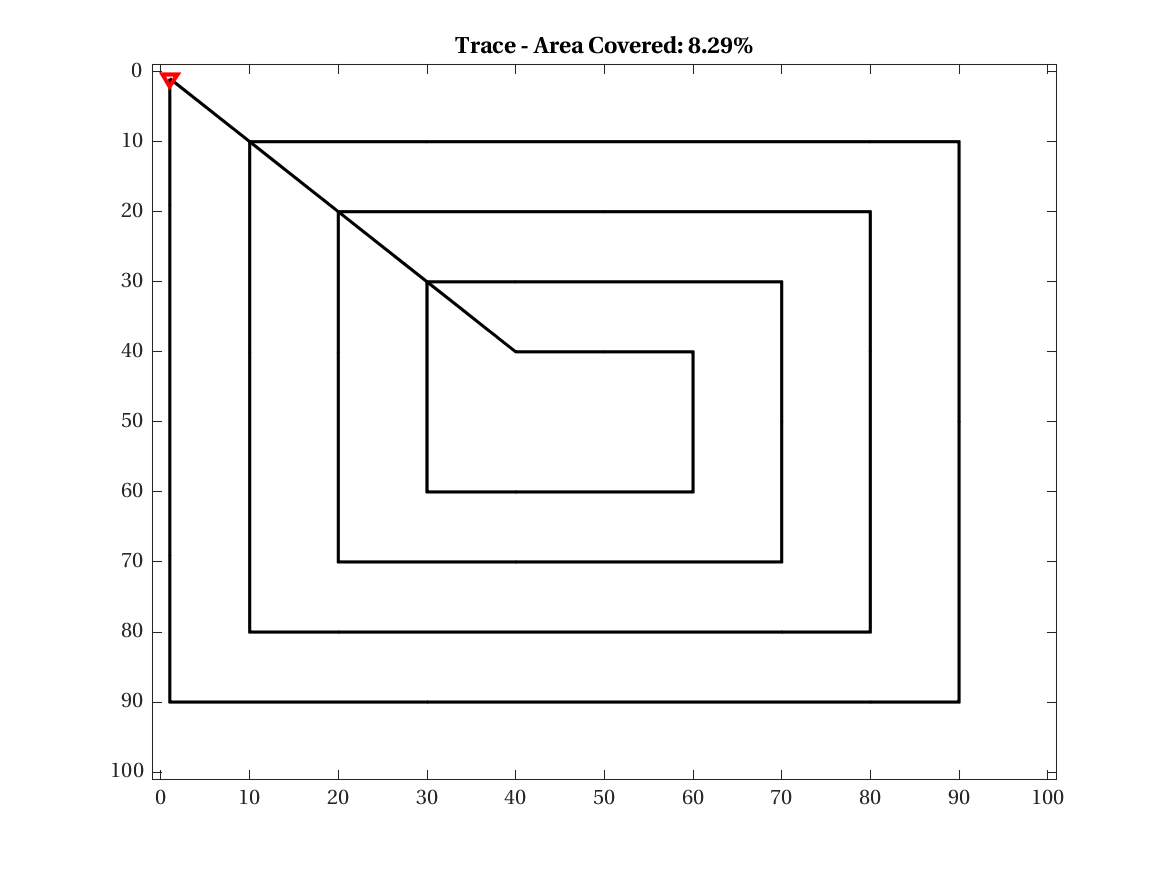
\includegraphics[width=\linewidth]{figures/hbresults/path_zz_10p_100x100_sf_50_seed_2.png}
        \captionsetup{skip=0.20\baselineskip,size=footnotesize}
        \caption{$ZZ_{10}$}
    \end{subfigure}%
    \begin{subfigure}[t]{0.3333\textwidth}
        \centering
        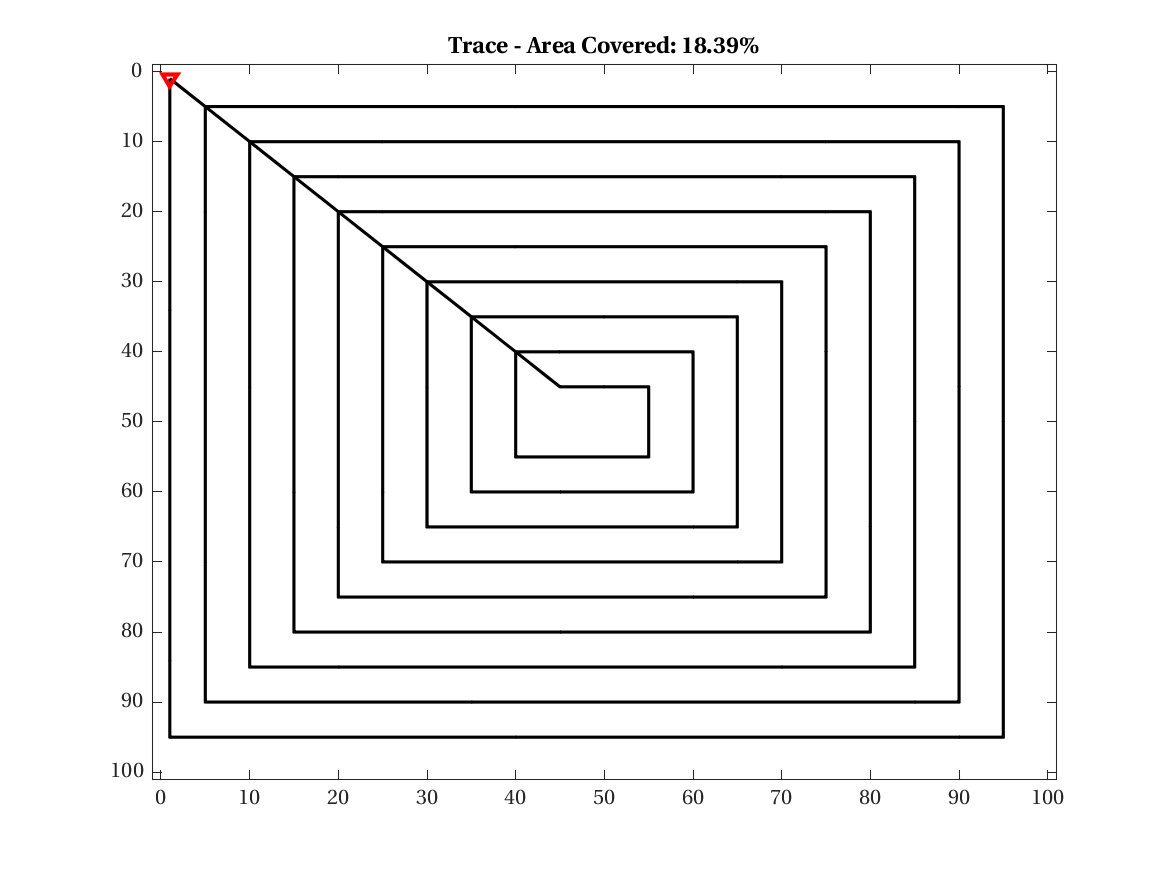
\includegraphics[width=\linewidth]{figures/hbresults/path_zz_20p_100x100_sf_50_seed_2.png}
        \captionsetup{skip=0.20\baselineskip,size=footnotesize}
        \caption{$ZZ_{20}$}
    \end{subfigure}%
    \begin{subfigure}[t]{0.3333\textwidth}
        \centering
        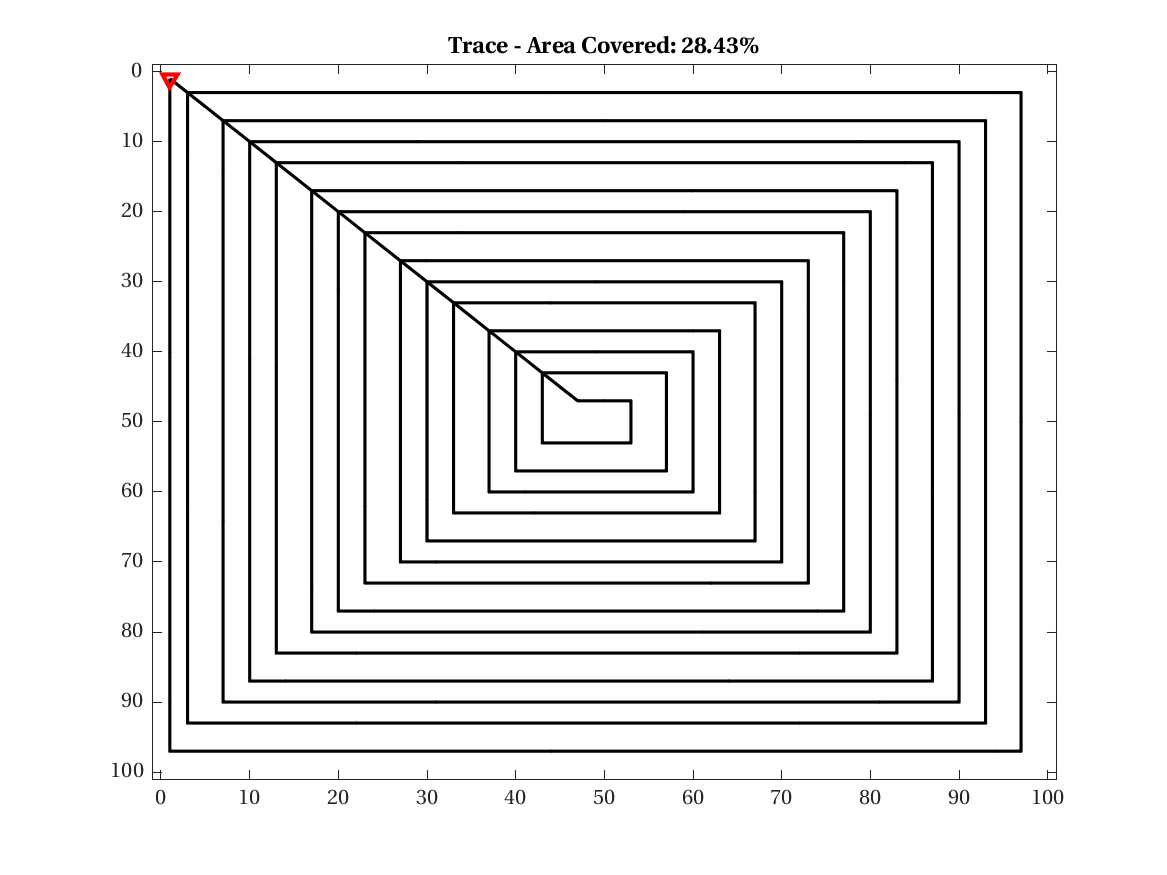
\includegraphics[width=\linewidth]{figures/hbresults/path_zz_30p_100x100_sf_50_seed_2.png}
        \captionsetup{skip=0.20\baselineskip,size=footnotesize}
        \caption{$ZZ_{30}$}
    \end{subfigure}%
    \captionsetup{skip=0.20\baselineskip}
    \caption{Exploration of a field of size $100 \times 100$, $\sigma_{field} = \frac{w}{2} = 50$, random seed 2.}
    \label{fig:sf50}
\end{figure}

\begin{figure}[htb!]
    \centering
    \begin{subfigure}[t]{0.75\textwidth}
        \centering
        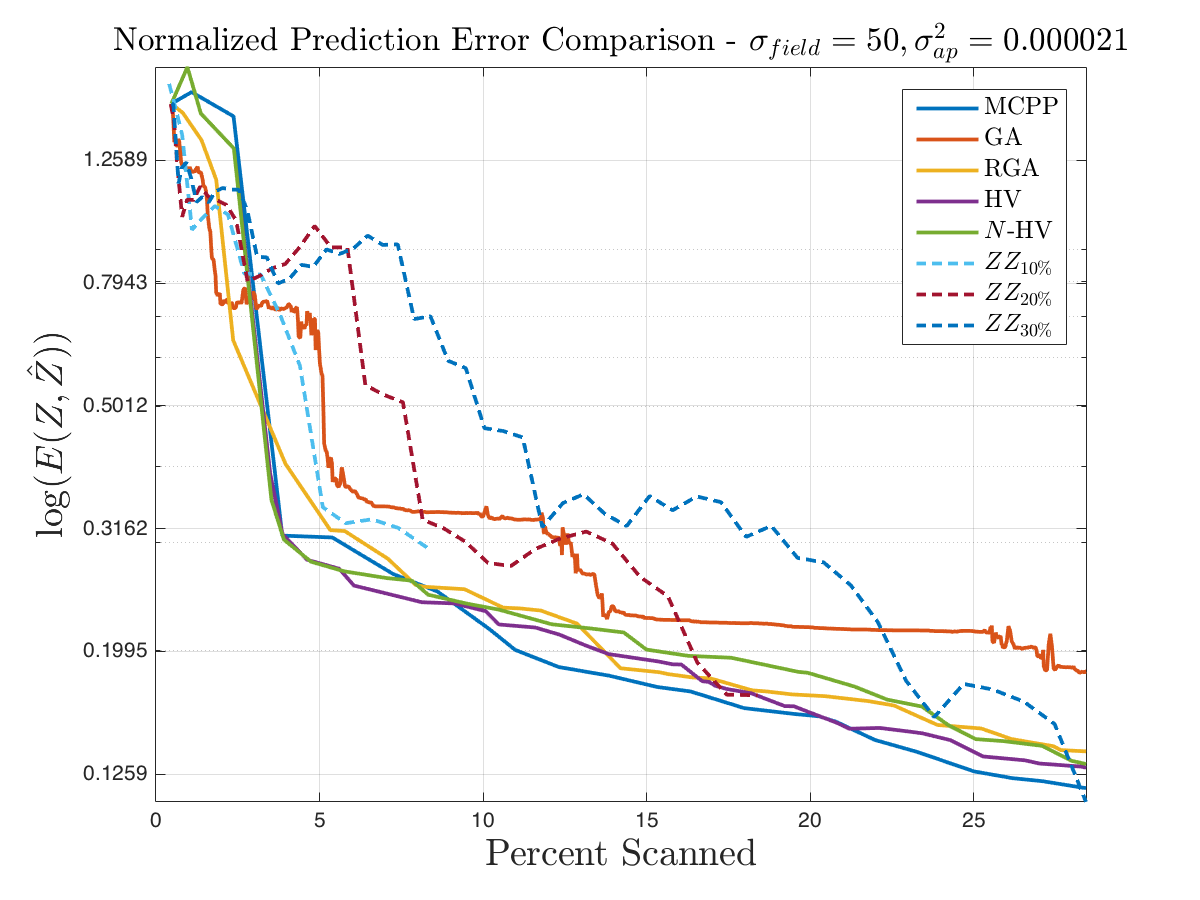
\includegraphics[width=\linewidth]{figures/results/normalized_errors_30p_100x100_sf_50_seed_2_app_50.png}
        \captionsetup{skip=0.20\baselineskip,size=footnotesize}
        \caption{Normalized prediction errors for each method.}
    \end{subfigure}%
    \\
    \begin{subfigure}[t]{0.75\textwidth}
        \centering
        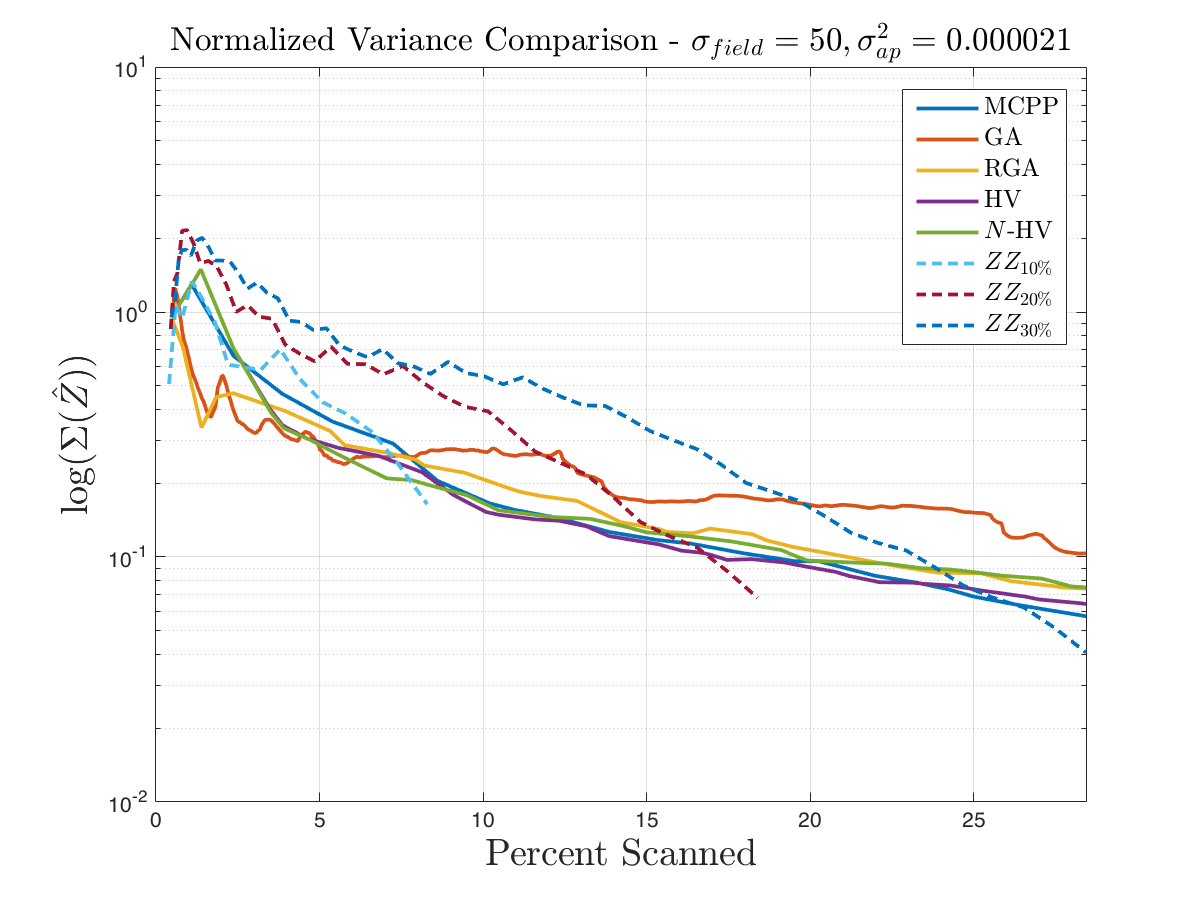
\includegraphics[width=\linewidth]{figures/results/normalized_variances_30p_100x100_sf_50_seed_2_app_50.png}
        \captionsetup{skip=0.20\baselineskip,size=footnotesize}
        \caption{Normalized prediction variances for each method.}
    \end{subfigure}%
    \captionsetup{skip=0.20\baselineskip}
    \caption{Prediction error and variances for an exploration of a field of size $100 \times 100$, $\sigma_{field} = 50$, random seed 2.}
    \label{fig:errvar50}
\end{figure}

\FloatBarrier
\clearpage

\section{Low Spatial Autocorrelation Results}
The methods will be compared on target fields generated with an autocorrelation factor, $\sigma_{field}$, equal to one. A Gaussian filter $G(x,y,1)$ (Equation \ref{eq:gauss_filt}), is convolved with all points on the field.

\begin{figure}[htb!]
    \centering
    \begin{subfigure}[t]{0.3333\textwidth}
        \centering
        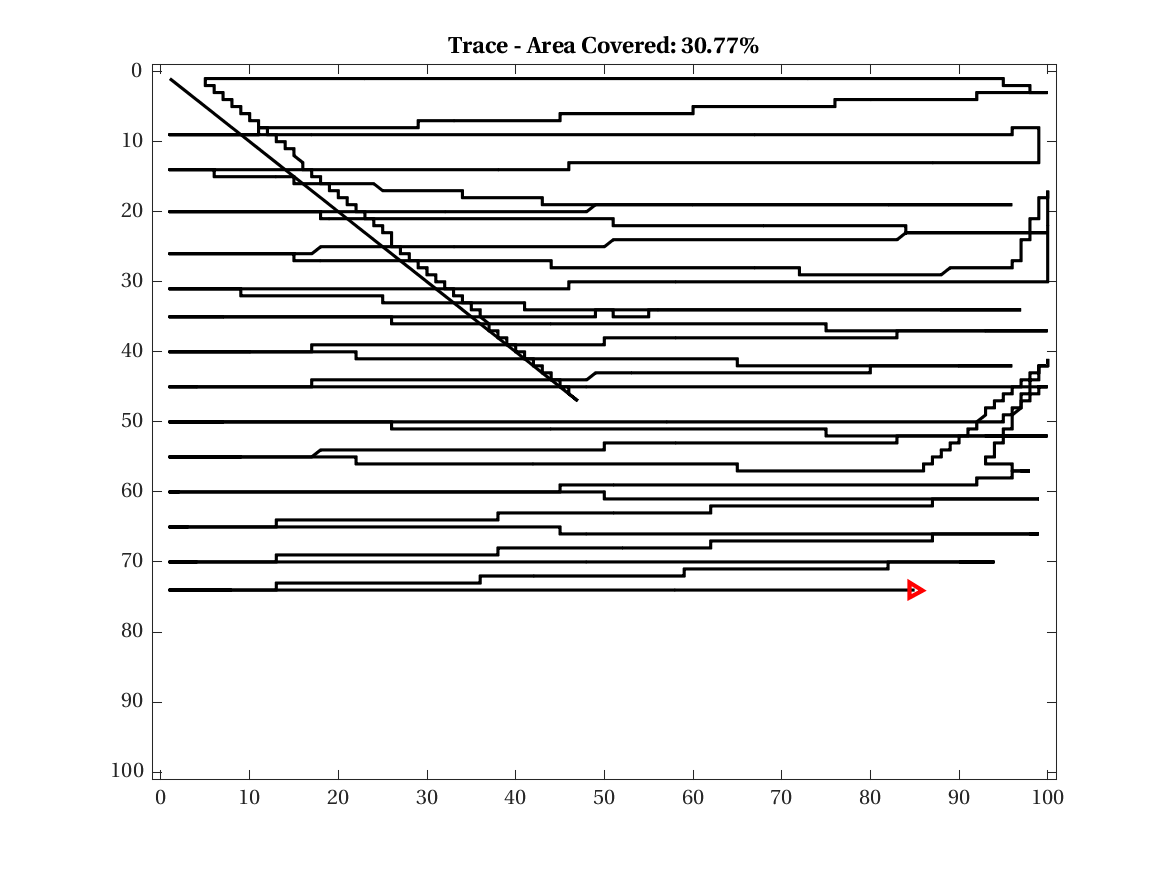
\includegraphics[width=\linewidth]{figures/hbresults/path_nhv_30p_100x100_sf_1_seed_2.png}
        \captionsetup{skip=0.20\baselineskip,size=footnotesize}
        \caption{Highest Variance}
    \end{subfigure}%
    \begin{subfigure}[t]{0.3333\textwidth}
        \centering
        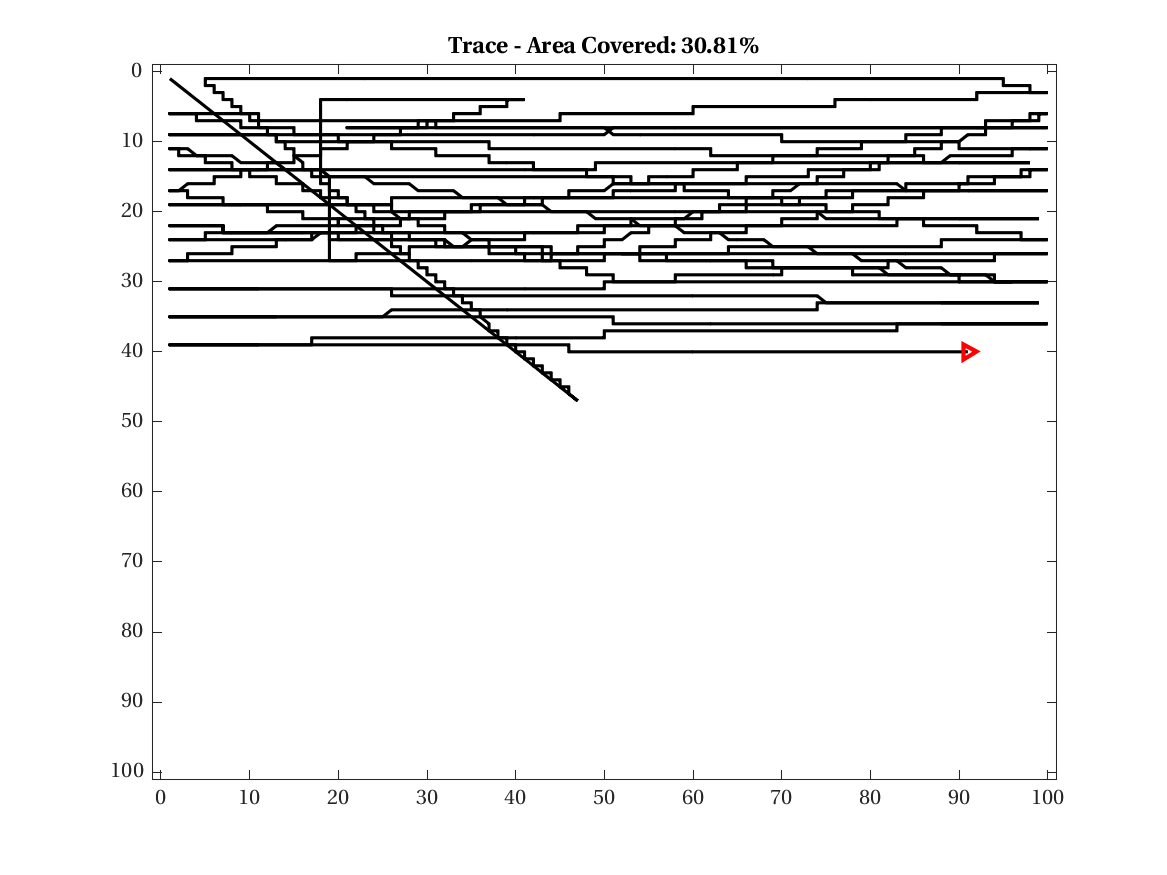
\includegraphics[width=\linewidth]{figures/hbresults/path_nnhv_30p_100x100_sf_1_seed_2.png}
        \captionsetup{skip=0.20\baselineskip,size=footnotesize}
        \caption{$N$ Highest Variance}
    \end{subfigure}%
    \begin{subfigure}[t]{0.3333\textwidth}
        \centering
        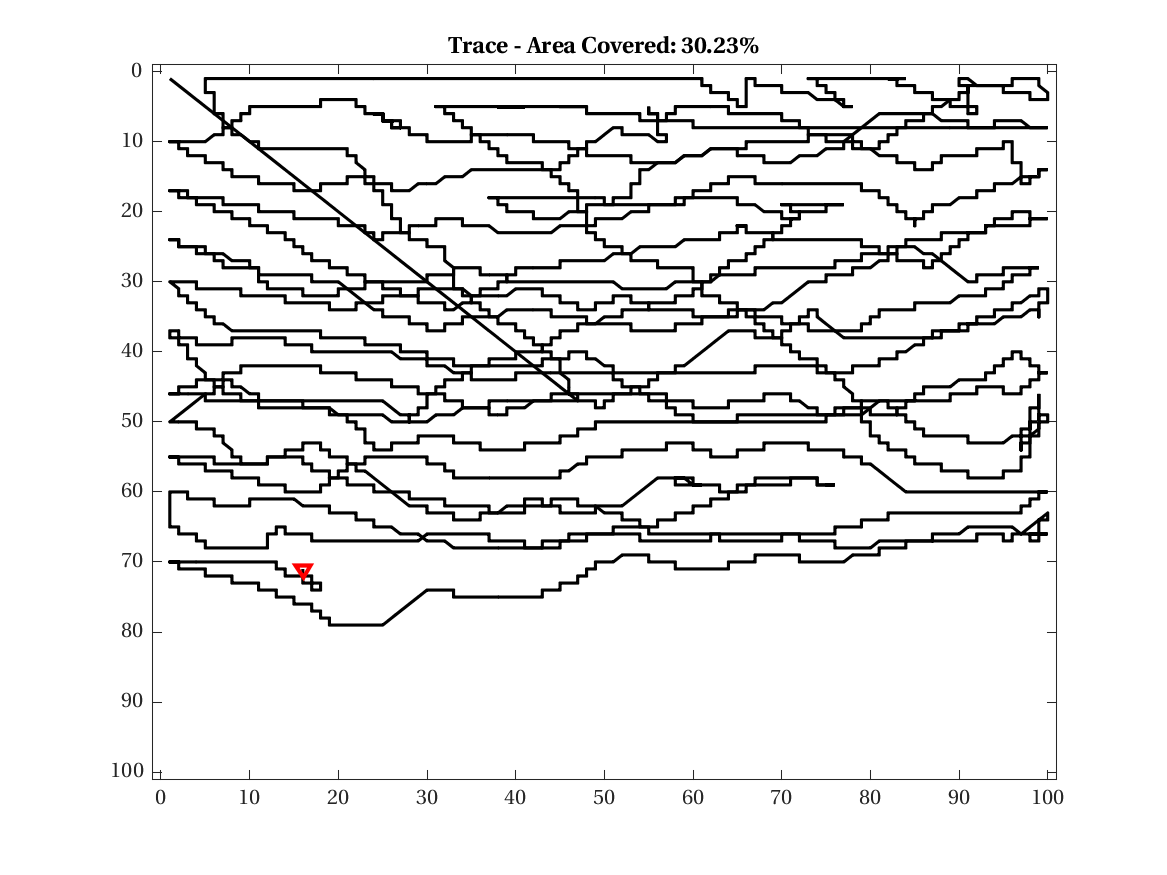
\includegraphics[width=\linewidth]{figures/hbresults/path_mc_30p_100x100_sf_1_seed_2.png}
        \captionsetup{skip=0.20\baselineskip,size=footnotesize}
        \caption{Monte Carlo}
    \end{subfigure}%
    \\
    \begin{subfigure}[t]{0.3333\textwidth}
        \centering
        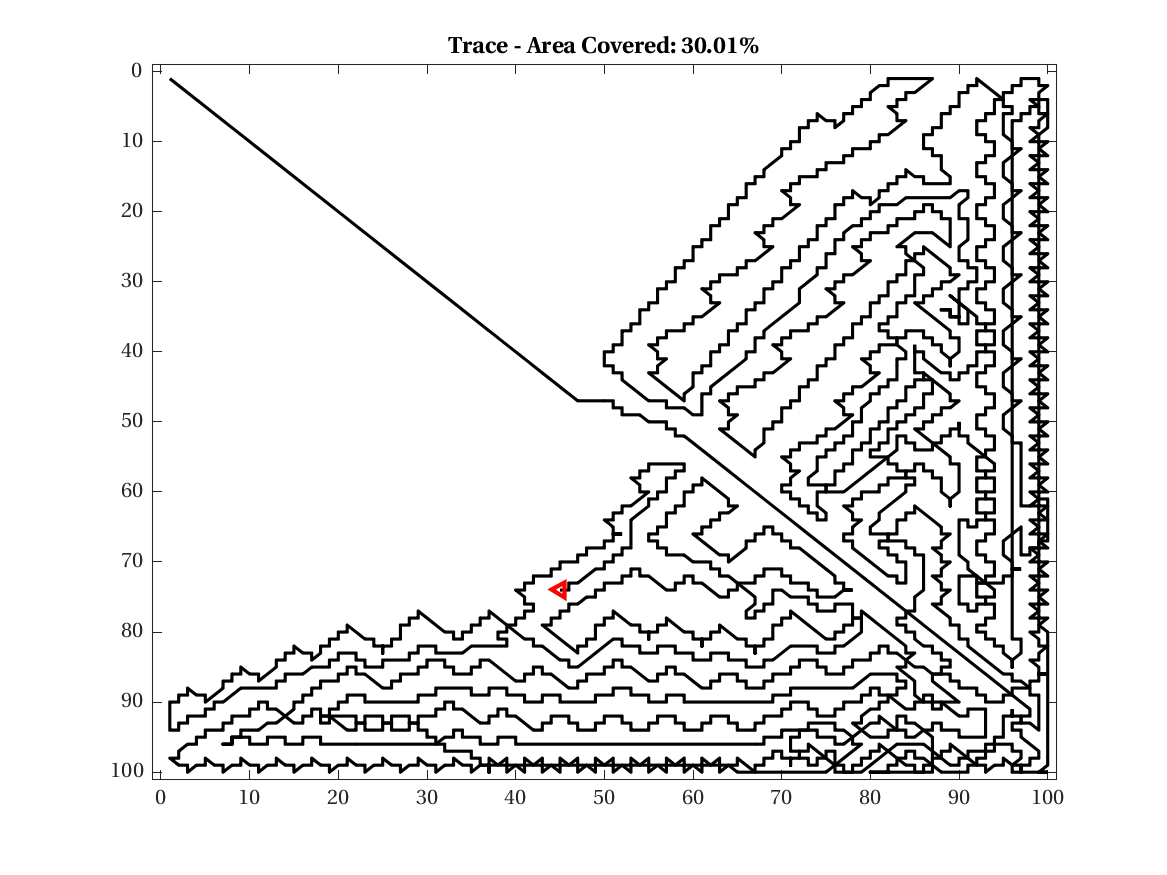
\includegraphics[width=\linewidth]{figures/hbresults/path_gradient_30p_100x100_sf_1_seed_2.png}
        \captionsetup{skip=0.20\baselineskip,size=footnotesize}
        \caption{Gradient Ascent}
    \end{subfigure}%
    \begin{subfigure}[t]{0.3333\textwidth}
        \centering
        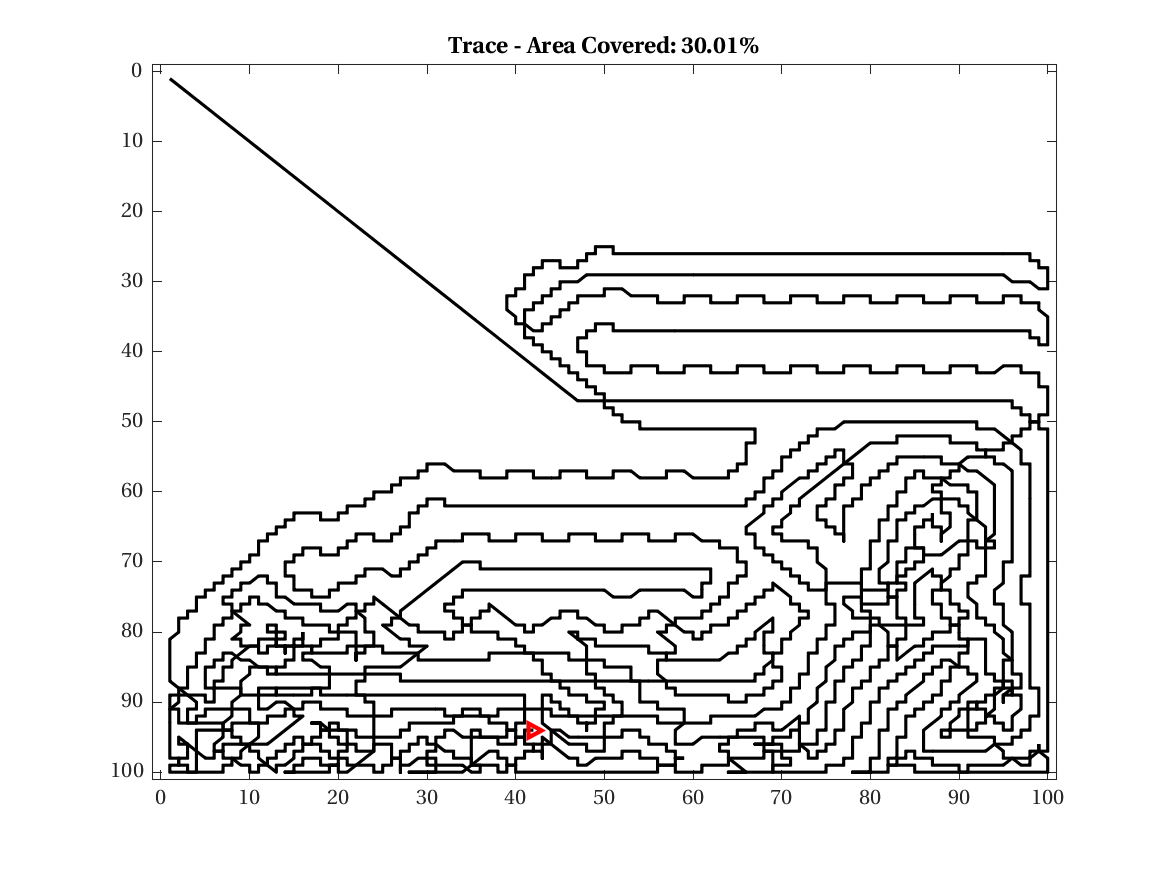
\includegraphics[width=\linewidth]{figures/hbresults/path_gr_30p_100x100_sf_1_seed_2.png}
        \captionsetup{skip=0.20\baselineskip,size=footnotesize}
        \caption{Gradient Range Ascent}
    \end{subfigure}%
    \\
    \begin{subfigure}[t]{0.3333\textwidth}
        \centering
        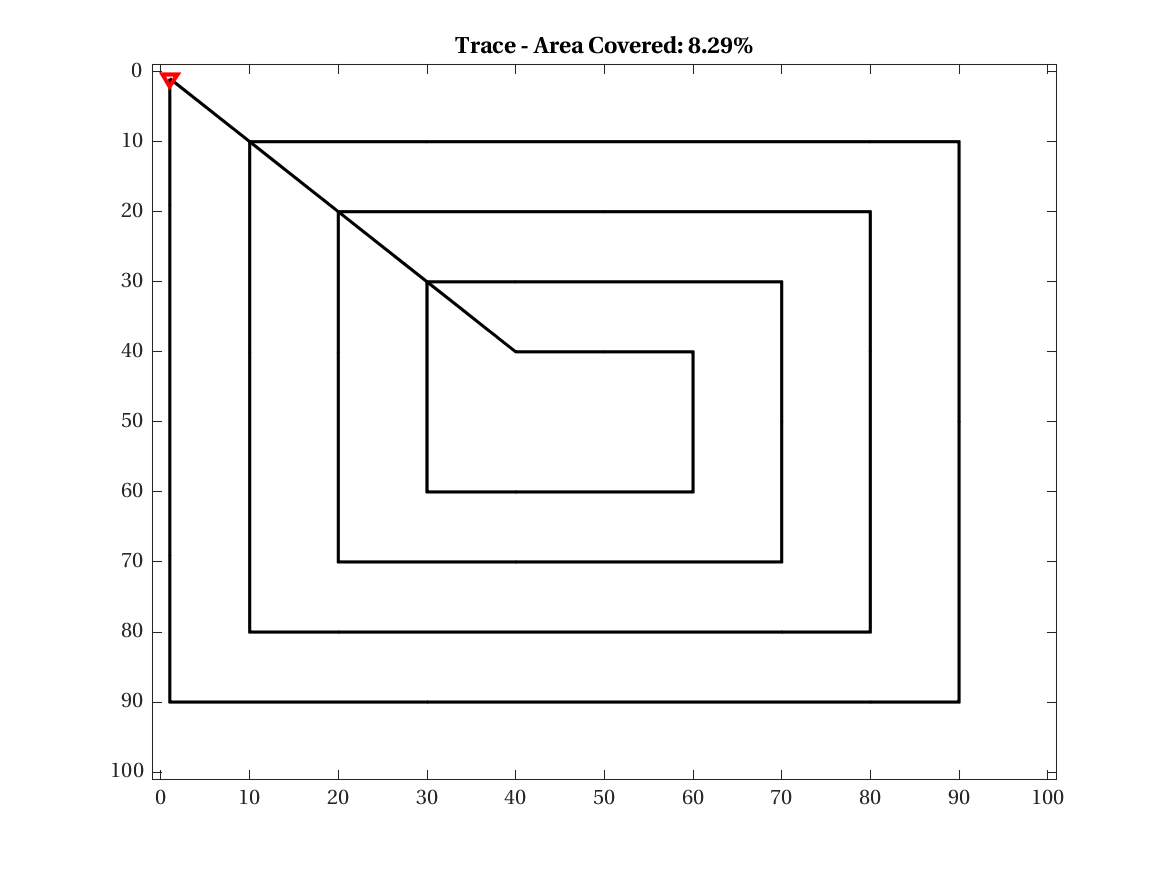
\includegraphics[width=\linewidth]{figures/hbresults/path_zz_10p_100x100_sf_1_seed_2.png}
        \captionsetup{skip=0.20\baselineskip,size=footnotesize}
        \caption{$ZZ_{10}$}
    \end{subfigure}%
    \begin{subfigure}[t]{0.3333\textwidth}
        \centering
        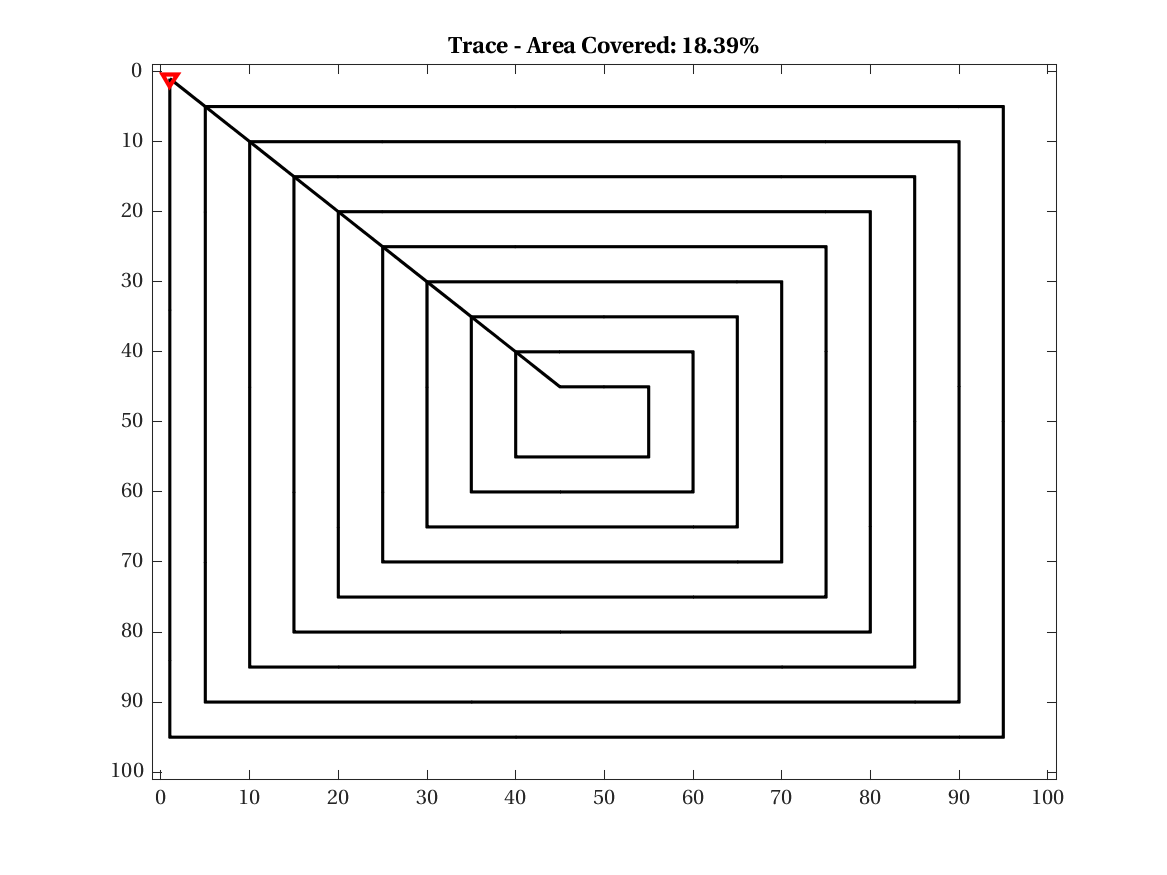
\includegraphics[width=\linewidth]{figures/hbresults/path_zz_20p_100x100_sf_1_seed_2.png}
        \captionsetup{skip=0.20\baselineskip,size=footnotesize}
        \caption{$ZZ_{20}$}
    \end{subfigure}%
    \begin{subfigure}[t]{0.3333\textwidth}
        \centering
        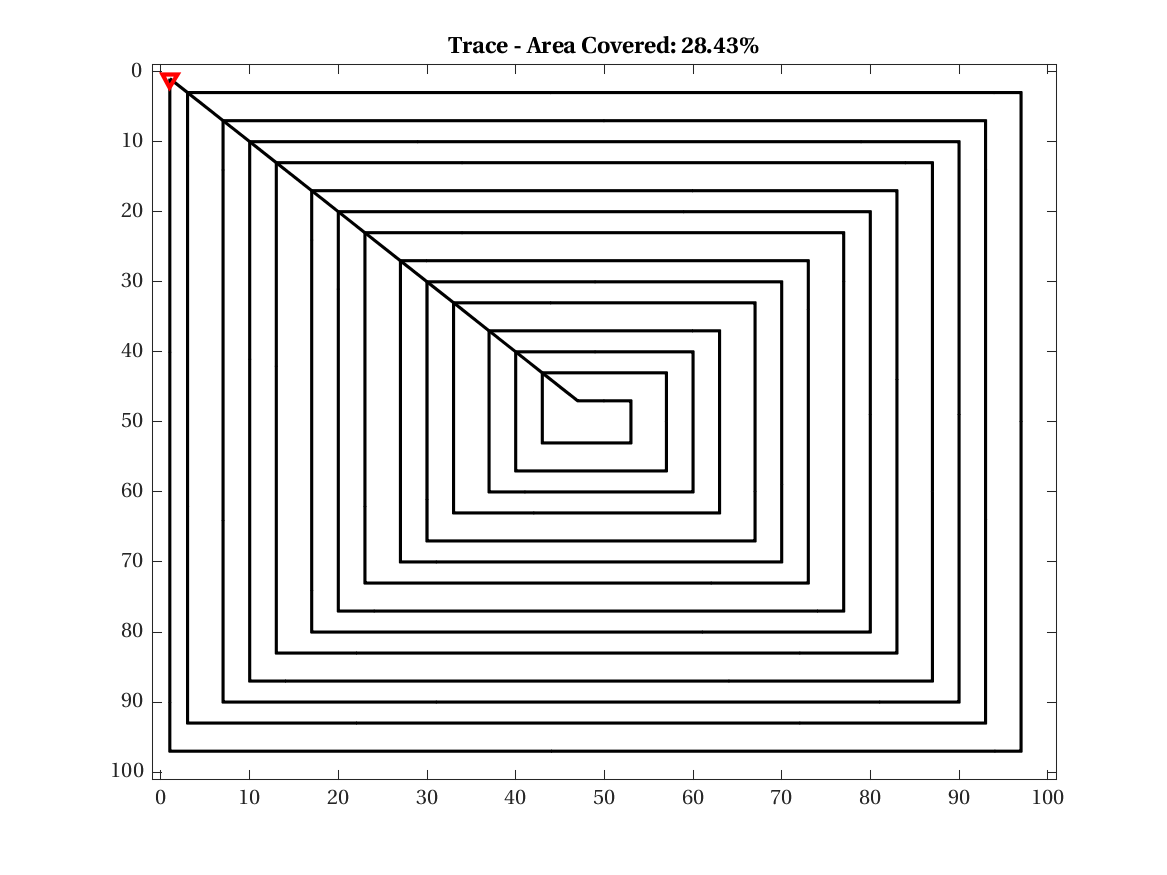
\includegraphics[width=\linewidth]{figures/hbresults/path_zz_30p_100x100_sf_1_seed_2.png}
        \captionsetup{skip=0.20\baselineskip,size=footnotesize}
        \caption{$ZZ_{30}$}
    \end{subfigure}%
    \captionsetup{skip=0.20\baselineskip}
    \caption{Exploration of a field of size $100 \times 100$, $\sigma_{field} = 1$, random seed 2.}
    \label{fig:sf1}
\end{figure}

\begin{figure}[htb!]
    \centering
    \begin{subfigure}[t]{0.75\textwidth}
        \centering
        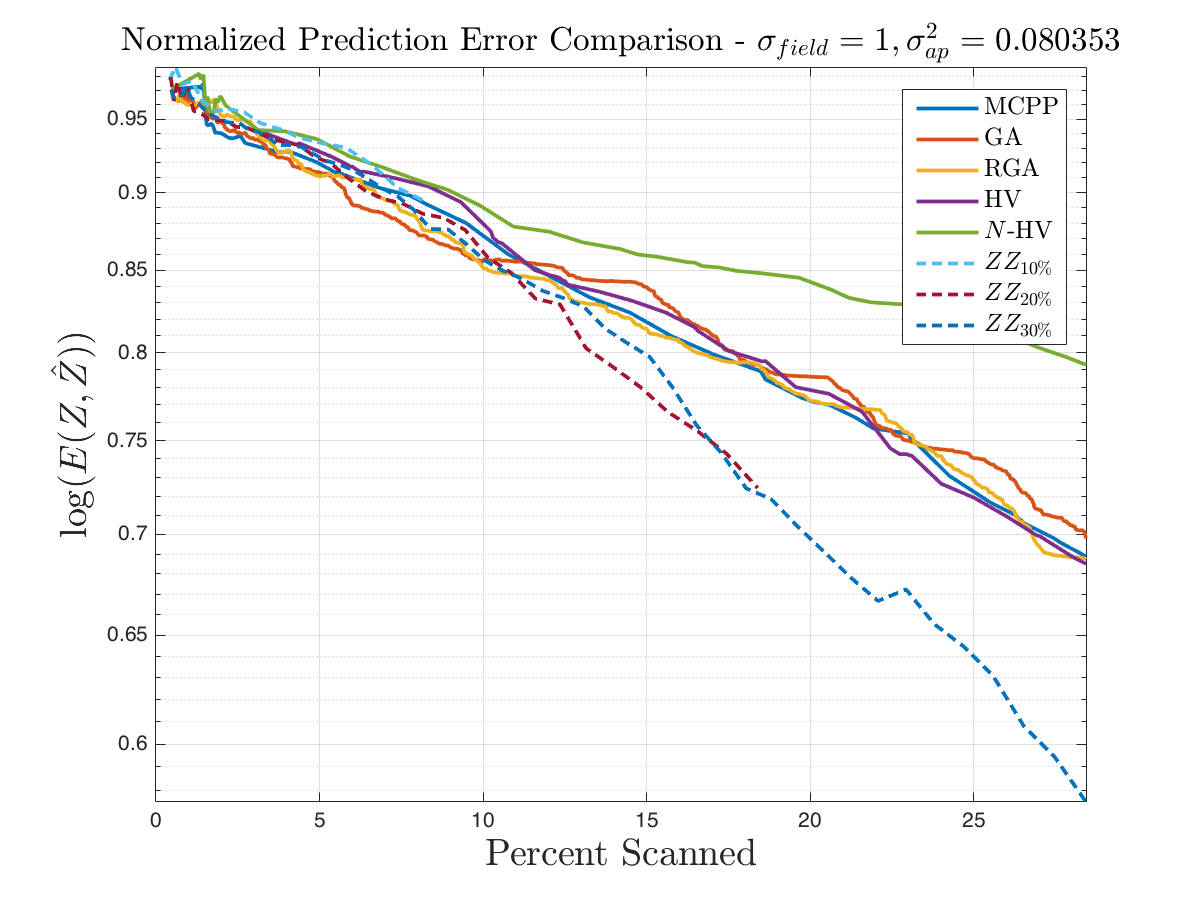
\includegraphics[width=\linewidth]{figures/results/normalized_errors_30p_100x100_sf_1_seed_2_app_50.png}
        \captionsetup{skip=0.20\baselineskip,size=footnotesize}
        \caption{Normalized prediction errors for each method.}
    \end{subfigure}%
    \\
    \begin{subfigure}[t]{0.75\textwidth}
        \centering
        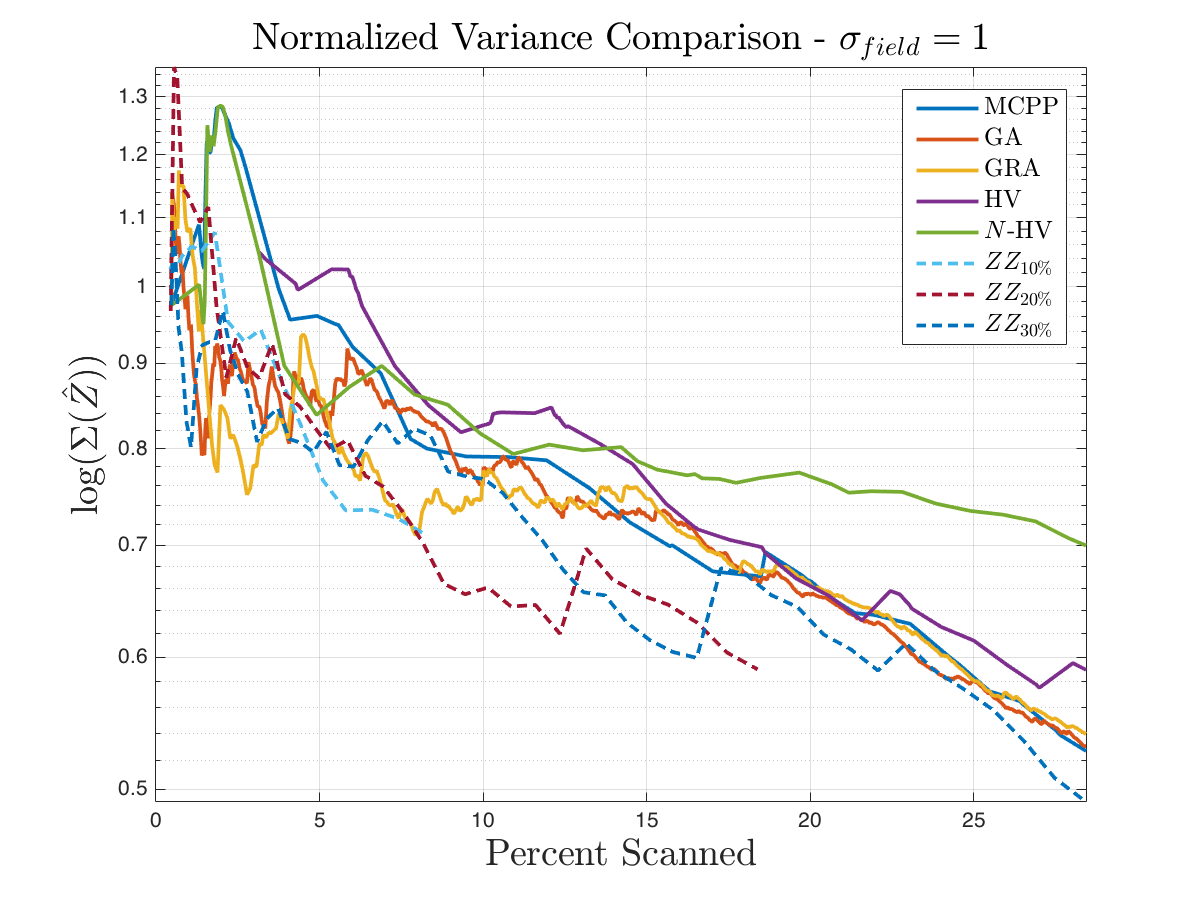
\includegraphics[width=\linewidth]{figures/results/normalized_variances_30p_100x100_sf_1_seed_2_app_50.png}
        \captionsetup{skip=0.20\baselineskip,size=footnotesize}
        \caption{Normalized prediction variances for each method.}
    \end{subfigure}%
    \captionsetup{skip=0.20\baselineskip}
    \caption{Prediction error and variances for an exploration of a field of size $100 \times 100$, $\sigma_{field} = 1$, random seed 2.}
    \label{fig:errvar1}
\end{figure}

\FloatBarrier
\clearpage

% \begin{table}[ht!]
% \centering
%   \begin{tabular}{ |p{3cm}||p{1cm}|p{1cm}|p{1cm}|  }
%       \hline
%       \multicolumn{4}{|c|}{$100 \times 100$ Size Final Field Variances ($\sigma_{field} = 1$)} \\
%       \hline
%       Coverage Limit ($A_{scan}$) & 5\% & 10\% & 20\% \\
%       \hline
%       Zig-Zag        & -- & -- & -- \\
%       NHV            & -- & -- & -- \\
%       N-NHV          & -- & -- & -- \\
%       MCPP           & -- & -- & -- \\
%       \hline
%   \end{tabular}
%   \caption{Comparing field prediction errors for varying coverage limitations on a $100 \times 100$ size field ($\sigma_{field} = 1$).}
%     \label{tab:100fieldvars}
% \end{table}



\phantomsection{}
\addcontentsline{toc}{part}{End Matter}%

\chapter{Conclusion}
The potential in a procedure using the Kriging Method as the core of a field exploration technique with an autonomous vehicle was demonstrated. By characterizing the confidence of the Kriging predictions made from observations in a field, along with uncertainty suppressing motivated path planners, the overall confidence in prediction of a target field as a whole can be maximized without having to scan every point. Furthermore, variance motivated path planning for prediction uncertainty suppression was shown to yield lower prediction errors and prediction variances for equal path lengths compared to a predetermined path for fields with a reasonable degree of spatial autocorrelation.

An exploration vehicle could be maneuvered through a field to collect samples in areas of low Kriging prediction confidence. This in turn can increase the quality of prediction of the target field's state of interest to a higher degree of certainty. Path planning techniques using Kriging variance suppression can produce a more accurate prediction of a target field while exploring with the same path length as a preplanned zig-zag scan pattern.

For highly spatially autocorrelated fields, with factor $\sigma_{field} = 100$ (Section \ref{sec:sigma100}), the Monte Carlo Path Planner (Section \ref{sec:mcpp}) performed better when compared to the other path planners demonstrated in terms of reducing field prediction error. The results were closely followed by the $N$-HV and RGA methods, and then the zig-zag method. The preplanned zig-zag method performed better than the HV method. All methods outperform the $30\%$ zig-zag method up to the $20\%$ scan mark for high to mid autocorrelation factors. For a field with a low spatial autocorrelation factor of $\sigma_{field} = 1$ (Section \ref{sec:sigma1}), the preplanned zig-zag methods ($20\%$ and $30\%$ scan limited zig-zags) performed the best in terms of reducing prediction error past the $10\%$ scan mark. This is due to the planners ability to scan a more evenly distributed path along the field. A more evenly distributed path across the field implies more spatial characteristics are known about the field, and therefore make the field more predictable.

\chapter{Future Work}
Future work can be done in an effort to further develop Kriging prediction variance motivated path planning techniques. A comparison of the introduced methods for different vehicle dynamics, e.g. a Dubins Vehicle, can be conducted to show the effectiveness of the introduced methods. Additionally, an implementation of these methods on flying and/or driving hardware can be developed to demonstrate the methods and their differences in a non-simulated setting.

A modification can be made to the Monte Carlo Path Planner and the $N$-HV method to create trajectories by amending the best waypoints along the way to a selected decision point. For each waypoint selected, along a leg, the trajectory computed up to a waypoint can be fed back into the prediction and variance calculation process from the predicted points on the trajectory (similar to the current methods for a whole leg). The trajectory, up to that waypoint, can then be compared to a calculated trajectory up to a neighboring waypoint. The trajectory that is considered more optimal up to the candidate waypoint, will qualify to the next phase of waypoint selection. The process will continue until the final intended decision point has been met. This will in turn produce a theoretically more optimal path over the current methods, but at a much higher computational cost.

A method using a combination of the planners introduced and a preplanned trajectory can be done by switching the exploration planning method dynamically based on the autocorrelation range of the field. When the autocorrelation of a region of the field is considered to have low spatial autocorrelation, a preplanned trajectory can be used to explore that section of the field, and another variance suppressing method can be used to explore the regions on the field with higher spatial autocorrelation factors.

Further work can attempt to minimize overall Kriging variance for multiple states of interest across the field while simultaneously predicting more than one state of interest. This can be done by weighing the cost of predicting each of the states of interest dynamically based on the current overall variances of each of the state predictions on the field.


\nocite{*}
\bibliographystyle{plain}
\bibliography{yonan_cmpe_msc_thesis}

\appendix
\section{Comparing to Greedy Next-Best-View} \label{sec:s3_nbvcomp}

\begin{figure}[htb!]
    \centering
    \begin{subfigure}[t]{0.5\textwidth}
        \centering
        \includegraphics[width=\linewidth]{figures/results/normalized_errors_40p_20x20_sf_4_seed_3_app_10.png}
        \ssp
        \captionsetup{skip=0.20\baselineskip,size=footnotesize}
        \caption{Normalized prediction errors for each method.}
    \end{subfigure}%
    \begin{subfigure}[t]{0.5\textwidth}
        \centering
        \includegraphics[width=\linewidth]{figures/results/normalized_variances_40p_20x20_sf_4_seed_3_app_10.png}
        \ssp
        \captionsetup{skip=0.20\baselineskip,size=footnotesize}
        \caption{Normalized prediction variances for each method.}
    \end{subfigure}%
    \ssp
    \captionsetup{skip=0.20\baselineskip}
    \caption{Prediction error and variances for an exploration of a field of size $20 \times 20$, $\sigma_{field} = 4$, random seed 3.}
    \label{fig:s3_nbvcomp}
\end{figure}

\begin{figure}[htb!]
    \centering
    \begin{subfigure}[t]{0.3333\textwidth}
        \centering
        \includegraphics[width=\linewidth]{figures/hbresults/path_nhv_40p_20x20_sf_4_seed_3.png}
        \ssp
        \captionsetup{skip=0.20\baselineskip,size=footnotesize}
        \caption{Highest Variance}
    \end{subfigure}%
    \begin{subfigure}[t]{0.3333\textwidth}
        \centering
        \includegraphics[width=\linewidth]{figures/hbresults/path_nnhv_40p_20x20_sf_4_seed_3.png}
        \ssp
        \captionsetup{skip=0.20\baselineskip,size=footnotesize}
        \caption{$N$ Highest Variance}
    \end{subfigure}%
    \begin{subfigure}[t]{0.3333\textwidth}
        \centering
        \includegraphics[width=\linewidth]{figures/hbresults/path_mc_40p_20x20_sf_4_seed_3.png}
        \ssp
        \captionsetup{skip=0.20\baselineskip,size=footnotesize}
        \caption{Monte Carlo}
    \end{subfigure}%
    \\
    \begin{subfigure}[t]{0.3333\textwidth}
        \centering
        \includegraphics[width=\linewidth]{figures/hbresults/path_nbv_40p_20x20_sf_4_seed_3.png}
        \ssp
        \captionsetup{skip=0.20\baselineskip,size=footnotesize}
        \caption{Greedy NBV}
    \end{subfigure}%
    \begin{subfigure}[t]{0.3333\textwidth}
        \centering
        \includegraphics[width=\linewidth]{figures/hbresults/path_gradient_40p_20x20_sf_4_seed_3.png}
        \ssp
        \captionsetup{skip=0.20\baselineskip,size=footnotesize}
        \caption{Gradient Ascent}
    \end{subfigure}%
    \begin{subfigure}[t]{0.3333\textwidth}
        \centering
        \includegraphics[width=\linewidth]{figures/hbresults/path_gr_40p_20x20_sf_4_seed_3.png}
        \ssp
        \captionsetup{skip=0.20\baselineskip,size=footnotesize}
        \caption{Range Gradient Ascent}
    \end{subfigure}%
    \\
    \begin{subfigure}[t]{0.3333\textwidth}
        \centering
        \includegraphics[width=\linewidth]{figures/hbresults/path_zz_40p_20x20_sf_4_seed_3.png}
        \ssp
        \captionsetup{skip=0.20\baselineskip,size=footnotesize}
        \caption{$ZZ_{40}$}
    \end{subfigure}%
    \ssp
    \captionsetup{skip=0.20\baselineskip}
    \caption{Exploration of a field of size $20 \times 20$, $\sigma_{field} = 4$, random seed 3.}
    \label{fig:s3_nbvpathcomp}
\end{figure}

\FloatBarrier
\clearpage

\section{High Spatial Autocorrelation Results ($\sigma_{field} = 100$)} \label{sec:s3_sigma100}

\begin{figure}[htb!]
    \centering
    \begin{subfigure}[t]{0.50\textwidth}
        \centering
        \includegraphics[width=\linewidth]{figures/results/normalized_errors_30p_100x100_sf_100_seed_3_app_50.png}
        \ssp
        \captionsetup{skip=0.20\baselineskip,size=footnotesize}
        \caption{Normalized prediction errors for each method.}
    \end{subfigure}%
    \begin{subfigure}[t]{0.50\textwidth}
        \centering
        \includegraphics[width=\linewidth]{figures/results/normalized_variances_30p_100x100_sf_100_seed_3_app_50.png}
        \ssp
        \captionsetup{skip=0.20\baselineskip,size=footnotesize}
        \caption{Normalized prediction variances for each method.}
    \end{subfigure}%
    \ssp
    \captionsetup{skip=0.20\baselineskip}
    \caption{Prediction error and variances for an exploration of a field of size $100 \times 100$, $\sigma_{field} = 100$, random seed 3.}
    \label{fig:s3_errvar100}
\end{figure}

\begin{figure}[htb!]
    \centering
        \begin{subfigure}[t]{0.32\textwidth}
        \centering
        \includegraphics[width=\linewidth]{figures/hbresults/path_nhv_10p_100x100_sf_100_seed_3.png}
        \ssp
        \captionsetup{skip=0.20\baselineskip,size=footnotesize}
        \caption{Highest Variance ($10\%$)}
    \end{subfigure}%
    \begin{subfigure}[t]{0.32\textwidth}
        \centering
        \includegraphics[width=\linewidth]{figures/hbresults/path_nhv_20p_100x100_sf_100_seed_3.png}
        \ssp
        \captionsetup{skip=0.20\baselineskip,size=footnotesize}
        \caption{Highest Variance ($20\%$)}
    \end{subfigure}%
    \begin{subfigure}[t]{0.32\textwidth}
        \centering
        \includegraphics[width=\linewidth]{figures/hbresults/path_nhv_30p_100x100_sf_100_seed_3.png}
        \ssp
        \captionsetup{skip=0.20\baselineskip,size=footnotesize}
        \caption{Highest Variance ($30\%$)}
    \end{subfigure}%
    \\
    \begin{subfigure}[t]{0.32\textwidth}
        \centering
        \includegraphics[width=\linewidth]{figures/hbresults/path_nnhv_10p_100x100_sf_100_seed_3.png}
        \ssp
        \captionsetup{skip=0.20\baselineskip,size=footnotesize}
        \caption{$N$ Highest Variance ($10\%$)}
    \end{subfigure}%
    \begin{subfigure}[t]{0.32\textwidth}
        \centering
        \includegraphics[width=\linewidth]{figures/hbresults/path_nnhv_20p_100x100_sf_100_seed_3.png}
        \ssp
        \captionsetup{skip=0.20\baselineskip,size=footnotesize}
        \caption{$N$ Highest Variance ($20\%$)}
    \end{subfigure}%
    \begin{subfigure}[t]{0.32\textwidth}
        \centering
        \includegraphics[width=\linewidth]{figures/hbresults/path_nnhv_30p_100x100_sf_100_seed_3.png}
        \ssp
        \captionsetup{skip=0.20\baselineskip,size=footnotesize}
        \caption{$N$ Highest Variance ($30\%$)}
    \end{subfigure}%
    \\
    \begin{subfigure}[t]{0.32\textwidth}
        \centering
        \includegraphics[width=\linewidth]{figures/hbresults/path_mc_10p_100x100_sf_100_seed_3.png}
        \ssp
        \captionsetup{skip=0.20\baselineskip,size=footnotesize}
        \caption{Monte Carlo ($10\%$)}
    \end{subfigure}%
    \begin{subfigure}[t]{0.32\textwidth}
        \centering
        \includegraphics[width=\linewidth]{figures/hbresults/path_mc_20p_100x100_sf_100_seed_3.png}
        \ssp
        \captionsetup{skip=0.20\baselineskip,size=footnotesize}
        \caption{Monte Carlo ($20\%$)}
    \end{subfigure}%
    \begin{subfigure}[t]{0.32\textwidth}
        \centering
        \includegraphics[width=\linewidth]{figures/hbresults/path_mc_30p_100x100_sf_100_seed_3.png}
        \ssp
        \captionsetup{skip=0.20\baselineskip,size=footnotesize}
        \caption{Monte Carlo ($30\%$)}
    \end{subfigure}%
    \\
    \begin{subfigure}[t]{0.32\textwidth}
        \centering
        \includegraphics[width=\linewidth]{figures/hbresults/path_gradient_10p_100x100_sf_100_seed_3.png}
        \ssp
        \captionsetup{skip=0.20\baselineskip,size=footnotesize}
        \caption{Gradient Ascent ($10\%$)}
    \end{subfigure}%
    \begin{subfigure}[t]{0.32\textwidth}
        \centering
        \includegraphics[width=\linewidth]{figures/hbresults/path_gradient_20p_100x100_sf_100_seed_3.png}
        \ssp
        \captionsetup{skip=0.20\baselineskip,size=footnotesize}
        \caption{Gradient Ascent ($20\%$)}
    \end{subfigure}%
    \begin{subfigure}[t]{0.32\textwidth}
        \centering
        \includegraphics[width=\linewidth]{figures/hbresults/path_gradient_30p_100x100_sf_100_seed_3.png}
        \ssp
        \captionsetup{skip=0.20\baselineskip,size=footnotesize}
        \caption{Gradient Ascent ($30\%$)}
    \end{subfigure}%
    \\
    \begin{subfigure}[t]{0.32\textwidth}
        \centering
        \includegraphics[width=\linewidth]{figures/hbresults/path_gr_10p_100x100_sf_100_seed_3.png}
        \ssp
        \captionsetup{skip=0.20\baselineskip,size=footnotesize}
        \caption{Range Gradient Ascent ($10\%$)}
    \end{subfigure}%
    \begin{subfigure}[t]{0.32\textwidth}
        \centering
        \includegraphics[width=\linewidth]{figures/hbresults/path_gr_20p_100x100_sf_100_seed_3.png}
        \ssp
        \captionsetup{skip=0.20\baselineskip,size=footnotesize}
        \caption{Range Gradient Ascent ($20\%$)}
    \end{subfigure}%
    \begin{subfigure}[t]{0.32\textwidth}
        \centering
        \includegraphics[width=\linewidth]{figures/hbresults/path_gr_30p_100x100_sf_100_seed_3.png}
        \ssp
        \captionsetup{skip=0.20\baselineskip,size=footnotesize}
        \caption{Range Gradient Ascent ($30\%$)}
    \end{subfigure}%
    \ssp
    \captionsetup{skip=0.20\baselineskip}
    \caption{Exploration of a field of size $100 \times 100$, $\sigma_{field} = 100$, random seed 3.}
    \label{fig:s3_sf100}
\end{figure}

\FloatBarrier
\clearpage

\section{Half Width Spatial Autocorrelation Results ($\sigma_{field} = 50$)} \label{sec:s3_sigma50}
\begin{figure}[htb!]
    \centering
    \begin{subfigure}[t]{0.5\textwidth}
        \centering
        \includegraphics[width=\linewidth]{figures/results/normalized_errors_30p_100x100_sf_50_seed_3_app_50.png}
        \ssp
        \captionsetup{skip=0.20\baselineskip,size=footnotesize}
        \caption{Normalized prediction errors for each method.}
    \end{subfigure}%
    \begin{subfigure}[t]{0.5\textwidth}
        \centering
        \includegraphics[width=\linewidth]{figures/results/normalized_variances_30p_100x100_sf_50_seed_3_app_50.png}
        \ssp
        \captionsetup{skip=0.20\baselineskip,size=footnotesize}
        \caption{Normalized prediction variances for each method.}
    \end{subfigure}%
    \ssp
    \captionsetup{skip=0.20\baselineskip}
    \caption{Prediction error and variances for an exploration of a field of size $100 \times 100$, $\sigma_{field} = 50$, random seed 3.}
    \label{fig:s3_errvar50}
\end{figure}

\begin{figure}[htb!]
    \centering
        \begin{subfigure}[t]{0.32\textwidth}
        \centering
        \includegraphics[width=\linewidth]{figures/hbresults/path_nhv_10p_100x100_sf_50_seed_3.png}
        \ssp
        \captionsetup{skip=0.20\baselineskip,size=footnotesize}
        \caption{Highest Variance ($10\%$)}
    \end{subfigure}%
    \begin{subfigure}[t]{0.32\textwidth}
        \centering
        \includegraphics[width=\linewidth]{figures/hbresults/path_nhv_20p_100x100_sf_50_seed_3.png}
        \ssp
        \captionsetup{skip=0.20\baselineskip,size=footnotesize}
        \caption{Highest Variance ($20\%$)}
    \end{subfigure}%
    \begin{subfigure}[t]{0.32\textwidth}
        \centering
        \includegraphics[width=\linewidth]{figures/hbresults/path_nhv_30p_100x100_sf_50_seed_3.png}
        \ssp
        \captionsetup{skip=0.20\baselineskip,size=footnotesize}
        \caption{Highest Variance ($30\%$)}
    \end{subfigure}%
    \\
    \begin{subfigure}[t]{0.32\textwidth}
        \centering
        \includegraphics[width=\linewidth]{figures/hbresults/path_nnhv_10p_100x100_sf_50_seed_3.png}
        \ssp
        \captionsetup{skip=0.20\baselineskip,size=footnotesize}
        \caption{$N$ Highest Variance ($10\%$)}
    \end{subfigure}%
    \begin{subfigure}[t]{0.32\textwidth}
        \centering
        \includegraphics[width=\linewidth]{figures/hbresults/path_nnhv_20p_100x100_sf_50_seed_3.png}
        \ssp
        \captionsetup{skip=0.20\baselineskip,size=footnotesize}
        \caption{$N$ Highest Variance ($20\%$)}
    \end{subfigure}%
    \begin{subfigure}[t]{0.32\textwidth}
        \centering
        \includegraphics[width=\linewidth]{figures/hbresults/path_nnhv_30p_100x100_sf_50_seed_3.png}
        \ssp
        \captionsetup{skip=0.20\baselineskip,size=footnotesize}
        \caption{$N$ Highest Variance ($30\%$)}
    \end{subfigure}%
    \\
    \begin{subfigure}[t]{0.32\textwidth}
        \centering
        \includegraphics[width=\linewidth]{figures/hbresults/path_mc_10p_100x100_sf_50_seed_3.png}
        \ssp
        \captionsetup{skip=0.20\baselineskip,size=footnotesize}
        \caption{Monte Carlo ($10\%$)}
    \end{subfigure}%
    \begin{subfigure}[t]{0.32\textwidth}
        \centering
        \includegraphics[width=\linewidth]{figures/hbresults/path_mc_20p_100x100_sf_50_seed_3.png}
        \ssp
        \captionsetup{skip=0.20\baselineskip,size=footnotesize}
        \caption{Monte Carlo ($20\%$)}
    \end{subfigure}%
    \begin{subfigure}[t]{0.32\textwidth}
        \centering
        \includegraphics[width=\linewidth]{figures/hbresults/path_mc_30p_100x100_sf_50_seed_3.png}
        \ssp
        \captionsetup{skip=0.20\baselineskip,size=footnotesize}
        \caption{Monte Carlo ($30\%$)}
    \end{subfigure}%
    \\
    \begin{subfigure}[t]{0.32\textwidth}
        \centering
        \includegraphics[width=\linewidth]{figures/hbresults/path_gradient_10p_100x100_sf_50_seed_3.png}
        \ssp
        \captionsetup{skip=0.20\baselineskip,size=footnotesize}
        \caption{Gradient Ascent ($10\%$)}
    \end{subfigure}%
    \begin{subfigure}[t]{0.32\textwidth}
        \centering
        \includegraphics[width=\linewidth]{figures/hbresults/path_gradient_20p_100x100_sf_50_seed_3.png}
        \ssp
        \captionsetup{skip=0.20\baselineskip,size=footnotesize}
        \caption{Gradient Ascent ($20\%$)}
    \end{subfigure}%
    \begin{subfigure}[t]{0.32\textwidth}
        \centering
        \includegraphics[width=\linewidth]{figures/hbresults/path_gradient_30p_100x100_sf_50_seed_3.png}
        \ssp
        \captionsetup{skip=0.20\baselineskip,size=footnotesize}
        \caption{Gradient Ascent ($30\%$)}
    \end{subfigure}%
    \\
    \begin{subfigure}[t]{0.32\textwidth}
        \centering
        \includegraphics[width=\linewidth]{figures/hbresults/path_gr_10p_100x100_sf_50_seed_3.png}
        \ssp
        \captionsetup{skip=0.20\baselineskip,size=footnotesize}
        \caption{Range Gradient Ascent ($10\%$)}
    \end{subfigure}%
    \begin{subfigure}[t]{0.32\textwidth}
        \centering
        \includegraphics[width=\linewidth]{figures/hbresults/path_gr_20p_100x100_sf_50_seed_3.png}
        \ssp
        \captionsetup{skip=0.20\baselineskip,size=footnotesize}
        \caption{Range Gradient Ascent ($20\%$)}
    \end{subfigure}%
    \begin{subfigure}[t]{0.32\textwidth}
        \centering
        \includegraphics[width=\linewidth]{figures/hbresults/path_gr_30p_100x100_sf_50_seed_3.png}
        \ssp
        \captionsetup{skip=0.20\baselineskip,size=footnotesize}
        \caption{Range Gradient Ascent ($30\%$)}
    \end{subfigure}%
    \ssp
    \captionsetup{skip=0.20\baselineskip}
    \caption{Exploration of a field of size $100 \times 100$, $\sigma_{field} = 50$, random seed 3.}
    \label{fig:s3_sf50}
\end{figure}

\FloatBarrier
\clearpage

\section{Low Spatial Autocorrelation Results ($\sigma_{field} = 1$)} \label{sec:s3_sigma1}

\begin{figure}[htb!]
    \centering
    \begin{subfigure}[t]{0.5\textwidth}
        \centering
        \includegraphics[width=\linewidth]{figures/results/normalized_errors_30p_100x100_sf_1_seed_3_app_50.png}
        \ssp
        \captionsetup{skip=0.20\baselineskip,size=footnotesize}
        \caption{Normalized prediction errors for each method.}
    \end{subfigure}%
    \begin{subfigure}[t]{0.5\textwidth}
        \centering
        \includegraphics[width=\linewidth]{figures/results/normalized_variances_30p_100x100_sf_1_seed_3_app_50.png}
        \ssp
        \captionsetup{skip=0.20\baselineskip,size=footnotesize}
        \caption{Normalized prediction variances for each method.}
    \end{subfigure}%
    \ssp
    \captionsetup{skip=0.20\baselineskip}
    \caption{Prediction error and variances for an exploration of a field of size $100 \times 100$, $\sigma_{field} = 1$, random seed 3.}
    \label{fig:s3_errvar1}
\end{figure}

\begin{figure}[htb!]
    \centering
        \begin{subfigure}[t]{0.32\textwidth}
        \centering
        \includegraphics[width=\linewidth]{figures/hbresults/path_nhv_10p_100x100_sf_1_seed_3.png}
        \ssp
        \captionsetup{skip=0.20\baselineskip,size=footnotesize}
        \caption{Highest Variance ($10\%$)}
    \end{subfigure}%
    \begin{subfigure}[t]{0.32\textwidth}
        \centering
        \includegraphics[width=\linewidth]{figures/hbresults/path_nhv_20p_100x100_sf_1_seed_3.png}
        \ssp
        \captionsetup{skip=0.20\baselineskip,size=footnotesize}
        \caption{Highest Variance ($20\%$)}
    \end{subfigure}%
    \begin{subfigure}[t]{0.32\textwidth}
        \centering
        \includegraphics[width=\linewidth]{figures/hbresults/path_nhv_30p_100x100_sf_1_seed_3.png}
        \ssp
        \captionsetup{skip=0.20\baselineskip,size=footnotesize}
        \caption{Highest Variance ($30\%$)}
    \end{subfigure}%
    \\
    \begin{subfigure}[t]{0.32\textwidth}
        \centering
        \includegraphics[width=\linewidth]{figures/hbresults/path_nnhv_10p_100x100_sf_1_seed_3.png}
        \ssp
        \captionsetup{skip=0.20\baselineskip,size=footnotesize}
        \caption{$N$ Highest Variance ($10\%$)}
    \end{subfigure}%
    \begin{subfigure}[t]{0.32\textwidth}
        \centering
        \includegraphics[width=\linewidth]{figures/hbresults/path_nnhv_20p_100x100_sf_1_seed_3.png}
        \ssp
        \captionsetup{skip=0.20\baselineskip,size=footnotesize}
        \caption{$N$ Highest Variance ($20\%$)}
    \end{subfigure}%
    \begin{subfigure}[t]{0.32\textwidth}
        \centering
        \includegraphics[width=\linewidth]{figures/hbresults/path_nnhv_30p_100x100_sf_1_seed_3.png}
        \ssp
        \captionsetup{skip=0.20\baselineskip,size=footnotesize}
        \caption{$N$ Highest Variance ($30\%$)}
    \end{subfigure}%
    \\
    \begin{subfigure}[t]{0.32\textwidth}
        \centering
        \includegraphics[width=\linewidth]{figures/hbresults/path_mc_10p_100x100_sf_1_seed_3.png}
        \ssp
        \captionsetup{skip=0.20\baselineskip,size=footnotesize}
        \caption{Monte Carlo ($10\%$)}
    \end{subfigure}%
    \begin{subfigure}[t]{0.32\textwidth}
        \centering
        \includegraphics[width=\linewidth]{figures/hbresults/path_mc_20p_100x100_sf_1_seed_3.png}
        \ssp
        \captionsetup{skip=0.20\baselineskip,size=footnotesize}
        \caption{Monte Carlo ($20\%$)}
    \end{subfigure}%
    \begin{subfigure}[t]{0.32\textwidth}
        \centering
        \includegraphics[width=\linewidth]{figures/hbresults/path_mc_30p_100x100_sf_1_seed_3.png}
        \ssp
        \captionsetup{skip=0.20\baselineskip,size=footnotesize}
        \caption{Monte Carlo ($30\%$)}
    \end{subfigure}%
    \\
    \begin{subfigure}[t]{0.32\textwidth}
        \centering
        \includegraphics[width=\linewidth]{figures/hbresults/path_gradient_10p_100x100_sf_1_seed_3.png}
        \ssp
        \captionsetup{skip=0.20\baselineskip,size=footnotesize}
        \caption{Gradient Ascent ($10\%$)}
    \end{subfigure}%
    \begin{subfigure}[t]{0.32\textwidth}
        \centering
        \includegraphics[width=\linewidth]{figures/hbresults/path_gradient_20p_100x100_sf_1_seed_3.png}
        \ssp
        \captionsetup{skip=0.20\baselineskip,size=footnotesize}
        \caption{Gradient Ascent ($20\%$)}
    \end{subfigure}%
    \begin{subfigure}[t]{0.32\textwidth}
        \centering
        \includegraphics[width=\linewidth]{figures/hbresults/path_gradient_30p_100x100_sf_1_seed_3.png}
        \ssp
        \captionsetup{skip=0.20\baselineskip,size=footnotesize}
        \caption{Gradient Ascent ($30\%$)}
    \end{subfigure}%
    \\
    \begin{subfigure}[t]{0.32\textwidth}
        \centering
        \includegraphics[width=\linewidth]{figures/hbresults/path_gr_10p_100x100_sf_1_seed_3.png}
        \ssp
        \captionsetup{skip=0.20\baselineskip,size=footnotesize}
        \caption{Range Gradient Ascent ($10\%$)}
    \end{subfigure}%
    \begin{subfigure}[t]{0.32\textwidth}
        \centering
        \includegraphics[width=\linewidth]{figures/hbresults/path_gr_20p_100x100_sf_1_seed_3.png}
        \ssp
        \captionsetup{skip=0.20\baselineskip,size=footnotesize}
        \caption{Range Gradient Ascent ($20\%$)}
    \end{subfigure}%
    \begin{subfigure}[t]{0.32\textwidth}
        \centering
        \includegraphics[width=\linewidth]{figures/hbresults/path_gr_30p_100x100_sf_1_seed_3.png}
        \ssp
        \captionsetup{skip=0.20\baselineskip,size=footnotesize}
        \caption{Range Gradient Ascent ($30\%$)}
    \end{subfigure}%
    \ssp
    \captionsetup{skip=0.20\baselineskip}
    \caption{Exploration of a field of size $100 \times 100$, $\sigma_{field} = 1$, random seed 3.}
    \label{fig:s3_sf1}
\end{figure}

\FloatBarrier
\clearpage

\end{document}
